%%%%%%%%%%%%%%%%%%%%%%%%%%%%%%%%%%%%
%                                  %
% Titre  : s.tex                   %
% Sujet  : Scotch user's guide     %
%          Document body           %
% Auteur : Francois Pellegrini     %
%                                  %
%%%%%%%%%%%%%%%%%%%%%%%%%%%%%%%%%%%%

%% Formatage et pagination.

% pdflatex -sPAPERSIZE=a4 s.tex
% dvips -sPAPERSIZE=a4 s.dvi -o scotch_userX.X.ps
% ps2pdf -sPAPERSIZE=a4 scotch_userX.X.ps scotch_userX.X.pdf

\documentclass{article}
\usepackage{a4}
\usepackage{url}
\usepackage{hyperref}
\usepackage{breakurl}
\hypersetup{pdfborder={0 0 0},colorlinks=false}
\usepackage[dvips]{graphicx}
\usepackage{xspace}
\usepackage{courier}

\usepackage{listings}
\lstset{
  basicstyle=\footnotesize\ttfamily,
  frame=single,
  numbers=left,
  numberstyle=\tiny,
  stepnumber=1,
  columns=fullflexible,
  showstringspaces=false,
% tabsize=1,
  breaklines=true,
  breakatwhitespace=false,
}
\lstdefinestyle{language-b}
{
  language=bash,
}
\lstdefinestyle{language-c}
{
  language=C,
}
\lstdefinestyle{language-f}
{
  language=Fortran,
}

\sloppy                                          % Gestion des overfull hbox
\renewcommand{\baselinestretch}{1.05}            % Hauteur lignes x 1.05

\setcounter{secnumdepth}{3}                      % Sous-sous-sections numerotees
\setcounter{tocdepth}{3}                         % Sous-sous-sections dans la table

%% Macros et commandes utiles.

\makeatletter
\@definecounter{enumv}                           % 8 niveaux d'itemizations
\@definecounter{enumvi}
\@definecounter{enumvii}
\@definecounter{enumviii}
\def\itemize{\ifnum \@itemdepth >8 \@toodeep\else \advance\@itemdepth \@ne
\edef\@itemitem{labelitem\romannumeral\the\@itemdepth}%
\list{\csname\@itemitem\endcsname}{\def\makelabel##1{\hss\llap{##1}}}\fi}
\let\enditemize =\endlist

\def\@iteme[#1]{\if@noparitem \@donoparitem      % Item long pour options
  \else \if@inlabel \indent \par \fi
         \ifhmode \unskip\unskip \par \fi
         \if@newlist \if@nobreak \@nbitem \else
                        \addpenalty\@beginparpenalty
                        \addvspace\@topsep \addvspace{-\parskip}\fi
           \else \addpenalty\@itempenalty \addvspace\itemsep
          \fi
    \global\@inlabeltrue
\fi
\everypar{\global\@minipagefalse\global\@newlistfalse
          \if@inlabel\global\@inlabelfalse
             \setbox\@tempboxa\hbox{#1}\relax
             \hskip \itemindent \hskip -\parindent
             \hskip -\labelwidth \hskip -\labelsep
             \ifdim \wd\@tempboxa > \labelwidth
               \box\@tempboxa\hfil\break
             \else
               \hbox to\labelwidth{\box\@tempboxa\hfil}\relax
               \hskip \labelsep
             \fi
             \penalty\z@ \fi
          \everypar{}}\global\@nobreakfalse
\if@noitemarg \@noitemargfalse \if@nmbrlist \refstepcounter{\@listctr}\fi \fi
\ignorespaces}
\def\iteme{\@ifnextchar [{\@iteme}{\@noitemargtrue \@iteme[\@itemlabel]}}

\let\@Hxfloat\@xfloat
\def\@xfloat#1[{\@ifnextchar{H}{\@HHfloat{#1}[}{\@Hxfloat{#1}[}}
\def\@HHfloat#1[H]{%
\expandafter\let\csname end#1\endcsname\end@Hfloat
\vskip\intextsep\def\@captype{#1}\parindent\z@
\ignorespaces}
\def\end@Hfloat{\vskip \intextsep}
\makeatother

\def\progsyn{\item[{\makebox[1.5em][l]{\bf Synopsis}}]\ ~\linebreak[0]\\*[1em]}
\def\progdes{\item[{\makebox[1.5em][l]{\bf Description}}]\ ~\linebreak[0]\\*[1em]}
\def\progopt{\item[{\makebox[1.5em][l]{\bf Options}}]~\linebreak[0]}
\def\progret{\item[{\makebox[1.5em][l]{\bf Return values}}]~\linebreak[0]}

\newcommand{\bn}{\begin{displaymath}}            % Equations non-numerotees
\newcommand{\en}{\end{displaymath}}
\newcommand{\bq}{\begin{equation}}               % Equations numerotees
\newcommand{\eq}{\end{equation}}

\newcommand{\lbo}{\linebreak[0]}
\newcommand{\lbt}{\linebreak[2]}
\newcommand{\noi}{{\noindent}}                   % Pas d'indentation
\newcommand{\spa}{{\protect \vspace{\bigskipamount}}} % Espace vertical

\newcommand{\eg}{\textit{e\@.g\@.}\xspace}       % e.g.
\newcommand{\ie}{\textit{i\@.e\@.}\xspace}       % i.e.

\newcommand{\chaco}{\textsc{Chaco}}                 % "chaco"
\newcommand{\scotch}{\textsc{Scotch}}               % "scotch"
\newcommand{\libscotch}{\textsc{libScotch}}         % "libscotch"
\newcommand{\ptscotch}{\textsc{PT-Scotch}}          % "PT-Scotch"
\newcommand{\metis}{\mbox{\textsc{Me$\!$T$\!$iS}}}  % "MeTiS"

\newcommand{\eqdef}{\stackrel{\scriptscriptstyle \rm def}{=}}       % = as definition
\newcommand{\isapprox}{\mathop{\approx}\limits}

\newcommand{\lefta}{\longleftarrow}
\newcommand{\rghta}{\longrightarrow}
\newcommand{\botha}{\longleftrightarrow}
\newcommand{\Lefta}{\Longleftarrow}
\newcommand{\Rghta}{\Longrightarrow}
\newcommand{\Botha}{\Longleftrightarrow}

\newcommand{\HY}{{\rm H}}                        % H
\newcommand{\KP}{{\rm K}}                        % K
\newcommand{\MK}[1]{{\rm M}_{#1}}                % Mk
\newcommand{\MD}{\MK{2}}                         % M2
\newcommand{\PA}{{\rm P}}                        % P
\newcommand{\UB}{{\rm UB}}                       % UB
\newcommand{\SE}{{\rm SE}}                       % SE
\newcommand{\FFT}{{\rm FFT}}                     % FFT
\newcommand{\BF}{{\rm BF}}                       % BF
\newcommand{\BFB}{{\overline{\rm BF}}}           % BF bar
\newcommand{\CCC}{{\rm CCC}}                     % CCC
\newcommand{\CCCB}{{\overline{\rm CCC}}}         % CCC bar

\newcommand{\roo}[1]{{\rho_{\scriptscriptstyle {#1}}}} % Rho avec petit argument
\newcommand{\too}[1]{{\tau_{\scriptscriptstyle {#1}}}} % Tau avec petit argument
\newcommand{\xio}[1]{{\xi_{\scriptscriptstyle {#1}}}} % Xi avec petit argument

\newcommand{\SB}[1]{{\cal C}'_S\left({#1}\right)} % Comportement en espace
\newcommand{\TB}[1]{{\cal C}'_T\left({#1}\right)} % Comportement en temps
\newcommand{\SC}[1]{{\cal C}_S\left({#1}\right)} % Complexite en espace
\newcommand{\TC}[1]{{\cal C}_T\left({#1}\right)} % Complexite en temps

\newcommand{\dmap}{\mbox{$\delta_{map}$}}
\newcommand{\dexp}{\mbox{$\delta_{exp}$}}
\newcommand{\mmap}{\mbox{$\mu_{map}$}}
\newcommand{\mdil}{\mbox{$\mu_{dil}$}}
\newcommand{\mcom}{\mbox{$\mu_{com}$}}
\newcommand{\mexp}{\mbox{$\mu_{exp}$}}

\newcommand{\NNZ}{\mbox{NNZ}}
\newcommand{\OPC}{\mbox{OPC}}
\newcommand{\hnbr}{\mbox{$h_{\rm nbr}$}}
\newcommand{\hmin}{\mbox{$h_{\rm min}$}}
\newcommand{\hmax}{\mbox{$h_{\rm max}$}}
\newcommand{\havg}{\mbox{$h_{\rm avg}$}}
\newcommand{\hdlt}{\mbox{$h_{\rm dlt}$}}

%% Version du document.

%%%%%%%%%%%%%%%%%%%%%%%%%%%%%%%%%%%%
%                                  %
% Title    : version.tex           %
% Function : Version labels for    %
%            all documentation     %
% Author   : Francois Pellegrini   %
%                                  %
%%%%%%%%%%%%%%%%%%%%%%%%%%%%%%%%%%%%

\newcommand{\scotchver}{7.0}
\newcommand{\scotchversub}{7.0.6}


\newcommand{\scotchcitepuser}{\protect\cite{pell08c}}
\newcommand{\scotchcitesuser}{\protect\cite{pell08b}}

%% Page de garde.

\begin{document}

\date{\today}

\title{\includegraphics{../misc/scotch_logo_color.ps}\\[1em]
       {\LARGE\bf \scotch\ and \libscotch\ \textsc{\scotchver} User's Guide}\\[1em]%
       {\normalsize (version \scotchversub)}
}

\author{Fran\c cois Pellegrini\\
Universit\'e de Bordeaux \& LaBRI, UMR CNRS 5800\\
TadAAM team, INRIA Bordeaux Sud-Ouest\\
351 cours de la Lib\'eration, 33405 TALENCE, FRANCE\\
{\tt francois.pellegrini@labri.fr}}

\maketitle

\begin{abstract}
This document describes the capabilities and operations of
\scotch\ and \libscotch, a software package and a software library
devoted to static mapping, edge- and vertex-based graph partitioning,
and sparse matrix block ordering of graphs and meshes/hypergraphs. It
gives brief descriptions of the algorithms, details the input/output
formats, instructions for use, installation procedures, and provides a
number of examples.

\scotch\ is distributed as free/libre software, and has been
designed such that new partitioning or ordering methods can be added
in a straightforward manner. It can therefore be used as a testbed for
the easy and quick coding and testing of such new methods, and may
also be redistributed, as a library, along with third-party software
that makes use of it, either in its original or in updated forms.
\end{abstract}

\clearpage

%% Table des matieres.

\tableofcontents

%% Corps du document.

\input{s_i.tex}                                  % Introduction
\input{s_c.tex}                                  % Changes since previous versions
\input{s_f.tex}                                  % Formats de fichiers
\input{s_p.tex}                                  % Programmes
%%%%%%%%%%%%%%%%%%%%%%%%%%%%%%%%%%%%
%                                  %
% Titre  : s_l.tex                 %
% Sujet  : Manuel de l'utilisateur %
%          du projet 'Scotch'      %
%          Bibliotheque            %
% Auteur : Francois Pellegrini     %
%                                  %
%%%%%%%%%%%%%%%%%%%%%%%%%%%%%%%%%%%%

\section{Library}
\label{sec-lib}

All of the features provided by the programs of the
\scotch\ distribution may be directly accessed by calling
the appropriate functions of the \libscotch\ library, archived
in files {\tt libscotch.a} and {\tt libscotcherr.a}.
These routines belong to six distinct classes:
\begin{itemize}
\item
source graph and source mesh handling routines, which serve to declare, build,
load, save, and check the consistency of source graphs and meshes, along with
their geometry data;
\item
target architecture handling routines, which allow the user to
declare, build, load, and save target architectures;
\item
strategy handling routines, which allow the user to declare and build
mapping and ordering strategies;
\item
mapping routines, which serve to declare, compute, and save
mappings of source graphs to target architectures by means of
mapping strategies;
\item
a partitioning-with-overlap routine, which computes a vertex separator
that splits a graph into a prescribed number of parts, such that the
vertex load of each part and of its neighboring separator vertices are
balanced;
\item
ordering routines, which allow the user to declare, compute, and save
orderings of source graphs and meshes;
\item
error handling routines, which allow the user either to provide his own
error servicing routines, or to use the default routines provided
in the \libscotch\ distribution.
\end{itemize}

A \metis\ compatibility library, called {\tt lib\lbo scotch\lbo metis.a},
is also available. It allows users who were previously using
\metis\ in their software to take advantage of the efficieny of
\scotch\ without having to modify their code. The
services provided by this library are described in
Section~\ref{sec-lib-metis}.

\subsection{Calling the routines of {\sc libScotch}}

\subsubsection{Calling from C}

All of the C routines of the \libscotch\ library are prefixed with
``{\tt SCOTCH\_}''. The remainder of the function names is made of the
name of the type of object to which the functions apply (e\@.g\@.
``{\tt graph}'', ``{\tt mesh}'', ``{\tt arch}'', ``{\tt map}'', etc.),
followed by the type of action performed on this object: ``{\tt
Init}'' for the initialization of the object, ``{\tt Exit}'' for the
freeing of its internal structures, ``{\tt Load}'' for loading the
object from a stream, and so on.

Typically, functions that return an error code return zero if the
function succeeds, and a non-zero value in case of error.

For instance, the {\tt SCOTCH\_\lbt graph\lbt Init} and
{\tt SCOTCH\_\lbt graph\lbt Load} routines, described in
sections~\ref{sec-lib-func-graphinit}
and~\ref{sec-lib-func-graphload}, respectively, can
be called from C by using the following code.
\begin{lstlisting}[style=language-c]
#include <stdio.h>
#include "scotch.h"
  ...
  SCOTCH_Graph      grafdat;
  FILE *            fileptr;

  if (SCOTCH_graphInit (&grafdat) != 0) {
    ... /* Error handling */
  }
  if ((fileptr = fopen ("brol.grf", "r")) == NULL) {
    ... /* Error handling */
  }
  if (SCOTCH_graphLoad (&grafdat, fileptr, -1, 0) != 0) {
    ... /* Error handling */
  }
  ...
\end{lstlisting}

Since ``{\tt scotch.h}'' uses several system objects which are
declared in ``{\tt stdio.h}'', this latter file must be
included beforehand in your application code.

Although the ``{\tt scotch.h}'' and ``{\tt ptscotch.h}'' files may
look very similar on your system, never mistake them, and always use
the ``{\tt scotch.h}'' file as the include file for compiling a
program which uses only the sequential routines of the \libscotch\
library.

\subsubsection{Calling from Fortran}

The routines of the \libscotch\ library can also be called from
Fortran. For any C function named {\tt SCOTCH\_\lbt {\it type\lbt
Action}()} which is documented in this manual, there exists a {\tt
SCOTCHF\lbt {\it TYPE\lbt ACTION\/}()} Fortran counterpart, in which
the separating underscore character is replaced by an ``{\tt
F}''. In most cases, the Fortran routines have exactly the same
parameters as the C functions, save for an added trailing {\tt
INTEGER} argument to store the return value yielded by the function
when the return type of the C function is not {\tt void}.
\\

Since all the data structures used in \libscotch\ are
opaque, equivalent declarations for these structures must
be provided in Fortran. These structures must therefore
be defined as arrays of {\tt DOUBLEPRECISION}s, of sizes
given in file {\tt scotchf.h}, which must be included whenever
necessary.

For routines which read or write data using a {\tt FILE~*} stream
in C, the Fortran counterpart uses an {\tt INTEGER} parameter which
is the numer of the Unix file descriptor corresponding to the logical
unit from which to read or write. In most Unix implementations of
Fortran, standard descriptors 0 for standard input (logical unit 5),
1 for standard output (logical unit 6) and 2 for standard error are
opened by default. However, for files which are opened using
{\tt OPEN} statements, an additional function must be used to obtain
the number of the Unix file descriptor from the number of the logical
unit. This function is called \texttt{PXFFILENO} in the normalized
POSIX Fortran API, and files which use it should include the
\texttt{USE IFPOSIX} directive whenever necessary. An alternate, non
normalized, function also exists in most Unix implementations of
Fortran, and is called {\tt FNUM}.

For instance, the {\tt SCOTCH\_\lbt graph\lbt Init} and
{\tt SCOTCH\_\lbt graph\lbt Load} routines, described in
sections~\ref{sec-lib-func-graphinit}
and~\ref{sec-lib-func-graphload}, respectively, can
be called from Fortran by using the following code.
\begin{lstlisting}[style=language-f]
        INCLUDE "scotchf.h"
        DOUBLEPRECISION GRAFDAT(SCOTCH_GRAPHDIM)
        INTEGER RETVAL
        ...
        CALL SCOTCHFGRAPHINIT (GRAFDAT (1), RETVAL)
        IF (RETVAL .NE. 0) THEN
        ...
        OPEN (10, FILE='brol.grf')
        CALL SCOTCHFGRAPHLOAD (GRAFDAT (1), FNUM (10), 1, 0, RETVAL)
        CLOSE (10)
        IF (RETVAL .NE. 0) THEN
        ...
\end{lstlisting}

Although the ``{\tt scotchf.h}'' and ``{\tt ptscotchf.h}'' files may
look very similar on your system, never mistake them, and always use
the ``{\tt scotchf.h}'' file as the include file for compiling a
program which uses only the sequential routines of the \libscotch\
library.

\subsubsection{Compiling and linking}

The compilation of C or Fortran routines which use routines of
the \libscotch\ library requires that either ``{\tt scotch.h}'' or
``{\tt scotchf.h}'' be included, respectively.

The routines of the \libscotch\ library are grouped in a library
file called {\tt libscotch.a}. Default error routines that print
an error message and exit are provided in library file
{\tt libscotcherr.a}.

Therefore, the linking of applications that make use of the
\libscotch\ library with standard error handling is carried out by
using the following options: ``{\tt -lscotch -lscotcherr -lm}''.
If you want to handle errors by yourself, you should not link with
library file {\tt libscotcherr.a}, but rather provide a
{\tt SCOTCH\_\lbt error\lbt Print()} routine.
Please refer to section~\ref{sec-lib-error} for more information.

Programs that call both sequential and parallel routines of
\scotch\ should use only the parallel versions of the include file and
of the library. Please refer to the equivalent section of the
\ptscotch\ user's manual for more information.

\subsubsection{Dynamic library issues}
\label{sec-lib-dynalloc}

The advantage of dynamic libraries is that application code may not
need to be recompiled when the library is updated. Whether this is
true or not depends on the extent of the changes. One of the cases
when recompilation is mandatory is when API data structures change:
code that statically reserves space for them may be subject to
boundary overflow errors when the size of library data structures
increase, so that library routines operate on more space than what was
statically allocated by the compiler based on the header files of the
old version of the library.

In order to alleviate this problem, the \libscotch\ proposes a set of
routines to dynamically allocate storage space for the opaque API
\scotch\ structures. Because these routines return pointers, these
{\tt SCOTCH\_\lbt *Alloc} routines, as well as the {\tt SCOTCH\_\lbt
free} routine, are only available in the C interface. Alternately, the
{\tt SCOTCH\_\lbt *Sizeof} routines may be used to obtain dynamically
the size of these opaque structures.

\subsubsection{Machine word size issues}
\label{sec-lib-inttypesize}

Graph indices are represented in \scotch\ as integer values of type
{\tt SCOTCH\_\lbt Num}. By default, this type equates to the {\tt int}
C type, that is, an integer type of size equal to the one of
the machine word. However, it can represent any other integer
type. Indeed, the size of the {\tt SCOTCH\_\lbt Num} integer type can
be coerced to 32 or 64 bits by using the ``{\tt -DINTSIZE32}'' or
``{\tt -DINTSIZE64}'' compilation flags, respectively, or else by
using the ``{\tt -DINT=}'' definition (see
Section~\ref{sec-install-inttypesize} for more information on the
setting of these compilation flags).

Consequently, the C interface of \scotch\ uses two types of integers.
Graph-related quantities are passed as {\tt SCOTCH\_\lbt Num}s,
while system-related values such as file handles, as well as
return values of \libscotch\ routines, are always passed as
{\tt int}s.

Because of the variability of library integer type sizes, one must be
careful when using the Fortran interface of \scotch, as it does not
provide any prototyping information, and consequently cannot produce
any warning at link time. In the manual pages of the
\libscotch\ routines, Fortran prototypes are written using three types
of {\tt INTEGER}s. As for the C interface, the regular {\tt INTEGER}
type is used for system-based values, such as file handles and MPI
communicators, as well as for return values of the
\libscotch\ routines, while the {\tt INTEGER*}{\it num} type
should be used for all graph-related values, in accordance to the size
of the {\tt SCOTCH\_\lbt Num} type, as set by the
``{\tt -DINTSIZE}{\it x\/}'' compilation flags. Also, the
{\tt INTEGER*}{\it idx} type represents an integer type of a size
equivalent to the one of a {\tt SCOTCH\_\lbt Idx}, as set by the
``{\tt -DIDXSIZE}{\it x\/}'' compilation flags. Values of this type
are used in the Fortran interface to represent arbitrary array indices
which can span across the whole address space, and consequently
deserve special treatment.

In practice, when \scotch\ is compiled on a 32-bit architecture so as
to use 64-bit {\tt SCOTCH\_\lbt Num}s, graph indices should be
declared as {\tt INTEGER*8}, while error return values
should still be declared as plain {\tt INTEGER} (that is,
{\tt INTEGER*4}) values. On a 32\_64-bit architecture, irrespective of
whether {\tt SCOTCH\_\lbt Num}s are defined as {\tt INTEGER*4}
or {\tt INTEGER*8} quantities, the {\tt SCOTCH\_\lbt Idx} type
should always be defined as a 64-bit quantity, that is, an
{\tt INTEGER*8}, because it stores differences between memory
addresses, which are represented by 64-bit values.
The above is no longer a problem if \scotch\ is compiled such that
{\tt int}s equate 64-bit integers. In this case, there is no need to
use any type coercing definition.
\\

The \metis\ v3 compatibility library provided by \scotch\ can also
run on a 64-bit architecture. Yet, if you are willing to use it this
way, you will have to replace all {\tt int}'s that are passed to the
\metis\ routines by 64-bit integer {\tt SCOTCH\_\lbt Num} values (even
the option configuration values). However, in this case, you will no
longer be able to link against the service routines of the genuine
\metis\ v3 library, as they are only available as a 32-bit
implementation.

\subsubsection{Using multi-threading}
\label{sec-lib-multithread}

Starting from version \textsc{6.1.0}, thread management in \scotch\ is
dynamic. This allows the user to control dynamically the number of
threads that are used by the threaded algorithms of the
\libscotch\ library. These algorithms are enabled when \scotch\ is
compiled with the flag ``\texttt{-DSCOTCH\_\lbt PTHREAD}'' set.

Unless explicitly prevented to do so, \libscotch\ library routines
will detect the number of cores available on the user's system and
will use as many of them as prescribed at compile time or, if no upper
threshold was set at that time, all of those which are currently
available. This behavior can be controlled further by means of the
shell environment variable
``\texttt{SCOTCH\_\lbt PTHREAD\_\lbt NUMBER=}$x$'', where $x$ is the
prescribed maximum number of threads to be used. Setting a thread
number to $1$ will coerce \scotch\ into using only purely sequential
algorithms (which may differ in nature from their multi-threaded
counterparts). Setting the thread number to $-1$ will make
\scotch\ use all available cores, overriding the value possibly set at
compile time.

Another way for users to control concurrency is to use
\texttt{SCOTCH\_\lbt Context} objects (see
Section~\ref{sec-lib-context}). These objects define user-configurable
execution contexts, in which \libscotch\ library routines can be
executed independently from others. They allow the user to prescribe a
given number of threads, as well as their binding to the available
cores, or even to capture a pool of existing threads, to make them
participate in the computation of \libscotch\ library routines. They
also allow the user to create private pseudo-random generators, so
that concurrently executing library routines do not interfere with
each other and produce fully reproducible results.

Thread binding is essential to achieve good performance of
multi-threaded programs. In \scotch, the only thread binding mechanism
implemented to date relies on the Linux binding API. Please make sure
to compile with flag ``\texttt{-DCOMMON\_\lbt PTHREAD\_\lbt
AFFINITY\_\lbt LINUX}'' set whenever possible, to benefit from these
features.

\subsection{Data formats}

All of the data used in the \libscotch\ interface are of integer type
{\tt SCOTCH\_Num}. To hide the internals of \scotch\ to callers, all
of the data structures are opaque, that is, declared within ``{\tt
scotch.h}'' as dummy arrays of double precision values, for the sake of
data alignment. Accessor routines, the names of which end in ``{\tt
Size}'' and ``{\tt Data}'', allow callers to retrieve information from
opaque structures.
\\

In all of the following, whenever arrays are defined, passed, and
accessed, it is assumed that the first element of these arrays is
always labeled as {\tt baseval}, whether {\tt baseval} is set to $0$
(for C-style arrays) or $1$ (for Fortran-style arrays). \scotch\
internally manages with base values and array pointers so as to
process these arrays accordingly.

\subsubsection{Architecture format}

Target architecture structures are completely opaque. The only way
to describe an architecture is by means of a graph passed to the
{\tt SCOTCH\_\lbt arch\lbt Build} or {\tt SCOTCH\_\lbt arch\lbt
Build2} routines.

\subsubsection{Graph format}
\label{sec-lib-format-graph}

Source graphs are described by means of adjacency lists. These data
are stored in arrays and scalars of type \texttt{SCOTCH\_Num}, as
shown in Figures~\ref{fig-lib-graf-one}
and~\ref{fig-lib-graf-two}. The graph fields have the following
meaning:
\begin{itemize}
\iteme[\texttt{baseval}]
Base value for all array indexing.
\iteme[\texttt{vertnbr}]
Number of vertices in graph.
\iteme[\texttt{edgenbr}]
Number of arcs in graph. Since edges are represented by both of their
ends, the number of edge data in the graph is twice the number of
graph edges.
\iteme[\texttt{verttab}]
Array of start indices in $\mathtt{edgetab}$ of vertex
adjacency sub-arrays.
\iteme[\texttt{vendtab}]
Array of after-last indices in $\mathtt{edgetab}$ of vertex
adjacency sub-arrays.
For any vertex $i$, with $\mathtt{baseval} \leq i < (\mathtt{baseval}
+ \mathtt{vertnbr})$,
$(\mathtt{vendtab[}i\mathtt{]} - \mathtt{verttab[}i\mathtt{]})$ is the
degree of vertex $i$, and the indices of the neighbors of $i$ are
stored in $\mathtt{edgetab}$ from $\mathtt{edgetab[\lbt
verttab[}i\mathtt{]]}$ to $\mathtt{edgetab[\lbt
vendtab[}i\mathtt{]} - 1\mathtt{]}$, inclusive.

When all vertex adjacency lists are stored in order in
$\mathtt{edgetab}$, it is possible to save memory by not allocating
the physical memory for $\mathtt{vendtab}$. In this case, illustrated
in Figure~\ref{fig-lib-graf-one}, $\mathtt{verttab}$ is of size
$\mathtt{vertnbr} + 1$ and $\mathtt{vendtab}$ points to
$\mathtt{verttab} + 1$. This case is referred to as the ``compact edge
array'' case, such that $\mathtt{verttab}$ is sorted in ascending
order, $\mathtt{verttab[\lbt baseval]} = \mathtt{baseval}$ and
$\mathtt{verttab[\lbt baseval} + \mathtt{vertnbr]} =
(\mathtt{baseval} + \mathtt{edgenbr})$.
\iteme[\texttt{velotab}]
Optional array, of size $\mathtt{vertnbr}$, holding the integer load
associated with every vertex.
\iteme[\texttt{edgetab}]
Array, of a size equal at least to
$\left(\max_{i}(\mathtt{vendtab[}i\mathtt{]}) -
\mathtt{baseval}\right)$, holding the adjacency array of every
vertex.
\iteme[\texttt{edlotab}]
Optional array, of a size equal at least to
$\left(\max_{i}(\mathtt{vendtab[} i \mathtt{]}) -
\mathtt{baseval}\right)$, holding the integer load associated with
every arc. Matching arcs should always have identical loads.
\end{itemize}

\begin{figure}
\centering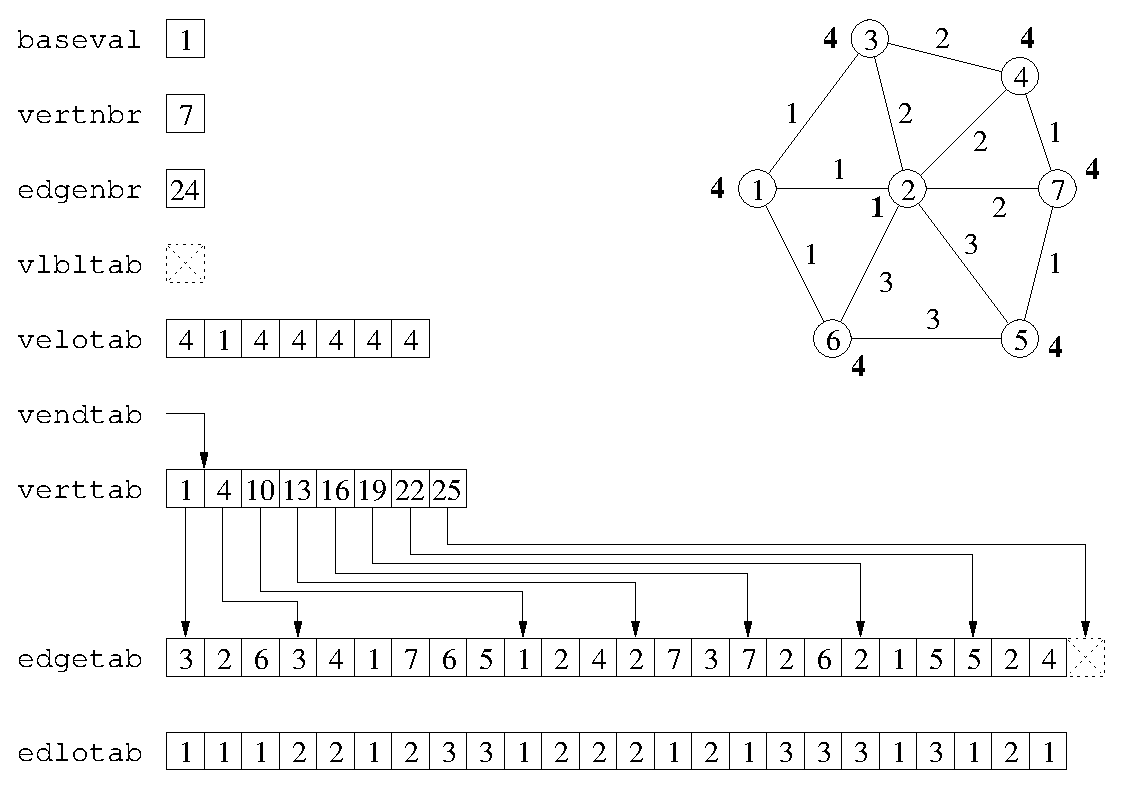
\includegraphics[scale=0.47]{s_f_gr1.eps}
\caption{Sample graph and its description by \libscotch\ arrays using
a compact edge array. Numbers within vertices are vertex indices, bold
numbers close to vertices are vertex loads, and numbers close to edges
are edge loads. Since the edge array is compact, $\mathtt{verttab}$ is
of size $\mathtt{vertnbr} + 1$ and $\mathtt{vendtab}$ points to
$\mathtt{verttab} + 1$.}
\label{fig-lib-graf-one}
\end{figure}

\begin{figure}
\centering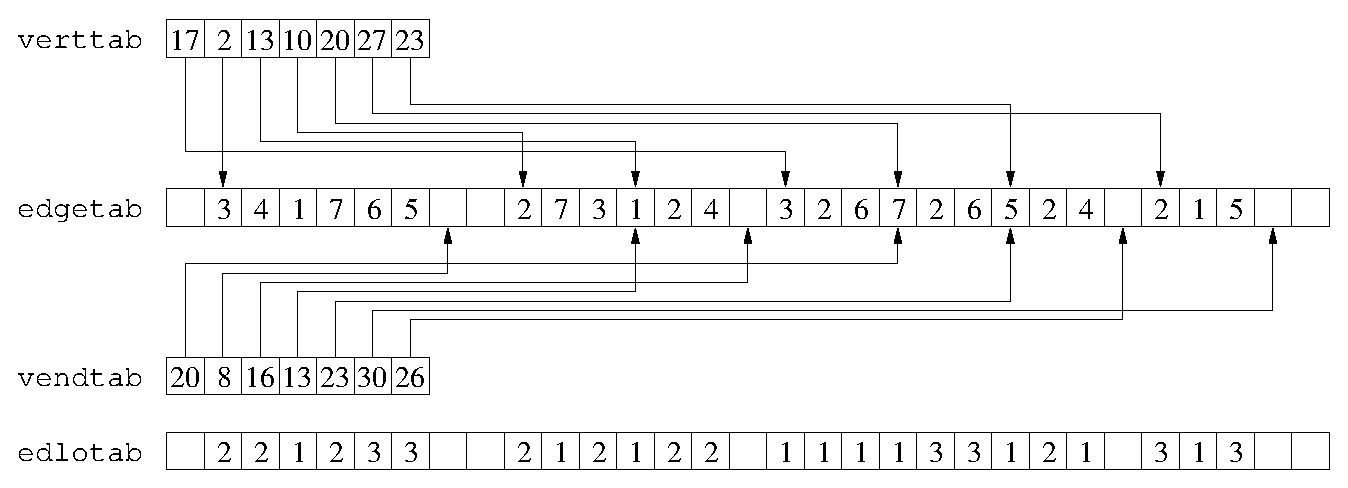
\includegraphics[scale=0.47]{s_f_gr2.eps}
\caption{Adjacency structure of the sample graph of
Figure~\protect\ref{fig-lib-graf-one} with disjoint edge and
edge load arrays. Both $\mathtt{verttab}$ and $\mathtt{vendtab}$ are of
size $\mathtt{vertnbr}$. This allows for the handling of dynamic
graphs, the structure of which can evolve with time.}
\label{fig-lib-graf-two}
\end{figure}

Dynamic graphs can be handled elegantly by using the
$\mathtt{vendtab}$ array. In order to dynamically manage graphs, one
just has to allocate $\mathtt{verttab}$, $\mathtt{vendtab}$ and
$\mathtt{edgetab}$ arrays that are large enough to contain all of the
expected new vertex and edge data. Original vertices are labeled
starting from $\mathtt{baseval}$, leaving free space at the end of the
arrays. To remove some vertex $i$, one just has to replace
$\mathtt{verttab[}i\mathtt{]}$ and
$\mathtt{vendtab[}i\mathtt{]}$ with the values of
$\mathtt{verttab[\lbt vertnbr}\lbt -1\mathtt{]}$ and
$\mathtt{vendtab[\lbt vertnbr}\lbt -1\mathtt{]}$, respectively, and
browse the adjacencies of all neighbors of former vertex
$\mathtt{vertnbr}-1$ such that all $(\mathtt{vertnbr}-1)$ indices are
turned into $i$s. Then, $\mathtt{vertnbr}$ must be decremented, and
\texttt{SCOTCH\_\lbt graphBuild()} must be called to account for the
change of topology. If a graph building routine such as
\texttt{SCOTCH\_\lbt graph\lbt Load()} or
\texttt{SCOTCH\_\lbt graph\lbt Build()} had 
already been called on the \texttt{SCOTCH\_\lbt Graph} structure,
\texttt{SCOTCH\_\lbt graph\lbt Free()} has to be called first in order
to free the internal structures associated with the older version of
the graph; else, these data would be lost, which would result in
memory leakage.

To add a new vertex, one has to fill $\mathtt{verttab[\lbt vertnbr}
-1\mathtt{]}$ and $\mathtt{vendtab[\lbt vertnbr}\lbt -1\mathtt{]}$
with the starting and end indices of the adjacency sub-array of the
new vertex. Then, the adjacencies of its neighbor vertices must also
be updated to account for it. If free space had been reserved at the
end of each of the neighbors, one just has to increment the
$\mathtt{vendtab[}i\mathtt{]}$ values of every neighbor $i$, and add
the index of the new vertex at the end of the adjacency sub-array. If
the sub-array cannot be extended, then it has to be copied elsewhere
in the edge array, and both $\mathtt{verttab[}i\mathtt{]}$ and
$\mathtt{vendtab[}i\mathtt{]}$ must be updated accordingly. With
simple housekeeping of free areas of the edge array, dynamic arrays
can be updated with as little data movement as possible.

\subsubsection{Mesh format}
\label{sec-lib-format-mesh}

Since meshes are basically bipartite graphs, source meshes are also
described by means of adjacency lists. The description of a mesh
requires several \texttt{SCOTCH\_Num} scalars and arrays, as shown in
Figure~\ref{fig-lib-mesh-one}. They have the following meaning:
\begin{itemize}
\iteme[{\tt velmbas}]
Base value for element indexings.
\iteme[{\tt vnodbas}]
Base value for node indexings. The base value of the underlying graph,
$\mathtt{baseval}$, is set as $\min(\mathtt{velmbas}, \mathtt{vnodbas})$.
\iteme[{\tt velmnbr}]
Number of element vertices in mesh.
\iteme[{\tt vnodnbr}]
Number of node vertices in mesh.
The overall number of vertices in the underlying graph,
$\mathtt{vertnbr}$, is set as $\mathtt{velmnbr} +\mathtt{vnodnbr}$.
\iteme[{\tt edgenbr}]
Number of arcs in mesh. Since edges are represented by both of their
ends, the number of edge data in the mesh is twice the number of
edges.
\iteme[{\tt verttab}]
Array of start indices in $\mathtt{edgetab}$ of vertex (that is, both
elements and nodes) adjacency sub-arrays.
\iteme[{\tt vendtab}]
Array of after-last indices in $\mathtt{edgetab}$ of vertex adjacency
sub-arrays. For any element or node vertex $i$, with
$\mathtt{baseval} \leq i <
(\mathtt{baseval} + \mathtt{vertnbr})$,
$\mathtt{vendtab[}i\mathtt{]} - \mathtt{verttab[}i\mathtt{]}$ is the
degree of vertex $i$, and the indices of the neighbors of $i$ are
stored in $\mathtt{edgetab}$ from
$\mathtt{edgetab[\lbt verttab[}i\mathtt{]]}$  to
$\mathtt{edgetab[\lbt vendtab[}i\mathtt{]} - 1\mathtt{]}$, inclusive.

When all vertex adjacency lists are stored in order in
$\mathtt{edgetab}$, it is possible to save memory by not allocating
the physical memory for $\mathtt{vendtab}$. In this case, illustrated
in Figure~\ref{fig-lib-mesh-one}, $\mathtt{verttab}$ is of size
$(\mathtt{vertnbr} + 1)$ and $\mathtt{vendtab}$ points to
$(\mathtt{verttab} + 1)$.
This case is referred to as the ``compact edge array'' case, such that
$\mathtt{verttab}$ is sorted in ascending order,
$\mathtt{verttab[\lbt baseval]} = \mathtt{baseval}$
and $\mathtt{verttab[\lbt baseval} + \mathtt{vertnbr]} = (\mathtt{baseval} + \mathtt{edgenbr})$.
\iteme[{\tt velotab}]
Array, of size $\mathtt{vertnbr}$, holding the integer load associated
with each vertex.
\end{itemize}

\begin{figure}
\centering\includegraphics[scale=0.47]{s_f_me1.eps}
\caption{Sample mesh and its description by \libscotch\ arrays using a
compact edge array. Numbers within vertices are vertex indices. Since the
edge array is compact, $\mathtt{verttab}$ is of size $(\mathtt{vertnbr} +
1)$ and $\mathtt{vendtab}$ points to $(\mathtt{verttab} + 1)$.}
\label{fig-lib-mesh-one}
\end{figure}

As for graphs, it is possible to handle elegantly dynamic meshes by
means of the $\mathtt{verttab}$ and $\mathtt{vendtab}$ arrays. There
is, however, an additional constraint, which is that mesh nodes and
elements must be ordered consecutively. The solution to fulfill this
constraint in the context of mesh ordering is to keep a set of empty
elements (that is, elements which have no node adjacency attached to
them) between the element and node arrays. For instance,
Figure~\ref{fig-lib-mesh-two} represents a $4$-element mesh with $6$
nodes, and such that $4$ element vertex slots have been reserved for
new elements and nodes. These slots are empty elements for which
$\mathtt{verttab[}i\mathtt{]}$ equals $\mathtt{vendtab[}i\mathtt{]}$,
irrespective of these values, since they will not lead to any memory
access in $\mathtt{edgetab}$.

\begin{figure}
\centering\includegraphics[scale=0.47]{s_f_me2.eps}
\caption{Sample mesh and its description by \libscotch\ arrays, with
nodes numbered first and elements numbered last. In order to allow for
dynamic re-meshing, empty elements (in grey) have been inserted between
existing node and element vertices.}
\label{fig-lib-mesh-two}
\end{figure}

Using this layout of vertices, new nodes and elements can be created
by growing the element and node sub-arrays into the empty element
sub-array, by both of its sides, without having to re-write the whole
mesh structure, as illustrated in
Figure~\ref{fig-lib-mesh-three}. Empty elements are transparent to the
mesh ordering routines, which base their work on node vertices only.
Users who want to update the arrays of a mesh that has already
been declared using the {\tt SCOTCH\_\lbt mesh\lbo Build()} routine must
call {\tt SCOTCH\_\lbt mesh\lbo Exit()} prior to updating the mesh arrays,
and then call {\tt SCOTCH\_\lbt mesh\lbo Build()} again after the arrays
have been updated, so that the {\tt SCOTCH\_\lbt Mesh} structure remains
consistent with the new mesh data.

\begin{figure}
\centering\includegraphics[scale=0.47]{s_f_me3.eps}
\caption{Re-meshing of the mesh of Figure~\protect\ref{fig-lib-mesh-two}.
New node vertices have been added at the end of the vertex sub-array,
new elements have been added at the beginning of the element sub-array,
and vertex base values have been updated accordingly. Node adjacency
lists that could not fit in place have been added at the end of the edge
array, and some of the freed space has been re-used for new adjacency
lists. Element adjacency lists do not require moving in this case, as
all of the elements have the name number of nodes.}
\label{fig-lib-mesh-three}
\end{figure}

\subsubsection{Geometry format}
\label{sec-lib-format-geom}

Geometry data is always associated with a graph or a mesh. It is
simply made of a single array of double-precision values which
represent the coordinates of the vertices of a graph, or of
the node vertices of a mesh, in vertex order. The fields of
a geometry structure are the following:
\begin{itemize}
\iteme[{\tt dimnnbr}]
Number of dimensions of the graph or of the mesh, which can be $1$,
$2$, or $3$.
\iteme[{\tt geomtab}]
Array of coordinates. This is an array of double precision values
organized as an array of $(x)$, or $(x,y)$, or $(x,y,z)$ tuples,
according to $\mathtt{dimnnbr}$. Coordinates that are not used
(e.g. the $z$ coordinates for a bidimentional object) are not
allocated. Therefore, the $x$ coordinate of some graph vertex $i$ is
located at $\mathtt{geomtab}\mbox{\tt [}(i - \mathtt{baseval}) *
\mathtt{dimnnbr}  + \mathtt{baseval}\mbox{\tt ]}$, its $y$ coordinate
is located at $\mathtt{geomtab}\mbox{\tt [}(i - \mathtt{baseval}) *
  \mathtt{dimnnbr} + \mathtt{baseval} + 1\mbox{\tt ]}$ if
$\mathtt{dimnnbr} \geq 2$, and its $z$ coordinate is located at
$\mathtt{geomtab}\mbox{\tt [}(i - \mathtt{baseval}) * \mathtt{dimnnbr}
+ \mathtt{baseval} + 2\mbox{\tt ]}$ if $\mathtt{dimnnbr} =
3$. Whenever the geometry is associated with a mesh,
only node vertices are considered, so the $x$ coordinate of some mesh
node vertex $i$, with $\mathtt{vnodbas} \leq i$, is located
at $\mathtt{geomtab}\mbox{\tt [}(i - \mathtt{vnodbas}) *
\mathtt{dimnnbr} + \mathtt{baseval}\mbox{\tt ]}$, its $y$ coordinate
is located at $\mathtt{geomtab}\mbox{\tt [}(i - \mathtt{vnodbas}) *
\mathtt{dimnnbr} + \mathtt{baseval} + 1\mbox{\tt ]}$ if
$\mathtt{dimnnbr} \geq 2$, and its $z$ coordinate is located at
$\mathtt{geomtab}\mbox{\tt [}(i - \mathtt{vnodbas}) * \mathtt{dimnnbr}
+ \mathtt{baseval} + 2\mbox{\tt ]}$ if $\mbox{\tt dimnnbr} = 3$.
\end{itemize}

\subsubsection{Block ordering format}
\label{sec-lib-format-order}

Block orderings associated with graphs and meshes are described by
means of block and permutation arrays, made of {\tt SCOTCH\_Num}s, as
shown in Figure~\ref{fig-lib-ord-block}. In order for all orderings to
have the same structure, irrespective of whether they are created from
graphs or meshes, all ordering data indices start from {\tt baseval},
even when they refer to a mesh the node vertices of which are labeled
from a $\mathtt{vnodbas}$ index such that $\mathtt{vnodbas} >
\mathtt{baseval}$. Consequently, row indices are related to vertex
indices in memory in the following way: row $i$ is associated with
vertex $i$ of the {\tt SCOTCH\_\lbt Graph} structure if the ordering
was computed from a graph, and with node vertex $i + (\mbox{\tt
vnodbas} - \mathtt{baseval})$ of the {\tt SCOTCH\_\lbt Mesh}
structure if the ordering was computed from a mesh.
Block orderings are made of the following data:
\begin{itemize}
\iteme[{\tt permtab}]
Array holding the permutation of the reordered matrix. Thus, if $k =
\mathtt{permtab}\mbox{\tt [}\mathit{i}\mbox{\tt ]}$, then row $i$ of
the original matrix is now row $k$ of the reordered matrix, that is,
row $i$ is the $k^{\mathrm{th}}$ pivot.
\iteme[{\tt peritab}]
Inverse permutation of the reordered matrix. Thus, if
$i = \mathtt{peritab}\mbox{\tt [}\mathit{k}\mbox{\tt ]}$, then row $k$
of the reordered matrix was row $i$ of the original matrix.
\iteme[{\tt cblknbr}]
Number of column blocks (that is, supervariables) in the block ordering.
\iteme[{\tt rangtab}]
Array of ranges for the column blocks. Column block $c$, with
$\mathtt{baseval} \leq c < (\mathtt{cblknbr} + \mathtt{baseval})$,
contains columns with indices ranging from
$\mathtt{rangtab}\mbox{\tt [}\mathit{i}\mbox{\tt ]}$ to
$\mathtt{rangtab}\mbox{\tt [}\mathit{i} + 1\mbox{\tt ]}$, exclusive,
in the reordered matrix. Indices in $\mathtt{rangtab}$ are
based. Therefore,
$\mathtt{rangtab}\mbox{\tt [}\mathtt{baseval}\mbox{\tt ]}$ is always
equal to $\mathtt{baseval}$, and
$\mathtt{rangtab}\mbox{\tt [}\mathtt{cblknbr} +
\mathtt{baseval}\mbox{\tt ]}$ is always equal to
$\mathtt{vertnbr} + \mathtt{baseval}$ for graphs and
to $\mathtt{vnodnbr} + \mathtt{baseval}$ for meshes.
In order to avoid memory errors when column blocks are all single
columns, the size of {\tt rangtab} must always be one more than the
number of columns, that is, $\mathtt{vertnbr} + 1$ for graphs and
$\mathtt{vnodnbr} + 1$ for meshes.
\iteme[{\tt treetab}]
Array of ascendants of permuted column blocks in the separators tree.
{\tt treetab[i]} is the index of the father of column block $i$ in the
separators tree, or $-1$ if column block $i$ is the root of the
separators tree. Whenever separators or leaves of the separators tree
are split into sub-blocks, as the block splitting, minimum fill or minimum
degree methods do, all sub-blocks of the same level are linked to the
column block of higher index belonging to the closest separator
ancestor. Indices in {\tt treetab} are based, in the same way as for
the other blocking structures. See Figure~\ref{fig-lib-ord-block} for
a complete example.
\end{itemize}

\begin{figure}
\centering\includegraphics[scale=0.47]{s_f_orb.eps}
\caption{Arrays resulting from the ordering by complete nested
dissection of a 4 by 3 grid based from $1$. Leftmost grid is the
original grid, and righmost grid is the reordered grid, with
separators shown and column block indices written in bold.}
% using strategy  n{sep=hf{bal=0},ole=s,ose=s}
\label{fig-lib-ord-block}
\end{figure}

\subsection{Strategy strings}

The behavior of the mapping and block ordering routines of the
\libscotch\ library is parametrized by means of strategy strings,
which describe how and when given partitioning or ordering methods
should be applied to graphs and subgraphs, or to meshes and submeshes.

\subsubsection{Using default strategy strings}
\label{sec-lib-format-strat-default}

While strategy strings can be built by hand, according to the syntax
given in the next sections, users who do not have specific needs can
take advantage of default strategies already implemented in the
\libscotch, which will yield very good results in most cases. By
doing so, they will spare themselves the hassle of updating their
strategies to comply to subsequent syntactic changes, and they will
benefit from the availability of new partitioning or ordering methods
as soon as they are released.

The simplest way to use default strategy strings is to avoid
specifying any. By initializing a strategy object, by means of the
{\tt SCOTCH\_\lbt stratInit} routine, and by using the initialized
strategy object as is, without further parametrization, this object
will be filled with a default strategy when passing it as a parameter
to the next partitioning or ordering routine to be called. On return,
the strategy object will contain a fully specified strategy, tailored
for the type of operation which has been requested. Consequently, a
fresh strategy object that was used to partition a graph cannot be
used afterward as a default strategy when calling an ordering routine,
for instance, as partitioning and ordering strategies are incompatible.

The \libscotch\ also provides helper routines which allow users to
express their preferences on the kind of strategy that they
need. These helper routines, which are of the form
{\tt SCOTCH\_\lbt strat\lbt *\lbt Build} (see
Section~\ref{sec-lib-func-stratgraphclusterbuild} and after), tune
default strategy strings according to parameters provided by the user,
such as the requested number of parts (used as a hint to select the
most efficient partitioning routines), the desired maximum load
imbalance ratio, and a set of preference flags. While some of these
flags are antagonistic, most of them can be combined, by means of
addition or ``binary or'' operators. These flags are the following.
They are grouped by application class.

\paragraph{Global flags}

\begin{itemize}
\iteme[{\tt SCOTCH\_STRATDEFAULT}]
Default behavior. No flags are set.
\iteme[{\tt SCOTCH\_STRATBALANCE}]
Enforce load balance as much as possible.
\iteme[{\tt SCOTCH\_STRATQUALITY}]
Privilege quality over speed.
\iteme[{\tt SCOTCH\_STRATSAFETY}]
Do not use methods that can lead to the occurrence of problematic
events, such as floating point exceptions, which could not be properly
handled by the calling software.
\iteme[{\tt SCOTCH\_STRATSPEED}]
Privilege speed over quality.
\end{itemize}

\paragraph{Mapping and partitioning flags}

\begin{itemize}
\iteme[{\tt SCOTCH\_STRATRECURSIVE}]
Use only recursive bipartitioning methods, and not direct k-way
methods. When this flag is not set, any combination of methods can be
used, so as to achieve the best result according to other user
preferences.
\iteme[{\tt SCOTCH\_STRATREMAP}]
Use the strategy for remapping an existing partition.
\end{itemize}

\paragraph{Ordering flags}

\begin{itemize}
\iteme[{\tt SCOTCH\_STRATDISCONNECTED}]
Find and handle independently disconnected components.
\iteme[{\tt SCOTCH\_STRATLEVELMAX}]
Create at most the prescribed levels of nested dissection separators.
\iteme[{\tt SCOTCH\_STRATLEVELMIN}]
Create at least the prescribed levels of nested dissection separators.
When used in conjunction with {\tt SCOTCH\_\lbt STRAT\lbt LEVEL\lbt
MAX}, the exact number of nested dissection levels will be performed,
unless the graph to order is too small.
\iteme[{\tt SCOTCH\_STRATLEAFSIMPLE}]
Order nested dissection leaves as cheaply as possible.
\iteme[{\tt SCOTCH\_STRATSEPASIMPLE}]
Order nested dissection separators as cheaply as possible.
\end{itemize}

\subsubsection{Mapping strategy strings}
\label{sec-lib-format-map}

At the time being, mapping methods only apply to graphs, as there is
not yet a mesh mapping tool in the \scotch\ package.

Mapping strategies are made of methods, with optional parameters enclosed
between curly braces, and separated by commas, in the form of
{\it method\/}{[{\tt \{}{\it parameters\/}{\tt \}}]}\enspace.
The currently available mapping methods are the following.

\begin{itemize}
\iteme[{\tt b}]
Band method. This method builds a band graph of given width around the
current frontier of the k-way partition to which it is applied, and
calls a graph mapping strategy to refine the equivalent k-way
partition of the band graph. Then, the refined frontier of the band
graph is projected back to the current graph. This method was
initially presented in~\cite{chpe06a} in the case of bipartitioning.
The parameters of the band bipartitioning method are listed below.
\begin{itemize}
\iteme[{\tt bnd=}{\it strat}]
Set the graph mapping strategy to be used on the band graph.
\iteme[{\tt org=}{\it strat}]
Set the fallback graph mapping strategy to be used on the
original graph if the band graph strategy could not be used. The three
cases which require the use of this fallback strategy are the
following. First, if the separator of the original graph is empty,
which makes it impossible to compute a band graph. Second, if any part
of the band graph to be built is of the same size as the one of the
original graph. Third, if the application of the {\tt bnd}
bipartitioning method to the band graph leads to a situation where any
two anchor vertices are placed in the same part.
\iteme[{\tt width=}{\it val}]
Set the width of the band graph. All graph vertices that are at a
distance less than or equal to {\it val} from any frontier vertex
are kept in the band graph.
\end{itemize}
\iteme[{\tt d}]
Diffusion method. This method, presented in~\cite{pell07b} in the case
of bipartitioning, flows $k$ kinds of antagonistic liquids from $k$
source vertices, and sets the new frontier as the limit between vertices
which contain different kinds of liquids. Because
selecting the source vertices is essential to the obtainment of useful
results, this method has been hard-coded so that the $k$ source
vertices are the $k$ vertices of highest indices, since in the band
method these are the anchor vertices which represent all of the removed
vertices of each part. Therefore, this method must be used on band
graphs only, or on specifically crafted graphs. Applying it to any
other graphs is very likely to lead to extremely poor results.
The physical analogy of this method loses weight when it is applied to
target architectures that are not complete graphs.
The parameters of the diffusion mapping method are listed below.
\begin{itemize}
\iteme[{\tt dif=}{\it rat}]
Fraction of liquid which is diffused to neighbor vertices at each
pass. To achieve convergence, the sum of the {\tt dif} and {\tt rem}
parameters must be equal to $1$, but in order to speed-up the diffusion
process, other combinations of higher sum can be tried. In this case,
the number of passes must be kept low, to avoid numerical overflows
which would make the results useless.
\iteme[{\tt pass=}{\it nbr}]
Set the number of diffusion sweeps performed by the algorithm. This
number depends on the width of the band graph to which the diffusion
method is applied. Useful values range from $30$ to $500$ according
to chosen {\tt dif} and {\tt rem} coefficients.
\iteme[{\tt rem=}{\it rat}]
Fraction of liquid which remains on vertices at each pass. See above.
\end{itemize}
\iteme[{\tt f}]
$k$-way Fiduccia-Mattheyses method. The parameters of the
Fiduccia-Mattheyses method are listed below.
\begin{itemize}
\iteme[{\tt bal=}{\it rat}]
Set the maximum weight imbalance ratio to the given fraction of
the subgraph vertex weight. Common values are around $0.01$, that
is, one percent.
\iteme[{\tt move=}{\it nbr}]
Maximum number of hill-climbing moves that can be performed before a
pass ends. During each of its passes, the Fiduccia-Mattheyses
algorithm repeatedly swaps vertices between parts so as to
minimize the cost function. A pass completes either when all of the
vertices have been moved once, or if too many swaps that do not
decrease the value of the cost function have been performed. Setting
this value to zero turns the Fiduccia-Mattheyses algorithm into a
gradient-like method, which may be used to quickly refine partitions
during the uncoarsening phase of the multilevel method.
\iteme[{\tt pass=}{\it nbr}]
Set the maximum number of optimization passes performed by the
algorithm. The Fiduccia-Mattheyses algorithm stops as soon as a pass
has not yielded any improvement of the cost function, or when the
maximum number of passes has been reached. Value $-1$ stands for an
infinite number of passes, that is, as many as needed by the algorithm
to converge.
\end{itemize}
\iteme[{\tt m}]
Multilevel method. The parameters of the multilevel method are listed below.
\begin{itemize}
\iteme[{\tt asc=}{\it strat}]
Set the strategy that is used to refine the mappings obtained
at ascending levels of the uncoarsening phase by projection of the
mappings computed for coarser graphs.
This strategy is not applied to the coarsest graph, for which only the
{\tt low} strategy is used.
\iteme[{\tt low=}{\it strat}]
Set the strategy that is used to compute the mapping of the
coarsest graph, at the lowest level of the coarsening process.
\iteme[{\tt rat=}{\it rat}]
Set the threshold maximum coarsening ratio over which graphs are no longer
coarsened. The ratio of any given coarsening cannot be less that $0.5$
(case of a perfect matching), and cannot be greater than $1.0$.
Coarsening stops when either the coarsening ratio is above the maximum
coarsening ratio, or the graph has fewer vertices than the minimum number of
vertices allowed.
\iteme[{\tt vert=}{\it nbr}]
Set the threshold under which graphs are no longer
coarsened. Coarsening stops when either the coarsening ratio is above
the maximum coarsening ratio, or the graph would have fewer vertices
than the minimum number of vertices allowed. When the target
architecture is a variable-sized architecture, coarsening stops when
the coarsened graph would have less than \mbox{\it nbr} vertices. When
the target architecture is a regular, fixed-size, architecture,
coarsening stops when each subdomain would have less than \mbox{\it
  nbr} vertices, that is, when the size of the coarsened graph would
have less than $\mbox{\it nbr}\times\mathtt{domnnbr}$ vertices,
where $\mathtt{domnnbr}$ is the number of vertices in the target
architecture.
\end{itemize}
\iteme[{\tt r}]
Dual Recursive Bipartitioning mapping algorithm, as defined in
section~\ref{sec-algo-drb}. The parameters of the DRB mapping method are
listed below.
\begin{itemize}
\iteme[{\tt job=}{\it tie}]
The {\it tie\/} flag defines how new jobs are stored in job pools.
\begin{itemize}
\iteme[{\tt t}]
Tie job pools together. Subjobs are stored in same pool as their parent job.
This is the default behavior, as it proves the most efficient in practice.
\iteme[{\tt u}]
Untie job pools. Subjobs are stored in the next job pool to be processed.
\end{itemize}
\iteme[{\tt map=}{\it tie}]
The {\it tie\/} flag defines how results of bipartitioning jobs are
propagated to jobs still in pools.
\begin{itemize}
\iteme[{\tt t}]
Tie both mapping tables together. Results are immediately available to jobs
in the same job pool. This is the default behavior.
\iteme[{\tt u}]
Untie mapping tables. Results are only available to jobs of next pool to be
processed.
\end{itemize}
\iteme[{\tt poli=}{\it policy}]
Select jobs according to policy {\it policy}. Job selection policies
define how bipartitioning jobs are ordered within the currently active job
pool. Valid policy flags are
\begin{itemize}
\iteme[{\tt L}]
Most neighbors of higher level.
\iteme[{\tt l}]
Highest level.
\iteme[{\tt r}]
Random.
\iteme[{\tt S}]
Most neighbors of smaller size. This is the default behavior.
\iteme[{\tt s}]
Biggest size.
\end{itemize}
\iteme[{\tt sep=}{\it strat}]
Apply bipartitioning strategy {\it strat\/} to each bipartitioning job.
A bipartitioning strategy is made of one or several bipartitioning methods,
which can be combined by means of strategy operators. Graph
bipartitioning strategies are described below.
\end{itemize}
\iteme[{\tt x}]
Exactifier method, as defined in Section~\ref{sec-algo-map-exact}.
This greedy algorithm refines the current mapping so as to reduce load
imbalance as much as possible. Since this method does not consider
communication minimization, its use should be restricted to cases
where achieving load balance is critical and where recursive
bipartitioning may fail to achieve it, because of very irregular
vertex loads.
\end{itemize}

\subsubsection{Graph bipartitioning strategy strings}
\label{sec-lib-format-bipart}

A graph bipartitioning strategy is made of one or several graph
bipartitioning methods, which can be combined by means of strategy
operators. Strategy operators are listed below, by increasing
precedence.

\begin{itemize}
\iteme[{\it strat1\/}{\tt |}{\it strat2}]
Selection operator. The result of the selection is the best bipartition of
the two that are obtained by the separate application of {\it strat1\/} and
{\it strat2\/} to the current bipartition.
\iteme[{\it strat1$\:$}{\it strat2}]
Combination operator. Strategy {\it strat2\/} is applied to the bipartition
resulting from the application of strategy {\it strat1\/} to the current
bipartition. Typically, the first method used should compute an initial
bipartition from scratch, and every following method should use the
result of the previous one at its starting point.
\iteme[{\tt (}{\it strat\/}{\tt )}]
Grouping operator.
The strategy enclosed within the parentheses is treated as a single
bipartitioning method.
\iteme[{\tt /}{\it cond\/}{\tt ?}{\it strat1\/}{[{\tt :}{\it strat2}]{\tt ;}}]
Condition operator. According to the result of the evaluation of condition
{\it cond}, either {\it strat1\/} or {\it strat2\/} (if it is present) is
applied. The condition applies to the characteristics of the current active
graph, and can be built from logical and relational operators. Conditional
operators are listed below, by increasing precedence.
\begin{itemize}
\iteme[{\it cond1\/}{\tt |}{\it cond2}]
Logical or operator. The result of the condition is true if {\it cond1\/}
or {\it cond2\/} are true, or both.
\iteme[{\it cond1\/}{\tt \&}{\it cond2}]
Logical and operator. The result of the condition is true only if both
{\it cond1\/} and {\it cond2\/} are true.
\iteme[{\tt !}{\it cond}]
Logical not operator. The result of the condition is true only if
{\it cond\/} is false.
\iteme[{\it var} {\it relop} {\it val}]
Relational operator, where {\it var\/} is a graph variable, {\it val\/} is
either a graph variable or a constant of the type of variable {\it var\/}, and
{\it relop\/} is one of '{\tt\verb+<+}', '{\tt\verb+=+}', and '{\tt\verb+>+}'.
The graph variables are listed below, along with their types.
\begin{itemize}
\iteme[{\tt deg}]
The average degree of the current graph.
Float.
\iteme[{\tt edge}]
The number of arcs (which is twice the number of edges) of the current graph.
Integer.
\iteme[{\tt load}]
The overall vertex load (weight) of the current graph.
Integer.
\iteme[{\tt load0}]
The vertex load of the first subset of the current bipartition of the current
graph.
Integer.
\iteme[{\tt vert}]
The number of vertices of the current graph.
Integer.
\end{itemize}
\end{itemize}
\iteme[{\it method\/}{[{\tt \{}{\it parameters\/}{\tt \}}]}]
Bipartitioning method. For bipartitioning methods that can be
parametrized, parameter settings may be provided after the method
name. Parameters must be separated by commas, and the whole list
be enclosed between curly braces.
\end{itemize}
The currently available graph bipartitioning methods are the following.
\begin{itemize}
\iteme[{\tt b}]
Band method. This method builds a band graph of given width around the
current frontier of the graph to which it is applied, and
calls a graph bipartitioning strategy to refine the equivalent
bipartition of the band graph. Then, the refined frontier of the band
graph is projected back to the current graph. This method, presented
in~\cite{chpe06a}, was created to reduce the cost of vertex separator
refinement algorithms in a multilevel context, but it improves
partition quality too. The same behavior is observed for graph
bipartitioning. The parameters of the band bipartitioning method are
listed below.
\begin{itemize}
\iteme[{\tt bnd=}{\it strat}]
Set the graph bipartitioning strategy to be used on the band graph.
\iteme[{\tt org=}{\it strat}]
Set the fallback graph bipartitioning strategy to be used on the
original graph if the band graph strategy could not be used. The three
cases which require the use of this fallback strategy are the
following. First, if the separator of the original graph is empty,
which makes it impossible to compute a band graph. Second, if any part
of the band graph to be built is of the same size as the one of the
original graph. Third, if the application of the {\tt bnd}
bipartitioning method to the band graph leads to a situation where both
anchor vertices are placed in the same part.
\iteme[{\tt width=}{\it val}]
Set the width of the band graph. All graph vertices that are at a
distance less than or equal to {\it val} from any frontier vertex
are kept in the band graph.
\end{itemize}
\iteme[{\tt d}]
Diffusion method. This method, presented in~\cite{pell07b}, flows two
kinds of antagonistic liquids, scotch and anti-scotch, from two source
vertices, and sets the new frontier as the limit between vertices
which contain scotch and the ones which contain anti-scotch. Because
selecting the source vertices is essential to the obtainment of useful
results, this method has been hard-coded so that the two source
vertices are the two vertices of highest indices, since in the band
method these are the anchor vertices which represent all of the removed
vertices of each part. Therefore, this method must be used on band
graphs only, or on specifically crafted graphs. Applying it to any
other graphs is very likely to lead to extremely poor results.
The parameters of the diffusion bipartitioning method are
listed below.
\begin{itemize}
\iteme[{\tt dif=}{\it rat}]
Fraction of liquid which is diffused to neighbor vertices at each
pass. To achieve convergence, the sum of the {\tt dif} and {\tt rem}
parameters must be equal to $1$, but in order to speed-up the diffusion
process, other combinations of higher sum can be tried. In this case,
the number of passes must be kept low, to avoid numerical overflows
which would make the results useless.
\iteme[{\tt pass=}{\it nbr}]
Set the number of diffusion sweeps performed by the algorithm. This
number depends on the width of the band graph to which the diffusion
method is applied. Useful values range from $30$ to $500$ according
to chosen {\tt dif} and {\tt rem} coefficients.
\iteme[{\tt rem=}{\it rat}]
Fraction of liquid which remains on vertices at each pass. See above.
\end{itemize}
\iteme[{\tt f}]
Fiduccia-Mattheyses method. The parameters of the Fiduccia-Mattheyses method
are listed below.
\begin{itemize}
\iteme[{\tt bal=}{\it rat}]
Set the maximum weight imbalance ratio to the given fraction of
the subgraph vertex weight. Common values are around $0.01$, that
is, one percent.
\iteme[{\tt move=}{\it nbr}]
Maximum number of hill-climbing moves that can be performed before a
pass ends. During each of its passes, the Fiduccia-Mattheyses
algorithm repeatedly swaps vertices between the two parts so as to
minimize the cost function. A pass completes either when all of the
vertices have been moved once, or if too many swaps that do not
decrease the value of the cost function have been performed. Setting
this value to zero turns the Fiduccia-Mattheyses algorithm into a
gradient-like method, which may be used to quickly refine partitions
during the uncoarsening phase of the multilevel method.
\iteme[{\tt pass=}{\it nbr}]
Set the maximum number of optimization passes performed by the
algorithm. The Fiduccia-Mattheyses algorithm stops as soon as a pass
has not yielded any improvement of the cost function, or when the
maximum number of passes has been reached. Value $-1$ stands for an
infinite number of passes, that is, as many as needed by the algorithm
to converge.
\end{itemize}
\iteme[{\tt g}]
Gibbs-Poole-Stockmeyer method. This method has only one parameter.
\begin{itemize}
\iteme[{\tt pass=}{\it nbr}]
Set the number of sweeps performed by the algorithm.
\end{itemize}
\iteme[{\tt h}]
Greedy-graph-growing method. This method has only one parameter.
\begin{itemize}
\iteme[{\tt pass=}{\it nbr}]
Set the number of runs performed by the algorithm.
\end{itemize}
\iteme[{\tt m}]
Multilevel method. The parameters of the multilevel method are listed below.
\begin{itemize}
\iteme[{\tt asc=}{\it strat}]
Set the strategy that is used to refine the partitions obtained
at ascending levels of the uncoarsening phase by projection of the
bipartitions computed for coarser graphs.
This strategy is not applied to the coarsest graph, for which only the
{\tt low} strategy is used.
\iteme[{\tt low=}{\it strat}]
Set the strategy that is used to compute the partition of the
coarsest graph, at the lowest level of the coarsening process.
\iteme[{\tt rat=}{\it rat}]
Set the threshold maximum coarsening ratio over which graphs are no longer
coarsened. The ratio of any given coarsening cannot be less that $0.5$
(case of a perfect matching), and cannot be greater than $1.0$.
Coarsening stops when either the coarsening ratio is above the maximum
coarsening ratio, or the graph has fewer vertices than the minimum number of
vertices allowed.
\iteme[{\tt vert=}{\it nbr}]
Set the threshold minimum graph size under which graphs are no longer
coarsened. Coarsening stops when either the coarsening ratio is above the
maximum coarsening ratio, or the coarsened graph would have fewer
vertices than the minimum number of vertices allowed.
\end{itemize}
\iteme[{\tt x}]
Exactifying method.
\iteme[{\tt z}]
Zero method. This method moves all of the vertices to the first
part. Its main use is to stop the bipartitioning process, if some
condition is true, when mapping onto variable-sized architectures (see
section~\ref{sec-algo-variable}).
\end{itemize}

\subsubsection{Vertex partitioning (with overlap) strategy strings}
\label{sec-lib-format-part-ovl}

Vertex partitioning is a special form of graph partitioning, in which
graphs are partitioned into a prescribed number of parts by means of
vertex separators rather than of edge separators like in
Section~\ref{sec-lib-format-map}. The load balance criterion also
differs from common practice: the load to be balanced across all parts
comprises not only the load of the vertices which belong to the part,
but also the load of all the separator vertices which are their
immediate neighbors. Consequently, the load of every separator vertex
is accounted for several times, in each of the parts it separates.

Vertex partitioning strategies are made of methods, with optional
parameters enclosed between curly braces, and separated by commas, in
the form of {\it method\/}{[{\tt \{}{\it parameters\/}{\tt \}}]}\enspace.
The currently available mapping methods are the following.

\begin{itemize}
\iteme[{\tt e}]
K-way edge partitioning method. The parameters of the Fiduccia-Mattheyses method
are listed below.
\begin{itemize}
\iteme[{\tt strat=}{\it strat}]
K-way partitioning strategy to be performed. It is in fact a k-way
mapping strategy, that is applied to a complete target graph of as
many vertices as the prescribed number of parts. The syntax of mapping
strategy strings is defined within section~\ref{sec-lib-format-map},
at page~\pageref{sec-lib-format-map}.
\end{itemize}
\iteme[{\tt f}]
Fiduccia-Mattheyses method. The parameters of the Fiduccia-Mattheyses method
are listed below.
\begin{itemize}
\iteme[{\tt bal=}{\it rat}]
Set the maximum weight imbalance ratio to the given fraction of
the subgraph vertex weight. Common values are around $0.01$, that
is, one percent.
\iteme[{\tt move=}{\it nbr}]
Maximum number of hill-climbing moves that can be performed before a
pass ends. During each of its passes, the Fiduccia-Mattheyses
algorithm repeatedly moves vertices between parts so as to
minimize the cost function. A pass completes either when all of the
vertices have been moved once, or if too many swaps that do not
decrease the value of the cost function have been performed. Setting
this value to zero turns the Fiduccia-Mattheyses algorithm into a
gradient-like method, which may be used to quickly refine partitions
during the uncoarsening phase of the multilevel method.
\iteme[{\tt pass=}{\it nbr}]
Set the maximum number of optimization passes performed by the
algorithm. The Fiduccia-Mattheyses algorithm stops as soon as a pass
has not yielded any improvement of the cost function, or when the
maximum number of passes has been reached. Value $-1$ stands for an
infinite number of passes, that is, as many as needed by the algorithm
to converge.
\end{itemize}
\iteme[{\tt h}]
Greedy-graph-growing method. This is a $k$-way version of the
original algorithm, in which parts are grown one after the
other. Consequently, depending on graph topology, this method is
likely to yield disconnected parts, with higher probability as the
number of part increases. This method has only one parameter.
\begin{itemize}
\iteme[{\tt pass=}{\it nbr}]
Set the number of runs performed by the algorithm.
\end{itemize}
\iteme[{\tt m}]
Multilevel method. The parameters of the multilevel method are listed below.
\begin{itemize}
\iteme[{\tt asc=}{\it strat}]
Set the strategy that is used to refine the partitions obtained
at ascending levels of the uncoarsening phase by projection of the
bipartitions computed for coarser graphs.
This strategy is not applied to the coarsest graph, for which only the
{\tt low} strategy is used.
\iteme[{\tt low=}{\it strat}]
Set the strategy that is used to compute the partition of the
coarsest graph, at the lowest level of the coarsening process.
\iteme[{\tt rat=}{\it rat}]
Set the threshold maximum coarsening ratio over which graphs are no longer
coarsened. The ratio of any given coarsening cannot be less that $0.5$
(case of a perfect matching), and cannot be greater than $1.0$.
Coarsening stops when either the coarsening ratio is above the maximum
coarsening ratio, or the graph has fewer vertices than the minimum number of
vertices allowed.
\iteme[{\tt vert=}{\it nbr}]
Set the threshold minimum number of vertices per part under which
graphs are no longer coarsened. Coarsening stops when either the
coarsening ratio is above the maximum coarsening ratio, or the graph
has fewer vertices than the minimum number of vertices allowed.
\end{itemize}
\iteme[{\tt r}]
Recursive bipartitioning algorithm. The parameters of the recursive
bipartitioning method are listed below.
\begin{itemize}
\iteme[{\tt sep=}{\it strat}]
Apply vertex (node) separation strategy {\it strat\/} to each
bipartitioning job. A node separation strategy is made of one or
several node separation methods, which can be combined by means of
strategy operators. Node separation strategies are described in
Section~\ref{sec-lib-format-nsep}.
\end{itemize}
\end{itemize}

\subsubsection{Ordering strategy strings}
\label{sec-lib-format-ord}

Ordering strategies are available both for graphs and for meshes.
An ordering strategy is made of one or several ordering methods, which
can be combined by means of strategy operators. The strategy
operators that can be used in ordering strategies are listed below, by
increasing precedence.

\begin{itemize}
\iteme[{\tt (}{\it strat\/}{\tt )}]
Grouping operator.
The strategy enclosed within the parentheses is treated as a single
ordering method.
\iteme[{\tt /}{\it cond\/}{\tt ?}{\it strat1\/}{[{\tt :}{\it strat2}]{\tt ;}}]
Condition operator. According to the result of the evaluation of
condition {\it cond}, either {\it strat1\/} or {\it strat2\/} (if it
is present) is applied. The condition applies to the characteristics
of the current node of the separators tree, and can be built from
logical and relational operators. Conditional operators are listed
below, by increasing precedence.
\begin{itemize}
\iteme[{\it cond1\/}{\tt |}{\it cond2}]
Logical or operator. The result of the condition is true if {\it cond1\/}
or {\it cond2\/} are true, or both.
\iteme[{\it cond1\/}{\tt \&}{\it cond2}]
Logical and operator. The result of the condition is true only if both
{\it cond1\/} and {\it cond2\/} are true.
\iteme[{\tt !}{\it cond}]
Logical not operator. The result of the condition is true only if
{\it cond\/} is false.
\iteme[{\it var} {\it relop} {\it val}]
Relational operator, where {\it var\/} is a node variable, {\it val\/} is
either a node variable or a constant of the type of variable {\it var}, and
{\it relop\/} is one of '{\tt\verb+<+}', '{\tt\verb+=+}', and '{\tt\verb+>+}'.
The node variables are listed below, along with their types.
\begin{itemize}
\iteme[{\tt edge}]
The number of vertices of the current subgraph.
Integer.
\iteme[{\tt levl}]
The level of the subgraph in the separators tree, starting from zero
for the initial graph at the root of the tree.
Integer.
\iteme[{\tt load}]
The overall vertex load (weight) of the current subgraph.
Integer.
\iteme[{\tt mdeg}]
The maximum degree of the current subgraph.
Integer.
\iteme[{\tt vert}]
The number of vertices of the current subgraph.
Integer.
\end{itemize}
\end{itemize}
\iteme[{\it method\/}{[{\tt \{}{\it parameters\/}{\tt \}}]}]
Graph or mesh ordering method. Available ordering methods are listed
below.
\end{itemize}
The currently available ordering methods are the following.
\begin{itemize}
\iteme[{\tt b}]
Blocking method. This method does not perform ordering by itself, but
is used as post-processing to cut into blocks of smaller sizes the
separators or large blocks produced by other ordering methods. This is
not useful in the context of direct solving methods, because the
off-diagonal blocks created by the splitting of large diagonal blocks
are likely to be filled at factoring time. However, in the context of
incomplete solving methods such as ILU(k)~\cite{heperaro04a}, it can
lead to a significant reduction of the required memory space and time,
because it helps carving large triangular blocks.
The parameters of the blocking method are described below.
\begin{itemize}
\iteme[{\tt cmin=}{\it wght}]
Set the minimum span of the resulting sub-blocks, in terms of column
weights. When the graph has no vertex weights (that is, all columns
have weight $1$), \texttt{cmin} represents the minimum number of
colums to be included within each sub-block.
For unweighted graphs, blocks larger than twice this minimum weight
are cut into sub-blocks of equal sizes (within one), having a number
of columns comprised between {\it wght} and $2${\it wght}. For
weighted graphs, the algorithm performs in a best effort to achieve
this goal.
\\
The definition of {\it size} depends on the size of the graph
to order. Large graphs cannot afford very small values, because the
number of blocks becomes much too large and limits the acceleration
of BLAS~3 routines, while large values do not help reducing enough
the complexity of ILU(k) solving.
\iteme[{\tt strat=}{\it strat}]
Ordering strategy to be performed. After the ordering strategy is
applied, the resulting separators tree is traversed and all of the
column blocks that are larger than $2${\it size} are split into
smaller column blocks, without changing the ordering that has been
computed.
\end{itemize}
\iteme[{\tt c}]
\label{sec-lib-meth-compress}
Compression method~\cite{ashc95}.
The parameters of the compression method are listed below.
\begin{itemize}
\iteme[{\tt rat=}{\it rat}]
Set the compression ratio over which graphs and meshes will not be
compressed. Useful values range between $0.7$ and $0.8$.
\iteme[{\tt cpr=}{\it strat}]
Ordering strategy to use on the compressed graph or mesh if its size
is below the compression ratio times the size of the original graph
or mesh.
\iteme[{\tt unc=}{\it strat}]
Ordering strategy to use on the original graph or mesh if the size of
the compressed graph or mesh were above the compression ratio times
the size of the original graph or mesh.
\end{itemize}
\iteme[{\tt d}]
Block Halo Approximate Minimum Degree method~\cite{peroam99}.
The parameters of the Halo Approximate Minimum Degree method are
listed below. The Block Halo Approximate Minimum Fill method,
described below, is more efficient and should be preferred.
\begin{itemize}
\iteme[{\tt cmin=}{\it wght}]
Minimum weight per column block. All column blocks of weight smaller
than {\it wght\/} are amalgamated to their parent column block in the
elimination tree, provided that it does not violate the {\tt cmax}
constraint.
\iteme[{\tt cmax=}{\it wght}]
Maximum weight over which a column block will not amalgamate one of
its descendents in the elimination tree. This parameter is mainly
designed to provide an upper bound for block size in the context of
BLAS3 computations~; else, a huge value should be provided.
\iteme[{\tt frat=}{\it rat}]
Fill-in ratio over which some column block will not amalgamate
one of its descendents in the elimination tree. Typical values
range from $0.05$ to $0.10$.
\end{itemize}
\iteme[{\tt f}]
Block Halo Approximate Minimum Fill method.
The parameters of the Halo Approximate Minimum Fill method are
listed below.
\begin{itemize}
\iteme[{\tt cmin=}{\it wght}]
Minimum weight per column block. All column blocks of weight smaller
than {\it wght\/} are amalgamated to their parent column block in the
elimination tree, provided that it does not violate the {\tt cmax}
constraint.
\iteme[{\tt cmax=}{\it size}]
Maximum weight over which a column block will not amalgamate one of
its descendents in the elimination tree. This parameter is mainly
designed to provide an upper bound for block size in the context of
BLAS3 computations~; else, a huge value should be provided.
\iteme[{\tt frat=}{\it rat}]
Fill-in ratio over which some column block will not amalgamate
one of its descendents in the elimination tree. Typical values
range from $0.05$ to $0.10$.
\end{itemize}
\iteme[{\tt g}]
Gibbs-Poole-Stockmeyer method. This method is used on separators
to reduce the number and extent of extra-diagonal blocks. If
the number of extra-diagonal blocks is not relevant, the {\tt s}
method should be preferred. This method has only one parameter.
\begin{itemize}
\iteme[{\tt pass=}{\it nbr}]
Set the number of sweeps performed by the algorithm.
\end{itemize}
\iteme[{\tt n}]
Nested dissection method. The parameters of the nested dissection method are
given below.
\begin{itemize}
\iteme[{\tt ole=}{\it strat}]
Set the ordering strategy that is used on every leaf of the separators tree
if the node separation strategy {\tt sep} has failed to separate it further.
\iteme[{\tt ose=}{\it strat}]
Set the ordering strategy that is used on every separator of the separators
tree.
\iteme[{\tt sep=}{\it strat}]
Set the node separation strategy that is used on every leaf of the
separators tree to make it grow. Node separation strategies are
described below, in section~\ref{sec-lib-format-nsep}.
\end{itemize}
\iteme[{\tt o}]
Disconnected subgraph detection method. This method is used at the
global level to search for connected components, and run independently
the provided graph ordering strategy on each of them.
\begin{itemize}
\iteme[{\tt strat=}{\it strat}]
Ordering strategy to apply to each of the connected components.
\end{itemize}
\iteme[{\tt s}]
Simple method. Vertices are ordered in their natural order. This
method is fast, and should be used to order separators if the number
of extra-diagonal blocks is not relevant~; else, the {\tt g} method
should be preferred.
\iteme[{\tt v}]
Mesh-to-graph method. Available only for mesh ordering strategies.
From the mesh to which this method applies is derived a graph,
such that a graph vertex is associated with every node of the
mesh, and a clique is created between all vertices which represent
nodes that belong to the same element. A graph ordering strategy is
then applied to the derived graph, and this ordering is projected
back to the nodes of the mesh. This method is here for evaluation
purposes only, as mesh ordering methods are generally more
efficient than their graph ordering counterpart.
\begin{itemize}
\iteme[{\tt strat=}{\it strat}]
Graph ordering strategy to apply to the associated graph.
\end{itemize}
\end{itemize}

\subsubsection{Node separation strategy strings}
\label{sec-lib-format-nsep}

A node separation strategy is made of one or several node separation
methods, which can be combined by means of strategy
operators. Strategy operators are listed below, by increasing
precedence.

\begin{itemize}
\iteme[{\it strat1\/}{\tt |}{\it strat2}]
Selection operator. The result of the selection is the best vertex separator of
the two that are obtained by the distinct application of {\it strat1\/} and
{\it strat2\/} to the current separator.
\iteme[{\it strat1$\:$}{\it strat2}]
Combination operator. Strategy {\it strat2\/} is applied to the vertex
separator resulting from the application of strategy {\it strat1\/} to the
current separator. Typically, the first method used should compute an initial
separation from scratch, and every following method should use the
result of the previous one as a starting point.
\iteme[{\tt (}{\it strat\/}{\tt )}]
Grouping operator.
The strategy enclosed within the parentheses is treated as a single
separation method.
\iteme[{\tt /}{\it cond\/}{\tt ?}{\it strat1\/}{[{\tt :}{\it strat2}]{\tt ;}}]
Condition operator. According to the result of the evaluation of condition
{\it cond}, either {\it strat1\/} or {\it strat2\/} (if it is present) is
applied. The condition applies to the characteristics of the current subgraph,
and can be built from logical and relational operators. Conditional
operators are listed below, by increasing precedence.
\begin{itemize}
\iteme[{\it cond1\/}{\tt |}{\it cond2}]
Logical or operator. The result of the condition is true if {\it cond1\/}
or {\it cond2\/} are true, or both.
\iteme[{\it cond1\/}{\tt \&}{\it cond2}]
Logical and operator. The result of the condition is true only if both
{\it cond1\/} and {\it cond2\/} are true.
\iteme[{\tt !}{\it cond}]
Logical not operator. The result of the condition is true only if
{\it cond\/} is false.
\iteme[{\it var} {\it relop} {\it val}]
Relational operator, where {\it var\/} is a graph or node variable,
{\it val\/} is either a graph or node variable or a constant of the type of
variable {\it var\/}, and {\it relop\/} is one of
'{\tt\verb+<+}', '{\tt\verb+=+}', and '{\tt\verb+>+}'.
The graph and node variables are listed below, along with their types.
\begin{itemize}
\iteme[{\tt levl}]
The level of the subgraph in the separators tree, starting from zero at the root
of the tree.
Integer.
\iteme[{\tt proc}]
The number of processors on which the current subgraph is distributed
at this level of the separators tree. This variable is available only
when calling from routines of the \ptscotch\ parallel library.
Integer.
\iteme[{\tt rank}]
The rank of the current processor among the group of processors on
which the current subgraph is distributed at this level of the
separators tree. This variable is available only
when calling from routines of the \ptscotch\ parallel library, for
instance to decide which node separation strategy should be used on
which processor in a multi-sequential approach.
Integer.
\iteme[{\tt vert}]
The number of vertices of the current subgraph.
Integer.
\end{itemize}
\end{itemize}
\end{itemize}
The currently available vertex separation methods are the following.
\begin{itemize}
\iteme[{\tt b}]
Band method. Available only for graph separation strategies. This
method builds a band graph of given width around the current separator
of the graph to which it is applied, and calls a graph
separation strategy to refine the equivalent separator of the band
graph. Then, the refined separator of the band graph is projected back
to the current graph. This method, presented in~\cite{chpe06a}, was
created to reduce the cost of separator refinement algorithms in a
multilevel context, but it improves partition quality too.
The parameters of the band separation method are listed below.
\begin{itemize}
\iteme[{\tt bnd=}{\it strat}]
Set the vertex separation strategy to be used on the band graph.
\iteme[{\tt org=}{\it strat}]
Set the fallback vertex separation strategy to be used on the
original graph if the band graph strategy could not be used. The three
cases which require the use of this fallback strategy are the
following. First, if the separator of the original graph is empty,
which makes it impossible to compute a band graph. Second, if any part
of the band graph to be built is of the same size as the one of the
original graph. Third, if the application of the {\tt bnd}
vertex separation method to the band graph leads to a situation where both
anchor vertices are placed in the same part.
\iteme[{\tt width=}{\it val}]
Set the width of the band graph. All graph vertices that are at a
distance less than or equal to {\it val} from any separator vertex
are kept in the band graph.
\end{itemize}
\iteme[{\tt e}]
Edge-separation method. Available only for graph separation strategies.
This method builds vertex separators from edge separators, by the
method proposed by Pothen and Fang~\cite{pofa90}, which uses a variant
of the Hopcroft and Karp algorithm due to Duff~\cite{duff81}. This
method is expensive and most often yields poorer results than direct
vertex-oriented methods such as the vertex vertex Greedy-graph-growing
and the vertex Fiduccia-Mattheyses algorithms. The parameters of the
edge-separation method are listed below.
\begin{itemize}
\iteme[{\tt bal=}{\it val}]
Set the load imbalance tolerance to {\it val}, which is a floating-point
ratio expressed with respect to the ideal load of the partitions.
\iteme[{\tt strat=}{\it strat}]
Set the graph bipartitioning strategy that is used to compute the edge
bipartition. The syntax of bipartitioning
strategy strings is defined within section~\ref{sec-lib-format-bipart},
at page~\pageref{sec-lib-format-bipart}.
\iteme[{\tt width=}{\it type}]
Select the width of the vertex separators built from edge separators.
When {\it type\/} is set to {\tt f}, fat vertex separators are built,
that hold all of the ends of the edges of the edge cut. When it is set
to {\tt t}, a thin vertex separator is built by removing as many
vertices as possible from the fat separator.
\end{itemize}
\iteme[{\tt f}]
Vertex Fiduccia-Mattheyses method. The parameters of the vertex
Fiduccia-Mattheyses method are listed below.
\begin{itemize}
\iteme[{\tt bal=}{\it rat}]
Set the maximum weight imbalance ratio to the given fraction of
the weight of all node vertices. Common values are around $0.01$,
that is, one percent.
\iteme[{\tt move=}{\it nbr}]
Maximum number of hill-climbing moves that can be performed before a
pass ends. During each of its passes, the vertex Fiduccia-Mattheyses
algorithm repeatedly moves vertices from the separator to any of the
two parts, so as to minimize the size of the separator. A pass
completes either when all of the vertices have been moved once, or if
too many swaps that do not decrease the size of the separator have
been performed.
\iteme[{\tt pass=}{\it nbr}]
Set the maximum number of optimization passes performed by the
algorithm. The vertex Fiduccia-Mattheyses algorithm stops as soon as a
pass has not yielded any reduction of the size of the separator, or
when the maximum number of passes has been reached. Value -1 stands
for an infinite number of passes, that is, as many as needed by the
algorithm to converge.
\end{itemize}
\iteme[{\tt g}]
Gibbs-Poole-Stockmeyer method. Available only for graph separation strategies.
This method has only one parameter.
\begin{itemize}
\iteme[{\tt pass=}{\it nbr}]
Set the number of sweeps performed by the algorithm.
\end{itemize}
\iteme[{\tt h}]
Vertex greedy-graph-growing method. This method has only one parameter.
\begin{itemize}
\iteme[{\tt pass=}{\it nbr}]
Set the number of runs performed by the algorithm.
\end{itemize}
\iteme[{\tt m}]
Vertex multilevel method. The parameters of the vertex
multilevel method are listed below.
\begin{itemize}
\iteme[{\tt asc=}{\it strat}]
Set the strategy that is used to refine the vertex separators obtained
at ascending levels of the uncoarsening phase by projection of the
separators computed for coarser graphs or meshes.  This strategy is
not applied to the coarsest graph or mesh, for which only the
{\tt low} strategy is used.
\iteme[{\tt low=}{\it strat}]
Set the strategy that is used to compute the vertex separator of the
coarsest graph or mesh, at the lowest level of the coarsening process.
\iteme[{\tt rat=}{\it rat}]
Set the threshold maximum coarsening ratio over which graphs or meshes
are no longer coarsened. The ratio of any given coarsening cannot be
less that $0.5$ (case of a perfect matching), and cannot be greater
than $1.0$. Coarsening stops when either the coarsening ratio is
above the maximum coarsening ratio, or the graph or mesh has fewer
node vertices than the minimum number of vertices allowed.
\iteme[{\tt vert=}{\it nbr}]
Set the threshold minimum size under which graphs or meshes are no longer
coarsened. Coarsening stops when either the coarsening ratio is above the
maximum coarsening ratio, or the graph or mesh has fewer node vertices
than the minimum number of vertices allowed.
\end{itemize}
\iteme[{\tt t}]
Thinner method. Available only for graph separation strategies.
This method quickly eliminates all useless vertices of
the current separator. It searches the separator for vertices that
have no neighbors in one of the two parts, and moves these vertices to
the part they are connected to. This method may be used to refine
separators during the uncoarsening phase of the multilevel method,
and is faster than a vertex Fiduccia-Mattheyses algorithm with
{\tt \{move\lbt =\lbt 0\}}.
\iteme[{\tt v}]
Mesh-to-graph method. Available only for mesh separation strategies.
From the mesh to which this method applies is derived a graph,
such that a graph vertex is associated with every node of the
mesh, and a clique is created between all vertices which represent
nodes that belong to the same element. A graph separation strategy is
then applied to the derived graph, and the separator is projected
back to the nodes of the mesh. This method is here for evaluation
purposes only, as mesh separation methods are generally more
efficient than their graph separation counterpart.
\begin{itemize}
\iteme[{\tt strat=}{\it strat}]
Graph separation strategy to apply to the associated graph.
\end{itemize}
\iteme[{\tt w}]
Graph separator viewer. Available only for graph separation strategies.
Every call to this method results in the creation, in the current
subdirectory, of partial mapping files called ``{\tt vgraph\lbt
separate\lbt vw\_\lbt output\_\lbt {\it nnnnnnnn}.map}'', where
``{\it nnnnnnnn}'' are increasing decimal numbers, which contain the
current state of the two parts and the separator. These mapping files
can be used as input by the {\tt gout} program to produce displays of
the evolving shape of the current separator and parts. This is mostly
a debugging feature, but it can also have an illustrative interest.
While it is only available for graph separation strategies, mesh
separation strategies can indirectly use it through the mesh-to-graph
separation method.
\iteme[{\tt z}]
Zero method. This method moves all of the node vertices to the first
part, resulting in an empty separator. Its main use is to stop the
separation process whenever some condition is true.
\end{itemize}

\subsection{Target architecture handling routines}
\label{sec-lib-arch-handling}

\subsubsection{{\tt SCOTCH\_archAlloc}}

\begin{itemize}
\progsyn

{\tt\begin{tabular}{l@{}l}
SCOTCH\_Arch * SCOTCH\_archAlloc ( & void)
\end{tabular}}

\progdes

The {\tt SCOTCH\_archAlloc} function allocates a memory area of a
size sufficient to store a {\tt SCOTCH\_\lbt Arch} structure. It is
the user's responsibility to free this memory when it is no longer
needed, using the {\tt SCOTCH\_\lbt mem\lbt Free} routine. The
allocated space must be initialized before use, by means of the
{\tt SCOTCH\_\lbt arch\lbt Init} routine.

\progret

{\tt SCOTCH\_archAlloc} returns the pointer to the memory area if it
has been successfully allocated, and {\tt NULL} else.
\end{itemize}

\subsubsection{{\tt SCOTCH\_archExit}}

\begin{itemize}
\progsyn

{\tt\begin{tabular}{l@{}ll}
void SCOTCH\_archExit ( & SCOTCH\_Arch * & archptr)
\end{tabular}}

{\tt\begin{tabular}{l@{}ll}
scotchfarchexit ( & doubleprecision (*) & archdat)
\end{tabular}}

\progdes

The {\tt SCOTCH\_archExit} function frees the contents of a
{\tt SCOTCH\_\lbt Arch} structure previously initialized by
{\tt SCOTCH\_\lbt archInit}. All subsequent calls to
{\tt SCOTCH\_\lbt arch} routines other than {\tt SCOTCH\_\lbt
archInit}, using this structure as parameter, may yield
unpredictable results.
\end{itemize}

\subsubsection{{\tt SCOTCH\_archInit}}

\begin{itemize}
\progsyn

{\tt\begin{tabular}{l@{}ll}
int SCOTCH\_archInit ( & SCOTCH\_Arch * & archptr)
\end{tabular}}

{\tt\begin{tabular}{l@{}ll}
scotchfarchinit ( & doubleprecision (*) & archdat, \\
                  & integer             & ierr)
\end{tabular}}

\progdes

The {\tt SCOTCH\_archInit} function initializes a {\tt SCOTCH\_\lbt
Arch} structure so as to make it suitable for future operations. It
should be the first function to be called upon a {\tt SCOTCH\_\lbt
Arch} structure.  When the target architecture data is no longer of
use, call function {\tt SCOTCH\_\lbt archExit} to free its internal
structures.

\progret

{\tt SCOTCH\_archInit} returns $0$ if the architecture structure has
been successfully initialized, and $1$ else.
\end{itemize}

\subsubsection{{\tt SCOTCH\_archLoad}}

\begin{itemize}
\progsyn

{\tt\begin{tabular}{l@{}ll}
int SCOTCH\_archLoad ( & SCOTCH\_Arch * & archptr, \\
                       & FILE *         & stream)
\end{tabular}}

{\tt\begin{tabular}{l@{}ll}
scotchfarchload ( & doubleprecision (*) & archdat, \\
                  & integer             & fildes,  \\
                  & integer             & ierr)
\end{tabular}}

\progdes

The {\tt SCOTCH\_archLoad} routine fills the {\tt
SCOTCH\_\lbt Arch} structure pointed to by {\tt archptr} with the
source graph description available from stream {\tt stream} in the
\scotch\ target architecture format (see
Section~\ref{sec-file-target}).

Fortran users must use the {\tt PXFFILENO} or {\tt FNUM} functions to
obtain the number of the Unix file descriptor {\tt fildes} associated
with the logical unit of the architecture file.

\progret

{\tt SCOTCH\_archLoad} returns $0$ if the target architecture structure
has been successfully allocated and filled with the data read, and $1$
else.
\end{itemize}

\subsubsection{{\tt SCOTCH\_archName}}

\begin{itemize}
\progsyn

{\tt\begin{tabular}{l@{}ll}
const char * SCOTCH\_archName ( & const SCOTCH\_Arch * & archptr)
\end{tabular}}

{\tt\begin{tabular}{l@{}ll}
scotchfarchname ( & doubleprecision (*) & archdat, \\
                  & character (*)       & chartab, \\
                  & integer             & charnbr)
\end{tabular}}

\progdes

The {\tt SCOTCH\_archName} function returns a string containing the
name of the architecture pointed to by {\tt archptr}. Since Fortran
routines cannot return string pointers, the {\tt scotchf\lbt arch\lbt
name} routine takes as second and third parameters a {\tt character()}
array to be filled with the name of the architecture, and the {\tt
integer} size of the array, respectively. If the array is of
sufficient size, a trailing nul character is appended to the string to
materialize the end of the string (this is the C style of handling
character strings).

\progret

{\tt SCOTCH\_archName} returns a non-null character pointer that points
to a null-terminated string describing the type of the architecture.
\end{itemize}

\subsubsection{{\tt SCOTCH\_archSave}}

\begin{itemize}
\progsyn

{\tt\begin{tabular}{l@{}ll}
int SCOTCH\_archSave ( & const SCOTCH\_Arch * & archptr, \\
                       & FILE *               & stream)
\end{tabular}}

{\tt\begin{tabular}{l@{}ll}
scotchfarchsave ( & doubleprecision (*) & archdat, \\
                  & integer             & fildes, \\
                  & integer             & ierr)
\end{tabular}}

\progdes

The {\tt SCOTCH\_archSave} routine saves the contents of the {\tt
SCOTCH\_\lbt Arch} structure pointed to by {\tt archptr} to stream
{\tt stream}, in the \scotch\ target architecture format (see
section~\ref{sec-file-target}).

Fortran users must use the {\tt PXFFILENO} or {\tt FNUM} functions to
obtain the number of the Unix file descriptor {\tt fildes} associated
with the logical unit of the architecture file.

\progret

{\tt SCOTCH\_archSave} returns $0$ if the graph structure has been
successfully written to {\tt stream}, and $1$ else.
\end{itemize}

\subsubsection{{\tt SCOTCH\_archSize}}

\begin{itemize}
\progsyn

{\tt\begin{tabular}{l@{}ll}
SCOTCH\_Num SCOTCH\_archSize ( & const SCOTCH\_Arch * & archptr)
\end{tabular}}

{\tt\begin{tabular}{l@{}ll}
scotchfarchsize ( & doubleprecision (*) & archdat, \\
                  & integer*{\it num}   & archnbr)
\end{tabular}}

\progdes

The {\tt SCOTCH\_archSize} function returns the number of nodes of
the given target architecture. The Fortran routine has a second
parameter, of integer type, which is set on return with the number
of nodes of the target architecture.

\progret

{\tt SCOTCH\_archSize} returns the number of nodes of the target
architecture.
\end{itemize}

\subsubsection{{\tt SCOTCH\_archSizeof}}

\begin{itemize}
\progsyn

{\tt\begin{tabular}{l@{}l}
int SCOTCH\_archSizeof ( & void)
\end{tabular}}

{\tt\begin{tabular}{l@{}ll}
scotchfarchsizeof ( & integer & size )
\end{tabular}}

\progdes

The {\tt SCOTCH\_archSizeof} routine returns the size, in bytes, of a
{\tt SCOTCH\_\lbt Arch} structure. This information is useful to
export the interface of the {\sc libScotch} to interpreted languages,
without access to the ``{\tt scotch.h}'' include file.
\end{itemize}

\subsection{Target architecture creation routines}
\label{sec-lib-arch-create}

\subsubsection{{\tt SCOTCH\_archBuild0} / {\tt SCOTCH\_archBuild}}
\label{sec-lib-arch-build}

\begin{itemize}
\progsyn

{\tt\begin{tabular}{l@{}ll}
int SCOTCH\_archBuild0 ( & SCOTCH\_Arch *        & archptr, \\
                         & const SCOTCH\_Graph * & grafptr, \\
                         & const SCOTCH\_Num     & listnbr, \\
                         & const SCOTCH\_Num *   & listtab, \\
                         & const SCOTCH\_Strat * & straptr) \\
\end{tabular}}

{\tt\begin{tabular}{l@{}ll}
int SCOTCH\_archBuild ( & SCOTCH\_Arch *        & archptr, \\
                        & const SCOTCH\_Graph * & grafptr, \\
                        & const SCOTCH\_Num     & listnbr, \\
                        & const SCOTCH\_Num *   & listtab, \\
                        & const SCOTCH\_Strat * & straptr)
\end{tabular}}

{\tt\begin{tabular}{l@{}ll}
scotchfarchbuild0 ( & doubleprecision (*)   & archdat, \\
                    & doubleprecision (*)   & grafdat, \\
                    & integer*{\it num}     & listnbr, \\
                    & integer*{\it num} (*) & listtab, \\
                    & doubleprecision (*)   & stradat, \\
                    & integer               & ierr)    \\
\end{tabular}}

{\tt\begin{tabular}{l@{}ll}
scotchfarchbuild ( & doubleprecision (*)   & archdat, \\
                   & doubleprecision (*)   & grafdat, \\
                   & integer*{\it num}     & listnbr, \\
                   & integer*{\it num} (*) & listtab, \\
                   & doubleprecision (*)   & stradat, \\
                   & integer               & ierr)
\end{tabular}}

\progdes

The {\tt SCOTCH\_archBuild0} routine fills the architecture structure
pointed to by {\tt archptr} with the ``\texttt{deco 1}'' (that is, a
compiled form of a ``\texttt{deco 0}'') decomposition-defined target
architecture computed by applying the graph bipartitioning strategy
pointed to by {\tt straptr} to the architecture graph pointed to by
{\tt grafptr}.

When {\tt listptr} is not {\tt NULL} and {\tt listnbr} is greater than
zero, the decomposition-defined architecture is restricted to the
{\tt listnbr} vertices whose indices are given in the array pointed to
by {\tt listtab}, from {\tt listtab\lbt [0]} to {\tt listtab\lbt
[listnbr - 1]}. These indices should have the same base value as the
one of the graph pointed to by {\tt grafptr}, that is, be in the
range from $0$ to $\mathtt{vertnbr} - 1$ if the graph base is
$0$, and from $1$ to $\mathtt{vertnbr}$ if the graph base is $1$.

Graph bipartitioning strategies are declared by means of the
{\tt SCOTCH\_\lbt strat\lbt Graph\lbt Bipart} function, described in
page~\pageref{sec-lib-strat-graph-bipart}. The syntax of bipartitioning
strategy strings is defined in section~\ref{sec-lib-format-map},
page~\pageref{sec-lib-format-bipart}.
Additional information may be obtained from the manual page of
{\tt amk\_\lbt grf}, the stand-alone executable that builds
decomposition-defined target architecture files from source graph
files, available at page~\pageref{sec-prog-amkgrf}.

At the time being, {\tt SCOTCH\_arch\lbt Build} is equivalent to {\tt
SCOTCH\_\lbt arch\lbt Build0}. In future releases, it is planned that
{\tt SCOTCH\_\lbt arch\lbt Build} will either behave as
{\tt SCOTCH\_\lbt arch\lbt Build0} or {\tt SCOTCH\_\lbt arch\lbt
Build2}, depending on target graph size. For target graphs of small
sizes, users are invited to use explicitly the {\tt SCOTCH\_\lbt
arch\lbt Build0} routine.

\progret

{\tt SCOTCH\_archBuild0} returns $0$ if the decomposition-defined
architecture has been successfully computed, and $1$ else.
\end{itemize}

\subsubsection{{\tt SCOTCH\_archBuild2}}
\label{sec-lib-arch-build-two}

\begin{itemize}
\progsyn

{\tt\begin{tabular}{l@{}ll}
int SCOTCH\_archBuild2 ( & SCOTCH\_Arch *        & archptr, \\
                         & const SCOTCH\_Graph * & grafptr, \\
                         & const SCOTCH\_Num     & listnbr, \\
                         & const SCOTCH\_Num *   & listtab)
\end{tabular}}

{\tt\begin{tabular}{l@{}ll}
scotchfarchbuild2 ( & doubleprecision (*)   & archdat, \\
                    & doubleprecision (*)   & grafdat, \\
                    & integer*{\it num}     & listnbr, \\
                    & integer*{\it num} (*) & listtab, \\
                    & integer               & ierr)
\end{tabular}}

\progdes

The {\tt SCOTCH\_archBuild2} routine fills the architecture structure
pointed to by {\tt archptr} with the ``\texttt{deco 2}''
decomposition-defined target architecture corresponding to the graph
pointed to by {\tt grafptr}. Since the computation of the
decomposition is performed by means of graph coarsening,
unlike {\tt SCOTCH\_\lbt arch\lbt Build}, no bipartitioning strategy
has to be provided.

When {\tt listptr} is not {\tt NULL} and {\tt listnbr} is greater than
zero, the decomposition-defined architecture is restricted to the
{\tt listnbr} vertices whose indices are given in the array pointed to
by {\tt listtab}, from {\tt listtab\lbt [0]} to {\tt listtab\lbt
[listnbr - 1]}. These indices should have the same base value as that
of the graph pointed to by {\tt grafptr}, that is, be in the
range from $0$ to $\mathtt{vertnbr} - 1$ if the graph base is
$0$, and from $1$ to $\mathtt{vertnbr}$ if the graph base is $1$.

Additional information may be obtained from the manual page of
{\tt amk\_\lbt grf}, the stand-alone executable that builds
decomposition-defined target architecture files from source graph
files, available at page~\pageref{sec-prog-amkgrf}.

\progret

{\tt SCOTCH\_archBuild} returns $0$ if the decomposition-defined
architecture has been successfully computed, and $1$ else.
\end{itemize}

\subsubsection{{\tt SCOTCH\_archCmplt}}

\begin{itemize}
\progsyn

{\tt\begin{tabular}{l@{}ll}
int SCOTCH\_archCmplt ( & SCOTCH\_Arch *    & archptr, \\
                        & const SCOTCH\_Num & vertnbr)
\end{tabular}}

{\tt\begin{tabular}{l@{}ll}
scotchfarchcmplt ( & doubleprecision (*) & archdat, \\
                   & integer*{\it num}   & vertnbr, \\
                   & integer             & ierr)
\end{tabular}}

\progdes

The {\tt SCOTCH\_archCmplt} routine fills the {\tt SCOTCH\_\lbt Arch}
structure pointed to by {\tt archptr} with the description of a complete
graph architecture with {\tt vertnbr} processors, which can be used as
input to {\tt SCOTCH\_\lbt graph\lbt Map} to perform graph partitioning.
A shortcut to this is to use the {\tt SCOTCH\_\lbt graph\lbt Part}
routine.

\progret

{\tt SCOTCH\_archCmplt} returns $0$ if the complete graph target
architecture has been successfully built, and $1$ else.
\end{itemize}

\subsubsection{{\tt SCOTCH\_archCmpltw}}
\label{sec-lib-arch-cmpltw}

\begin{itemize}
\progsyn

{\tt\begin{tabular}{l@{}ll}
int SCOTCH\_archCmpltw ( & SCOTCH\_Arch *    & archptr, \\
                         & const SCOTCH\_Num & vertnbr, \\
                         & const SCOTCH\_Num & velotab)
\end{tabular}}

{\tt\begin{tabular}{l@{}ll}
scotchfarchcmplt ( & doubleprecision (*)   & archdat, \\
                   & integer*{\it num}     & vertnbr, \\
                   & integer*{\it num} (*) & velotab, \\
                   & integer               & ierr)
\end{tabular}}

\progdes

The {\tt SCOTCH\_archCmpltw} routine fills the {\tt SCOTCH\_\lbt Arch}
structure pointed to by {\tt archptr} with the description of a
weighted complete graph architecture with {\tt vertnbr} processors.
The relative weights of the processors are given in the {\tt velotab}
array. Once the target architecture has been created, it can be
used as input to {\tt SCOTCH\_\lbt graph\lbt Map} to perform weighted
graph partitioning.

\progret

{\tt SCOTCH\_archCmpltw} returns $0$ if the weighted complete graph target
architecture has been successfully built, and $1$ else.
\end{itemize}

\subsubsection{{\tt SCOTCH\_archHcub}}

\begin{itemize}
\progsyn

{\tt\begin{tabular}{l@{}ll}
int SCOTCH\_archHcub ( & SCOTCH\_Arch *    & archptr, \\
                       & const SCOTCH\_Num & hdimval)
\end{tabular}}

{\tt\begin{tabular}{l@{}ll}
scotchfarchhcub ( & doubleprecision (*) & archdat, \\
                  & integer*{\it num}   & hdimval, \\
                  & integer             & ierr)
\end{tabular}}

\progdes

The {\tt SCOTCH\_archHcub} routine fills the {\tt SCOTCH\_\lbt Arch}
structure pointed to by {\tt archptr} with the description of a
hypercube graph architecture of dimension {\tt hdimval}.

\progret

{\tt SCOTCH\_archHcub} returns $0$ if the hypercube target
architecture has been successfully built, and $1$ else.
\end{itemize}

\subsubsection{{\tt SCOTCH\_archLtleaf}}

\begin{itemize}
\progsyn

{\tt\begin{tabular}{l@{}ll}
int SCOTCH\_archLtleaf ( & SCOTCH\_Arch *      & archptr, \\
                         & const SCOTCH\_Num   & levlnbr, \\
                         & const SCOTCH\_Num * & sizetab, \\
                         & const SCOTCH\_Num * & linktab, \\
                         & const SCOTCH\_Num   & permnbr, \\
                         & const SCOTCH\_Num * & permtab)
\end{tabular}}

{\tt\begin{tabular}{l@{}ll}
scotchfarchltleaf ( & doubleprecision (*)    & archdat, \\
                    & integer*{\it num}      & levlnbr, \\
                    & integer*{\it num} (*)  & sizetab, \\
                    & integer*{\it num} (*)  & linktab, \\
                    & integer*{\it num}      & permnbr, \\
                    & integer*{\it num} (*)  & permtab, \\
                    & integer                & ierr)
\end{tabular}}

\progdes

The {\tt SCOTCH\_archLtleaf} routine fills the {\tt SCOTCH\_\lbt Arch}
structure pointed to by {\tt archptr} with the description of a
labeled, tree-shaped, hierarchical graph architecture with
$\sum_{i=0}^{\mathtt{levlnbr}-1}\mathtt{sizetab}\mbox{\tt [}i\mbox{\tt ]}$
processors. Level $0$ is the root of the tree. For each level $i$,
with $0 \leq i < \mathtt{levlnbr}$, $\mathtt{sizetab}\mbox{\tt [}i\mbox{\tt
]}$ is the number of childs at level $(i+1)$ of each node at level $i$,
and {\tt linktab[}$i${\tt ]} is the cost of communication between
processors the first common ancestor of which belongs to this
level. See Section~\ref{sec-file-target-algo},
page~\pageref{sec-file-target-ltleaf}, for an example of this
architecture.

\progret

{\tt SCOTCH\_archLtleaf} returns $0$ if the labeled tree-leaf target
architecture has been successfully built, and $1$ else.
\end{itemize}

\subsubsection{{\tt SCOTCH\_archMesh2}}

\begin{itemize}
\progsyn

{\tt\begin{tabular}{l@{}ll}
int SCOTCH\_archMesh2 ( & SCOTCH\_Arch *    & archptr, \\
                        & const SCOTCH\_Num & xdimval, \\
                        & const SCOTCH\_Num & ydimval) \\
\end{tabular}}

{\tt\begin{tabular}{l@{}ll}
scotchfarchmesh2 ( & doubleprecision (*) & archdat, \\
                   & integer*{\it num}   & xdimval, \\
                   & integer*{\it num}   & ydimval, \\
                   & integer             & ierr)
\end{tabular}}

\progdes

The {\tt SCOTCH\_archMesh2} routine fills the {\tt SCOTCH\_\lbt Arch}
structure pointed to by {\tt archptr} with the description of a
2D mesh architecture with $\mathtt{xdimval} \times \mathtt{ydimval}$
processors.

\progret

{\tt SCOTCH\_archMesh2} returns $0$ if the 2D mesh target
architecture has been successfully built, and $1$ else.
\end{itemize}

\subsubsection{{\tt SCOTCH\_archMesh3}}

\begin{itemize}
\progsyn

{\tt\begin{tabular}{l@{}ll}
int SCOTCH\_archMesh3 ( & SCOTCH\_Arch *    & archptr, \\
                        & const SCOTCH\_Num & xdimval, \\
                        & const SCOTCH\_Num & ydimval, \\
                        & const SCOTCH\_Num & zdimval) \\
\end{tabular}}

{\tt\begin{tabular}{l@{}ll}
scotchfarchmesh3 ( & doubleprecision (*) & archdat, \\
                   & integer*{\it num}   & xdimval, \\
                   & integer*{\it num}   & ydimval, \\
                   & integer*{\it num}   & zdimval, \\
                   & integer             & ierr)
\end{tabular}}

\progdes

The {\tt SCOTCH\_archMesh3} routine fills the {\tt SCOTCH\_\lbt Arch}
structure pointed to by {\tt archptr} with the description of a
3D mesh architecture with $\mathtt{xdimval} \times \mathtt{ydimval}
\times \mathtt{zdimval}$ processors.

\progret

{\tt SCOTCH\_archMesh3} returns $0$ if the 3D mesh target
architecture has been successfully built, and $1$ else.
\end{itemize}

\subsubsection{{\tt SCOTCH\_archMeshX}}

\begin{itemize}
\progsyn

\texttt{\begin{tabular}{l@{}ll}
int SCOTCH\_archMeshX ( & SCOTCH\_Arch *      & archptr, \\
                        & const SCOTCH\_Num   & dimnnbr, \\
                        & const SCOTCH\_Num * & dimntab) \\
\end{tabular}}

\texttt{\begin{tabular}{l@{}ll}
scotchfarchmeshx ( & doubleprecision (*) & archdat, \\
                   & integer*{\it num}   & dimnnbr, \\
                   & integer*{\it num}   & dimntab, \\
                   & integer             & ierr)
\end{tabular}}

\progdes

The \texttt{SCOTCH\_archMeshX} routine fills the
\texttt{SCOTCH\_\lbt Arch} structure pointed to by \texttt{archptr}
with the description of a \texttt{dimnnbr}-dimension mesh architecture
with $\prod_d\mathtt{dimntab[}d\mathtt{]}$ processors. The maximum
number of dimensions is defined at compile-time.

\progret

\texttt{SCOTCH\_archMeshX} returns $0$ if the
\texttt{dimnnbr}-dimension mesh target architecture has been
successfully built, and $1$ else.
\end{itemize}

\subsubsection{{\tt SCOTCH\_archSub}}
\label{sec-lib-arch-sub}

\begin{itemize}
\progsyn

{\tt\begin{tabular}{l@{}ll}
int SCOTCH\_archSub ( & SCOTCH\_Arch *      & subarchptr, \\
                      & SCOTCH\_Arch *      & orgarchptr, \\
                      & const SCOTCH\_Num   & vnumnbr,    \\
                      & const SCOTCH\_Num * & vnumtab)    \\
\end{tabular}}

{\tt\begin{tabular}{l@{}ll}
scotchfarchsub ( & doubleprecision (*) & subarchdat, \\
                 & doubleprecision (*) & orgarchdat, \\
                 & integer*{\it num}   & vnumnbr,    \\
                 & integer*{\it num}   & vnumtab,    \\
                 & integer             & ierr)
\end{tabular}}

\progdes

The \texttt{SCOTCH\_archSub} routine fills the
\texttt{SCOTCH\_\lbt Arch} structure pointed to by \texttt{subarchptr}
with the description of a subset of the \texttt{orgarchptr}
architecture, restricted to \texttt{vertnbr} processors which are
listed in the \texttt{vnumtab} array. The order in which the
processor indices in the original architecture are stored in the
\texttt{vnumtab} array defines the rank of these processors in the
sub-architecture.

Since the sub-architecture depends on the original architecture, the
latter must not be de-allocated (by way of \texttt{SCOTCH\_\lbt
arch\lbt Exit}) as long as the sub-architecture is being used.

\progret

{\tt SCOTCH\_archSub} returns $0$ if the target sub-architecture
has been successfully built, and $1$ else.
\end{itemize}

\subsubsection{{\tt SCOTCH\_archTleaf}}

\begin{itemize}
\progsyn

{\tt\begin{tabular}{l@{}ll}
int SCOTCH\_archTleaf ( & SCOTCH\_Arch *      & archptr, \\
                        & const SCOTCH\_Num   & levlnbr, \\
                        & const SCOTCH\_Num * & sizetab, \\
                        & const SCOTCH\_Num * & linktab)
\end{tabular}}

{\tt\begin{tabular}{l@{}ll}
scotchfarchtleaf ( & doubleprecision (*)   & archdat, \\
                   & integer*{\it num}     & levlnbr, \\
                   & integer*{\it num} (*) & sizetab, \\
                   & integer*{\it num} (*) & linktab, \\
                   & integer               & ierr)
\end{tabular}}

\progdes

The {\tt SCOTCH\_archTleaf} routine fills the {\tt SCOTCH\_\lbt Arch}
structure pointed to by {\tt archptr} with the description of a
tree-shaped, hierarchical graph architecture with
$\sum_{i=0}^{\mathtt{levlnbr}-1}\mathtt{sizetab}{\tt [}i{\tt ]}$
processors. Level $0$ is the root of the tree. For each level $i$,
with $0 \leq i < \mathtt{levlnbr}$, {\tt sizetab[}$i${\tt
]} is the number of childs at level $(i+1)$ of each node at level $i$,
and {\tt linktab[}$i${\tt ]} is the cost of communication between
processors the first common ancestor of which belongs to this
level. See Section~\ref{sec-file-target-algo},
page~\pageref{sec-file-target-algo}, for an example of this
architecture.

\progret

{\tt SCOTCH\_archTleaf} returns $0$ if the tree-leaf target
architecture has been successfully built, and $1$ else.
\end{itemize}

\subsubsection{{\tt SCOTCH\_archTorus2}}

\begin{itemize}
\progsyn

{\tt\begin{tabular}{l@{}ll}
int SCOTCH\_archTorus2 ( & SCOTCH\_Arch *    & archptr, \\
                         & const SCOTCH\_Num & xdimval, \\
                         & const SCOTCH\_Num & ydimval) \\
\end{tabular}}

{\tt\begin{tabular}{l@{}ll}
scotchfarchtorus2 ( & doubleprecision (*) & archdat, \\
                    & integer*{\it num}   & xdimval, \\
                    & integer*{\it num}   & ydimval, \\
                    & integer             & ierr)
\end{tabular}}

\progdes

The {\tt SCOTCH\_archTorus2} routine fills the {\tt SCOTCH\_\lbt Arch}
structure pointed to by {\tt archptr} with the description of a
2D torus architecture with $\mathtt{xdimval} \times \mathtt{ydimval}$
processors.

\progret

{\tt SCOTCH\_archTorus2} returns $0$ if the 2D torus target
architecture has been successfully built, and $1$ else.
\end{itemize}

\subsubsection{{\tt SCOTCH\_archTorus3}}

\begin{itemize}
\progsyn

{\tt\begin{tabular}{l@{}ll}
int SCOTCH\_archTorus3 ( & SCOTCH\_Arch *    & archptr, \\
                         & const SCOTCH\_Num & xdimval, \\
                         & const SCOTCH\_Num & ydimval, \\
                         & const SCOTCH\_Num & zdimval) \\
\end{tabular}}

{\tt\begin{tabular}{l@{}ll}
scotchfarchtorus3 ( & doubleprecision (*) & archdat, \\
                    & integer*{\it num}   & xdimval, \\
                    & integer*{\it num}   & ydimval, \\
                    & integer*{\it num}   & zdimval, \\
                    & integer             & ierr)
\end{tabular}}

\progdes

The {\tt SCOTCH\_archTorus3} routine fills the {\tt SCOTCH\_\lbt Arch}
structure pointed to by {\tt archptr} with the description of a
3D torus architecture with $\mathtt{xdimval} \times \mbox{\tt
ydimval} \times \mathtt{zdimval}$ processors.

\progret

{\tt SCOTCH\_archTorus3} returns $0$ if the 3D torus target
architecture has been successfully built, and $1$ else.
\end{itemize}

\subsubsection{{\tt SCOTCH\_archTorusX}}

\begin{itemize}
\progsyn

\texttt{\begin{tabular}{l@{}ll}
int SCOTCH\_archTorusX ( & SCOTCH\_Arch *      & archptr, \\
                         & const SCOTCH\_Num   & dimnnbr, \\
                         & const SCOTCH\_Num * & dimntab) \\
\end{tabular}}

\texttt{\begin{tabular}{l@{}ll}
scotchfarchtorusx ( & doubleprecision (*) & archdat, \\
                    & integer*{\it num}   & dimnnbr, \\
                    & integer*{\it num}   & dimntab, \\
                    & integer             & ierr)
\end{tabular}}

\progdes

The \texttt{SCOTCH\_archTorusX} routine fills the
\texttt{SCOTCH\_\lbt Arch}
structure pointed to by \texttt{archptr} with the description of a
\texttt{dimnnbr}-dimension torus architecture with
$\prod_d\mathtt{dimntab[}d\mathtt{]}$ processors. The maximum number
of dimensions is defined at compile-time.

\progret

\texttt{SCOTCH\_archTorusX} returns $0$ if the
\texttt{dimnnbr}-dimension mesh target architecture has been
successfully built, and $1$ else.
\end{itemize}

\subsubsection{{\tt SCOTCH\_archVcmplt}}

\begin{itemize}
\progsyn

{\tt\begin{tabular}{l@{}ll}
int SCOTCH\_archVcmplt ( & SCOTCH\_Arch * & archptr)
\end{tabular}}

{\tt\begin{tabular}{l@{}ll}
scotchfarchvcmplt ( & doubleprecision (*) & archdat, \\
                    & integer             & ierr)
\end{tabular}}

\progdes

The {\tt SCOTCH\_archVcmplt} routine fills the {\tt SCOTCH\_\lbt Arch}
structure pointed to by {\tt archptr} with the description of a
``variable-sized'' complete graph architecture, which can be used as
input to {\tt SCOTCH\_\lbt graph\lbt Map} to perform graph clustering
(see Section~\ref{sec-algo-variable}).

Every domain of a variable-size architecture can always be
bipartitioned into two subdomains. Consequently, when used in the
context of a recursive bipartitioning algorithm, the algorithm will
perform recursively until there is only a single source graph vertex
in some target domain, or some bipartitioning method assigns all its
source graph vertices to one of the subdomains.

\progret

{\tt SCOTCH\_archVcmplt} returns $0$ if the variable-sized complete
graph target architecture has been successfully built, and $1$ else.
\end{itemize}

\subsubsection{{\tt SCOTCH\_archVhcub}}

\begin{itemize}
\progsyn

{\tt\begin{tabular}{l@{}ll}
int SCOTCH\_archVhcub ( & SCOTCH\_Arch * & archptr)
\end{tabular}}

{\tt\begin{tabular}{l@{}ll}
scotchfarchvhcub ( & doubleprecision (*) & archdat, \\
                   & integer             & ierr)
\end{tabular}}

\progdes

The {\tt SCOTCH\_archVhcub} routine fills the {\tt SCOTCH\_\lbt Arch}
structure pointed to by {\tt archptr} with the description of a
``variable-sized'' hypercube architecture, which can be used as
input to {\tt SCOTCH\_\lbt graph\lbt Map} to perform graph clustering
(see Section~\ref{sec-algo-variable}).

Every domain of a variable-size architecture can always be
bipartitioned into two subdomains. Consequently, when used in the
context of a recursive bipartitioning algorithm, the algorithm will
perform recursively until there is only a single source graph vertex
in some target domain, or some bipartitioning method assigns all its
source graph vertices to one of the subdomains.

The difference of the variable-sized hypercube architecture with
respect to the variable-sized complete graph architecture is that the
cost of previously cut edges increases with the dimension of the
hypercube. Hence, when some vertices whose edges have been cut
previously, are placed in some part, their cut neighbors will tend to
be put in a same part as well, on the other branch of the recursive
bipartitioning tree, therefore increasing cluster locality.

\progret

{\tt SCOTCH\_archVhcub} returns $0$ if the variable-sized hypercube
target architecture has been successfully built, and $1$ else.
\end{itemize}

\subsection{Target domain handling routines}
\label{sec-lib-arch-dom-handling}

\subsubsection{{\tt SCOTCH\_archDomAlloc}}

\begin{itemize}
\progsyn

{\tt\begin{tabular}{l@{}l}
SCOTCH\_ArchDom * SCOTCH\_archDomAlloc ( & void)
\end{tabular}}

\progdes

The {\tt SCOTCH\_archDomAlloc} function allocates a memory area of a
size sufficient to store a {\tt SCOTCH\_\lbt ArchDom} structure. It is
the user's responsibility to free this memory when it is no longer
needed, using the {\tt SCOTCH\_\lbt mem\lbt Free} routine.

\progret

{\tt SCOTCH\_archDomAlloc} returns the pointer to the memory area if it
has been successfully allocated, and {\tt NULL} else.
\end{itemize}

\subsubsection{{\tt SCOTCH\_archDomBipart}}

\begin{itemize}
\progsyn

{\tt\begin{tabular}{l@{}ll}
int SCOTCH\_archDomBipart ( & SCOTCH\_Arch *          & archptr, \\
                            & const SCOTCH\_ArchDom * & domnptr, \\
                            & SCOTCH\_ArchDom *       & dom0ptr, \\
                            & SCOTCH\_ArchDom *       & dom1ptr) \\
\end{tabular}}

{\tt\begin{tabular}{l@{}ll}
scotchfarchdombipart ( & doubleprecision (*) & archdat, \\
                       & doubleprecision (*) & domndat, \\
                       & doubleprecision (*) & dom0dat, \\
                       & doubleprecision (*) & dom1dat, \\
                       & integer             & ierr)
\end{tabular}}

\progdes

The {\tt SCOTCH\_archDomBipart} function tries to split the domain
referred to by {\tt domnptr} into two disjoint subdomains referred to
by {\tt dom0ptr} and {\tt dom1ptr}, in the target architecture
referred to {\tt archptr}.

\progret

{\tt SCOTCH\_archDomBipart} returns $0$ if the domain could be
bipartitioned, $1$ if bipartitioning could not be performed (because
the domain is terminal), and $2$ on error.
\end{itemize}

\subsubsection{{\tt SCOTCH\_archDomFrst}}

\begin{itemize}
\progsyn

{\tt\begin{tabular}{l@{}ll}
int SCOTCH\_archDomFrst ( & SCOTCH\_Arch *    & archptr, \\
                          & SCOTCH\_ArchDom * & domnptr) \\
\end{tabular}}

{\tt\begin{tabular}{l@{}ll}
scotchfarchdomfrst ( & doubleprecision (*) & archdat, \\
                     & doubleprecision (*) & domndat, \\
                     & integer             & ierr)
\end{tabular}}

\progdes

The {\tt SCOTCH\_archDomFrst} function initializes the domain
structure referred to by {\tt domnptr} with the biggest domain
of the target architecture referred to {\tt archptr}, that is, the
domain that contains all terminal domains.

\progret

{\tt SCOTCH\_archDomFrst} returns $0$ if the domain could be created,
and $1$ on error.
\end{itemize}

\subsubsection{{\tt SCOTCH\_archDomSize}}

\begin{itemize}
\progsyn

{\tt\begin{tabular}{l@{}ll}
SCOTCH\_Num SCOTCH\_archDomSize ( & SCOTCH\_Arch *          & archptr, \\
                                  & const SCOTCH\_ArchDom * & domnptr) \\
\end{tabular}}

{\tt\begin{tabular}{l@{}ll}
scotchfarchdomsize ( & doubleprecision (*) & archdat, \\
                     & doubleprecision (*) & domndat, \\
                     & integer*{\it num}   & sizeval)
\end{tabular}}

\progdes
The {\tt SCOTCH\_archDomSize} function returns the size of the domain
referred to by {\tt domnptr}, that is, the number of terminal domains
comprised in the domain, within the architecture referred to by
{\tt archptr}.
The Fortran routine has a third parameter, of {\tt SCOTCH\_\lbt Num}
type, which is set on return with the domain size.

\progret

{\tt SCOTCH\_archDomSize} yields an integer value of type
{\tt SCOTCH\_\lbt Num} that ranges between $1$ and the number of
terminal domains in the architecture.
\end{itemize}

\subsubsection{{\tt SCOTCH\_archDomSizeof}}

\begin{itemize}
\progsyn

{\tt\begin{tabular}{l@{}l}
int SCOTCH\_archDomSizeof ( & void)
\end{tabular}}

{\tt\begin{tabular}{l@{}ll}
scotchfarchdomsizeof ( & integer & size )
\end{tabular}}

\progdes

The {\tt SCOTCH\_archDomSizeof} routine returns the size, in bytes, of
a {\tt SCOTCH\_\lbt ArchDom} structure. This information is useful to
export the interface of the {\sc libScotch} to interpreted languages,
without access to the ``{\tt scotch.h}'' include file.
\end{itemize}

\subsubsection{{\tt SCOTCH\_archDomTerm}}

\begin{itemize}
\progsyn

{\tt\begin{tabular}{l@{}ll}
int SCOTCH\_archDomTerm ( & SCOTCH\_Arch *    & archptr, \\
                          & SCOTCH\_ArchDom * & domnptr, \\
                          & const SCOTCH\_Num & domnnum) \\
\end{tabular}}

{\tt\begin{tabular}{l@{}ll}
scotchfarchdomterm ( & doubleprecision (*) & archdat, \\
                     & doubleprecision (*) & domndat, \\
                     & integer*{\it num}   & domnnum, \\
                     & integer             & ierr)
\end{tabular}}

\progdes

The {\tt SCOTCH\_archDomTerm} function initializes the domain
structure referred to by {\tt domnptr} to correspond to the
terminal domain of index {\tt domnnum} in the target architecture
referred to {\tt archptr}.

Applying the {\tt arch\lbt Dom\lbt Num} function to this domain
yields back {\tt domnnum}.

\progret

{\tt SCOTCH\_archDomTerm} returns $0$ if the domain could be created,
$1$ if {\tt domnnum} does not correspond to a valid terminal number
for this architecture, and $2$ on error.
\end{itemize}

\subsubsection{{\tt SCOTCH\_archDomWght}}

\begin{itemize}
\progsyn

{\tt\begin{tabular}{l@{}ll}
SCOTCH\_Num SCOTCH\_archDomWght ( & SCOTCH\_Arch *          & archptr, \\
                                  & const SCOTCH\_ArchDom * & domnptr) \\
\end{tabular}}

{\tt\begin{tabular}{l@{}ll}
scotchfarchdomwght ( & doubleprecision (*) & archdat, \\
                     & doubleprecision (*) & domndat, \\
                     & integer*{\it num}   & wghtval)
\end{tabular}}

\progdes
The {\tt SCOTCH\_archDomWght} function returns the weight of the
domain referred to by {\tt domnptr} in the architecture referred to by
{\tt archptr}. The Fortran routine has a third parameter, of {\tt
SCOTCH\_\lbt Num} type, which is set on return with this weight. The
weight of a domain is the sum of the weights of all the terminal
domains included within this domain.

\progret

{\tt SCOTCH\_archDomWght} yields an integer value of type
{\tt SCOTCH\_\lbt Num} that ranges between $1$ and the sum of the
weights of all terminal domains in the architecture.
\end{itemize}

\subsubsection{{\tt SCOTCH\_archDomDist}}

\begin{itemize}
\progsyn

{\tt\begin{tabular}{l@{}ll}
SCOTCH\_Num SCOTCH\_archDomDist ( & SCOTCH\_Arch *          & archptr, \\
                                  & const SCOTCH\_ArchDom * & dom0ptr, \\
                                  & const SCOTCH\_ArchDom * & dom1ptr) \\
\end{tabular}}

{\tt\begin{tabular}{l@{}ll}
scotchfarchdomwght ( & doubleprecision (*) & archdat, \\
                     & doubleprecision (*) & dom0dat, \\
                     & doubleprecision (*) & dom1dat, \\
                     & integer*{\it num}   & distval)
\end{tabular}}

\progdes
The {\tt SCOTCH\_archDomDist} function returns the estimated distance
between the two domains referred to by {\tt dom0ptr} and {\tt dom1ptr}
in the architecture referred to by {\tt archptr}. The Fortran routine
has a fourth parameter, of {\tt SCOTCH\_\lbt Num} type, which is set
on return with this distance.

The desirable properties of distance functions are described in
Section~\ref{sec-algo-drb}. Basically, they should provide more
accurate results as domain sizes decrease and as distance decreases.

\progret

{\tt SCOTCH\_archDomDist} yields an integer value of type
{\tt SCOTCH\_\lbt Num} that is always greater than or equal to zero.
It is equal to the maximum available integer value when the two
domains belong to different connected components of a disconnected
target architecture.
\end{itemize}

\subsubsection{{\tt SCOTCH\_archDomNum}}

\begin{itemize}
\progsyn

{\tt\begin{tabular}{l@{}ll}
SCOTCH\_Num SCOTCH\_archDomNum ( & SCOTCH\_Arch *          & archptr, \\
                                 & const SCOTCH\_ArchDom * & domnptr) \\
\end{tabular}}

{\tt\begin{tabular}{l@{}ll}
scotchfarchdomnum ( & doubleprecision (*) & archdat, \\
                    & doubleprecision (*) & domndat, \\
                    & integer*{\it num}   & domnnum)
\end{tabular}}

\progdes

The {\tt SCOTCH\_archDomNum} function returns the smallest number of
terminal domain included within the domain referred to by
{\tt domnptr} of the architecture referred to by {\tt archptr}.
The Fortran routine has a third parameter, of {\tt SCOTCH\_\lbt Num}
type, which is set on return with this terminal number.

\progret

{\tt SCOTCH\_archDomNum} yields an integer value of type
{\tt SCOTCH\_\lbt Num} that ranges between $0$ and the number of
terminal domains in the architecture, minus $1$.
\end{itemize}

\subsection{Graph handling routines}
\label{sec-lib-graph}

\subsubsection{{\tt SCOTCH\_graphAlloc}}

\begin{itemize}
\progsyn

{\tt\begin{tabular}{l@{}l}
SCOTCH\_Graph * SCOTCH\_graphAlloc ( & void)
\end{tabular}}

\progdes

The {\tt SCOTCH\_graphAlloc} function allocates a memory area of a
size sufficient to store a {\tt SCOTCH\_\lbt Graph} structure. It is
the user's responsibility to free this memory when it is no longer
needed, using the {\tt SCOTCH\_\lbt mem\lbt Free} routine. The
allocated space must be initialized before use, by means of the
{\tt SCOTCH\_\lbt graph\lbt Init} routine.

\progret

{\tt SCOTCH\_graphAlloc} returns the pointer to the memory area if it
has been successfully allocated, and {\tt NULL} else.
\end{itemize}

\subsubsection{{\tt SCOTCH\_graphBase}}

\begin{itemize}
\progsyn

{\tt\begin{tabular}{l@{}ll}
int SCOTCH\_graphBase ( & SCOTCH\_Graph * & grafptr, \\
                        & SCOTCH\_Num     & baseval)
\end{tabular}}

{\tt\begin{tabular}{l@{}ll}
scotchfgraphbase ( & doubleprecision (*) & grafdat, \\
                   & integer*{\it num}   & baseval, \\
                   & integer*{\it num}   & oldbaseval)
\end{tabular}}

\progdes

The {\tt SCOTCH\_graphBase} routine sets the base of all graph indices
according to the given base value, and returns the old base value.
This routine is a helper for applications that do not handle base
values properly.

In Fortan, the old base value is returned in the third parameter of
the function call.

\progret

{\tt SCOTCH\_graphBase} returns the old base value.

\end{itemize}

\subsubsection{{\tt SCOTCH\_graphBuild}}

\begin{itemize}
\progsyn

{\tt\begin{tabular}{l@{}ll}
int SCOTCH\_graphBuild ( & SCOTCH\_Graph *     & grafptr, \\
                         & const SCOTCH\_Num   & baseval, \\
                         & const SCOTCH\_Num   & vertnbr, \\
                         & const SCOTCH\_Num * & verttab, \\
                         & const SCOTCH\_Num * & vendtab, \\
                         & const SCOTCH\_Num * & velotab, \\
                         & const SCOTCH\_Num * & vlbltab, \\
                         & const SCOTCH\_Num   & edgenbr, \\
                         & const SCOTCH\_Num * & edgetab, \\
                         & const SCOTCH\_Num * & edlotab)
\end{tabular}}

{\tt\begin{tabular}{l@{}ll}
scotchfgraphbuild ( & doubleprecision (*)   & grafdat, \\
                    & integer*{\it num}     & baseval, \\
                    & integer*{\it num}     & vertnbr, \\
                    & integer*{\it num} (*) & verttab, \\
                    & integer*{\it num} (*) & vendtab, \\
                    & integer*{\it num} (*) & velotab, \\
                    & integer*{\it num} (*) & vlbltab, \\
                    & integer*{\it num}     & edgenbr, \\
                    & integer*{\it num} (*) & edgetab, \\
                    & integer*{\it num} (*) & edlotab, \\
                    & integer               & ierr)
\end{tabular}}

\progdes

The {\tt SCOTCH\_graphBuild} routine fills the source graph structure
pointed to by {\tt grafptr} with all of the data that are passed to it.

{\tt baseval} is the graph base value for index arrays (typically $0$ for
structures built from C and $1$ for structures built from Fortran).
{\tt vertnbr} is the number of vertices.
{\tt verttab} is the adjacency index array, of size $({\tt vertnbr} +
1)$ if the edge array is compact (that is, if {\tt vendtab} equals
$\mathtt{verttab}+1$ or {\tt NULL}), or of size {\tt vertnbr} else.
{\tt vendtab} is the adjacency end index array, of size {\tt vertnbr} if
it is disjoint from {\tt verttab}.
{\tt velotab} is the vertex load array, of size {\tt vertnbr} if it exists.
{\tt vlbltab} is the vertex label array, of size {\tt vertnbr} if it exists.
{\tt edgenbr} is the number of arcs (that is, twice the number of edges).
{\tt edgetab} is the adjacency array, of size at least {\tt edgenbr}
(it can be more if the edge array is not compact). {\tt edlotab} is
the arc load array, of size {\tt edgenbr} if it exists.

The {\tt vendtab}, {\tt velotab}, {\tt vlbltab} and {\tt edlotab}
arrays are optional, and a {\tt NULL} pointer can be passed as
argument whenever they are not defined.
Since, in Fortran, there is no null reference, passing the
{\tt scotchf\lbt graph\lbt build} routine a reference equal to
{\tt verttab} in the {\tt velotab} or {\tt vlbltab} fields makes them
be considered as missing arrays. The same holds for {\tt edlotab}
when it is passed a reference equal to {\tt edgetab}. Setting
{\tt vendtab} to refer to one cell after {\tt verttab} yields the
same result, as it is the exact semantics of a compact vertex array.

To limit memory consumption, {\tt SCOTCH\_\lbt graph\lbo Build} does
not copy array data, but instead references them in the {\tt
SCOTCH\_\lbt Graph} structure. Therefore, great care should be taken
not to modify the contents of the arrays passed to {\tt SCOTCH\_\lbt
graph\lbo Build} as long as the graph structure is in use. Every
update of the arrays should be preceded by a call to {\tt SCOTCH\_\lbt
graph\lbo Free}, to free internal graph structures, and eventually
followed by a new call to {\tt SCOTCH\_\lbt graph\lbo Build} to
re-build these internal structures so as to be able to use the new
graph.

To ensure that inconsistencies in user data do not result in an
erroneous behavior of the \libscotch\ routines, it is recommended, at
least in the development stage, to call the {\tt SCOTCH\_\lbt
graph\lbt Check} routine on the newly created {\tt SCOTCH\_\lbt Graph}
structure before calling any other \libscotch\ routine.

\progret

{\tt SCOTCH\_graphBuild} returns $0$ if the graph structure has been
successfully set with all of the input data, and $1$ else.
\end{itemize}

\subsubsection{{\tt SCOTCH\_graphCheck}}

\begin{itemize}
\progsyn

{\tt\begin{tabular}{l@{}ll}
int SCOTCH\_graphCheck ( & const SCOTCH\_Graph * & grafptr)
\end{tabular}}

{\tt\begin{tabular}{l@{}ll}
scotchfgraphcheck ( & doubleprecision (*) & grafdat, \\
                    & integer             & ierr)
\end{tabular}}

\progdes

The {\tt SCOTCH\_graphCheck} routine checks the consistency of the
given {\tt SCOTCH\_\lbt Graph} structure. It can be used in client
applications to determine if a graph that has been created from
used-generated data by means of the {\tt SCOTCH\_\lbt graph\lbt Build}
routine is consistent, prior to calling any other routines of the
\libscotch\ library.

\progret

{\tt SCOTCH\_graphCheck} returns $0$ if graph data are consistent, and
$1$ else.

\end{itemize}

\subsubsection{{\tt SCOTCH\_graphCoarsen}}

\begin{itemize}
\progsyn

{\tt\begin{tabular}{l@{}ll}
int SCOTCH\_graphCoarsen ( & const SCOTCH\_Graph * & finegrafptr, \\
                           & const SCOTCH\_Num     & coarvertnbr, \\
                           & const double          & coarrat,     \\
                           & const SCOTCH\_Num     & flagval,     \\
                           & SCOTCH\_Graph *       & coargrafptr, \\
                           & SCOTCH\_Num *         & coarmulttab) \\
\end{tabular}}

{\tt\begin{tabular}{l@{}ll}
scotchfgraphcoarsen ( & doubleprecision (*)   & finegrafdat, \\
                      & integer*{\it num}     & coarvertnbr, \\
                      & doubleprecision       & coarrat,     \\
                      & integer*{\it num}     & flagval,     \\
                      & doubleprecision (*)   & coargrafdat, \\
                      & integer*{\it num} (*) & coarmulttab, \\
                      & integer               & ierr)
\end{tabular}}

\progdes

The {\tt SCOTCH\_graphCoarsen} routine creates, in the
{\tt SCOTCH\_\lbt Graph} structure {\tt coar\lbt graf\lbt dat} pointed
to by {\tt coar\lbt graf\lbt ptr}, a graph coarsened from the
{\tt SCOTCH\_\lbt Graph} structure {\tt fine\lbt graf\lbt dat} pointed
to by {\tt fine\lbt graf\lbt ptr}. The coarsened graph is created only
if it comprises more than {\tt coar\lbt vert\lbt nbr} vertices, or if
the coarsening ratio is lower than {\tt coarrat}. Valid coarsening
ratio values range from $0.5$ (in the case of a perfect matching) to
$1.0$ (if no vertex could be coarsened). Classical threshold values
range from $0.7$ to $0.8$.

The {\tt flagval} flag specifies the type of coarsening.
% Several groups of flags can be combined, by means of addition or
% ``binary or'' operators.
When {\tt SCOTCH\_\lbt COARSEN\lbt NO\lbt MERGE} is set, isolated
vertices are never merged with other vertices. This preserves the
topology of the graph, at the expense of a higher coarsening ratio.

The {\tt coarmulttab} array should be of a size big enough to store
multinode data for the resulting coarsened graph. Hence, the size of
the array must be at least twice the maximum expected number of local
coarse vertices, according to the prescribed coarsening ratio
{\tt coarrat}. Upon successful completion, this array will contain
pairs of consecutive {\tt SCOTCH\_\lbt Num} values, representing the
indices of the two fine vertices that have been coarsened into each of
the coarse vertices. When a vertex has been coarsened with itself, its
two multinode values are identical.

{\tt coargrafdat} must have been initialized with the
{\tt SCOTCH\_\lbt graph\lbt Init} routine before
{\tt SCOTCH\_graph\lbt Coarsen} is called.

\progret

{\tt SCOTCH\_graphCoarsen} returns $0$ if the coarse graph
structure has been successfully created, $1$ if the coarse graph was
not created because it did not enforce the threshold parameters, and
$2$ on error.
\end{itemize}

\subsubsection{{\tt SCOTCH\_graphCoarsenBuild}}

\begin{itemize}
\progsyn

{\tt\begin{tabular}{l@{}ll}
int SCOTCH\_graphCoarsenBuild ( & SCOTCH\_Graph *   & finegrafptr, \\
                                & const SCOTCH\_Num & coarvertnbr, \\
                                & SCOTCH\_Num *     & finematetab, \\
                                & SCOTCH\_Graph *   & coargrafptr, \\
                                & SCOTCH\_Num *     & coarmulttab) \\
\end{tabular}}

{\tt\begin{tabular}{l@{}ll}
scotchfgraphcoarsenbuild ( & doubleprecision (*)   & finegrafdat, \\
                           & integer*{\it num}     & coarvertnbr, \\
                           & integer*{\it num} (*) & finematetab, \\
                           & doubleprecision (*)   & coargrafdat, \\
                           & integer*{\it num} (*) & coarmulttab, \\
                           & integer               & ierr)
\end{tabular}}

\progdes

The {\tt SCOTCH\_graphCoarsenBuild} routine creates, in the
{\tt SCOTCH\_\lbt Graph} structure {\tt coar\lbt graf\lbt dat} pointed
to by {\tt coar\lbt graf\lbt ptr}, a graph with {\tt coar\lbt vert\lbt nbr}
vertices, coarsened from the {\tt SCOTCH\_\lbt Graph} structure
{\tt fine\lbt graf\lbt dat} pointed to by {\tt fine\lbt graf\lbt ptr},
using the matching provided by {\tt fine\lbt mate\lbt tab}.

On input, the {\tt fine\lbt mate\lbt tab} mating array should contain
the indices of the mates chosen for each vertex of the fine
graph. When some vertex is mated to itself, its array cell value is
equal to its own index. Upon successful completion, this array is
updated so as to contain fine-to-coarse indices: each array cell
contains the index of the coarse vertex created from the given fine
vertex.

The {\tt fine\lbt mate\lbt tab} mating array and its associated number
of coarse vertices {\tt coar\lbt vert\lbt nbr} may have been computed
using the {\tt SCOTCH\_\lbt graph\lbt Coarsen\lbt Match}
routine. Indeed, calling the
{\tt SCOTCH\_\lbt graph\lbt Coarsen\lbt Match} and
{\tt SCOTCH\_\lbt graph\lbt Coarsen\lbt Build} routines in sequence
amounts to calling the {\tt SCOTCH\_\lbt graph\lbt Coarsen} routine,
yet additionally publicizing the {\tt fine\lbt mate\lbt tab} array.

The {\tt coarmulttab} array should be of a size big enough to store
multinode data for the resulting coarsened graph, that is, twice the
value of {\tt coar\lbt vert\lbt nbr}. Upon successful completion,
this array will contain pairs of consecutive {\tt SCOTCH\_\lbt Num}
values, representing the indices of the two fine vertices that have
been coarsened into each of the coarse vertices. When a vertex has
been coarsened with itself, the two multinode values are identical.

{\tt coargrafdat} must have been initialized with the
{\tt SCOTCH\_\lbt graph\lbt Init} routine before
{\tt SCOTCH\_graph\lbt Coarsen\lbt Build} is called.

\progret

{\tt SCOTCH\_graphCoarsenBuild} returns $0$ if the coarse graph
structure has been successfully created, and $1$ on error.
\end{itemize}

\subsubsection{{\tt SCOTCH\_graphCoarsenMatch}}

\begin{itemize}
\progsyn

{\tt\begin{tabular}{l@{}ll}
int SCOTCH\_graphCoarsenMatch ( & SCOTCH\_Graph *   & finegrafptr, \\
                                & SCOTCH\_Num *     & coarvertptr, \\
                                & const double      & coarrat,     \\
                                & const SCOTCH\_Num & flagval,     \\
                                & SCOTCH\_Num *     & finematetab) \\
\end{tabular}}

{\tt\begin{tabular}{l@{}ll}
scotchfgraphcoarsenmatch ( & doubleprecision (*)   & finegrafdat, \\
                           & integer*{\it num}     & coarvertnbr, \\
                           & doubleprecision       & coarrat,     \\
                           & integer*{\it num}     & flagval,     \\
                           & integer*{\it num} (*) & finematetab, \\
                           & integer               & ierr)
\end{tabular}}

\progdes

The {\tt SCOTCH\_graphCoarsenMatch} routine fills the
{\tt fine\lbt mate\lbt tab} array with a matching of the vertices of
the {\tt SCOTCH\_\lbt Graph} structure {\tt fine\lbt graf\lbt dat}
pointed to by {\tt fine\lbt graf\lbt ptr}. The matching is
computed only if it amounts to the creation of more than
{\tt coar\lbt vert\lbt nbr} (that is, the value pointed to by
{\tt coar\lbt vert\lbt ptr} in the C interface) coarse vertices, or if
the coarsening ratio is lower than {\tt coarrat}. Valid coarsening
ratio values range from $0.5$ (in the case of a perfect matching) to
$1.0$ (if no vertex could be coarsened). Classical threshold values
range from $0.7$ to $0.8$.

The {\tt flagval} flag specifies the type of matching.
% Several groups of flags can be combined, by means of addition or
% ``binary or'' operators.
When {\tt SCOTCH\_\lbt COARSEN\lbt NO\lbt MERGE} is set, isolated
vertices are never matched with other vertices. This preserves the
topology of the graph, at the expense of a higher coarsening ratio.

The {\tt finematetab} array must be of a size sufficient to hold as
many {\tt SCOTCH\_\lbt Num} values as the number of vertices in the
{\tt fine\lbt graf\lbt dat} graph. Upon successful completion, this
array will contain the indices of the mates chosen for each vertex of
the provided graph. When some vertex is mated to itself, its array
cell value is equal to its own index. Additionally, {\tt coarvertnbr}
will be set to the number of coarse vertices associated with the
matching. This number is equal to the number of vertices in the
provided graph, minus the number of matched pairs of vertices,
since in a subsequent coarsening process, each pair should see its two
matched vertices collapsed into a single coarse vertex.

The mating array and its associated number of coarse vertices can be
used by the {\tt SCOTCH\_\lbt graph\lbt Coarsen\lbt Build} routine.
Indeed, calling the {\tt SCOTCH\_\lbt graph\lbt Coarsen\lbt Match} and
{\tt SCOTCH\_\lbt graph\lbt Coarsen\lbt Build} routines in sequence
amounts to calling the {\tt SCOTCH\_\lbt graph\lbt Coarsen} routine,
yet additionally publicizing the {\tt fine\lbt mate\lbt tab} array.

\progret

{\tt SCOTCH\_graphCoarsenMatch} returns $0$ if a matching has been
successfully computed, $1$ if the matching was not computed because it
did not enforce the threshold parameters, and $2$ on error.
\end{itemize}

\subsubsection{{\tt SCOTCH\_graphColor}}

\begin{itemize}
\progsyn

{\tt\begin{tabular}{l@{}ll}
int SCOTCH\_graphColor ( & const SCOTCH\_Graph * & grafptr, \\
                         & SCOTCH\_Num *         & colotab, \\
                         & SCOTCH\_Num *         & coloptr, \\
                         & SCOTCH\_Num           & flagval)
\end{tabular}}

{\tt\begin{tabular}{l@{}ll}
scotchfgraphcolor ( & doubleprecision (*)   & grafdat, \\
                    & integer*{\it num} (*) & colotab, \\
                    & integer{\it num}      & colonbr, \\
                    & integer{\it num}      & flagval, \\
                    & integer               & ierr)

\end{tabular}}

\progdes

The {\tt SCOTCH\_graphColor} routine computes a coloring of the graph
vertices. The {\tt colotab} array is filled with color values, and the
number of colors found is placed into the integer variable
{\tt colonbr}, pointed to by {\tt coloptr}.

The computed coloring is not guaranteed to be maximal. Indeed,
the only algorithm currently implemented is a variant of Luby's
algorithm. Due to the operations of this algorithm, the first colors
are likely to have many more representatives than the last colors.

Like for partition arrays, color values are \textit{not} based: color
values range from $0$ to $(\mathtt{colonbr} - 1)$.

The flag value {\tt flagval} is currently not used. It may be used in
the future to select a coloring method. At the time being, a value of
$0$ should be provided.

\progret

{\tt SCOTCH\_graphColor} returns $0$ if the graph coloring has been
successfully computed, and $1$ else.
\end{itemize}

\subsubsection{{\tt SCOTCH\_graphData}}
\label{sec-lib-func-graphdata}

\begin{itemize}
\progsyn

{\tt\begin{tabular}{l@{}ll}
void SCOTCH\_graphData ( & const SCOTCH\_Graph * & grafptr, \\
                         & SCOTCH\_Num *         & baseptr, \\
                         & SCOTCH\_Num *         & vertptr, \\
                         & SCOTCH\_Num **        & verttab, \\
                         & SCOTCH\_Num **        & vendtab, \\
                         & SCOTCH\_Num **        & velotab, \\
                         & SCOTCH\_Num **        & vlbltab, \\
                         & SCOTCH\_Num *         & edgeptr, \\
                         & SCOTCH\_Num **        & edgetab, \\
                         & SCOTCH\_Num **        & edlotab)
\end{tabular}}

{\tt\begin{tabular}{l@{}ll}
scotchfgraphdata ( & doubleprecision (*)   & grafdat, \\
                   & integer*{\it num} (*) & indxtab, \\
                   & integer*{\it num}     & baseval, \\
                   & integer*{\it num}     & vertnbr, \\
                   & integer*{\it idx}     & vertidx, \\
                   & integer*{\it idx}     & vendidx, \\
                   & integer*{\it idx}     & veloidx, \\
                   & integer*{\it idx}     & vlblidx, \\
                   & integer*{\it num}     & edgenbr, \\
                   & integer*{\it idx}     & edgeidx, \\
                   & integer*{\it num}     & edloidx)
\end{tabular}}

\progdes

The {\tt SCOTCH\_graphData} routine is the dual of the
{\tt SCOTCH\_\lbt graph\lbo Build} routine. It is a multiple
accessor that returns scalar values and array references.

{\tt baseptr} is the pointer to a location that will hold the graph base
value for index arrays (typically $0$ for
structures built from C and $1$ for structures built from Fortran).
{\tt vertptr} is the pointer to a location that will hold the number of
vertices.
{\tt verttab} is the pointer to a location that will hold the reference to
the adjacency index array, of size $\mathtt{*vertptr} + 1$ if the
adjacency array is compact, or of size {\tt *vertptr} else.
{\tt vendtab} is the pointer to a location that will hold the reference to
the adjacency end index array, and is equal to $\mathtt{verttab} +
1$ if the adjacency array is compact.
{\tt velotab} is the pointer to a location that will hold the reference to
the vertex load array, of size {\tt *vertptr}.
{\tt vlbltab} is the pointer to a location that will hold the reference to
the vertex label array, of size {\tt vertnbr}.
{\tt edgeptr} is the pointer to a location that will hold the number of arcs
(that is, twice the number of edges).
{\tt edgetab} is the pointer to a location that will hold the reference to
the adjacency array, of size at least {\tt *edgeptr}.
{\tt edlotab} is the pointer to a location that will hold the reference to
the arc load array, of size {\tt *edgeptr}.

Any of these pointers can be set to {\tt NULL} on input if the
corresponding information is not needed. Else, the reference to a
dummy area can be provided, where all unwanted data will be written.

Since there are no pointers in Fortran, a specific mechanism is used
to allow users to access graph arrays. The {\tt scotchf\lbt graph\lbt
data} routine is passed an integer array, the first element of which is used
as a base address from which all other array indices are
computed. Therefore, instead of returning references, the routine
returns integers, which represent the starting index of each of the
relevant arrays with respect to the base input array, or {\tt
vertidx}, the index of {\tt verttab}, if they do not exist. For
instance, if some base array {\tt myarray\lbt (1)} is passed as
parameter {\tt indxtab}, then the first cell of array {\tt verttab}
will be accessible as {\tt myarray\lbt (vertidx)}.
In order for this feature to behave properly, the {\tt indxtab}
array must be word-aligned with the graph arrays. This is
automatically enforced on most systems, but some care should be
taken on systems that allow one to access data that is not
word-aligned. On such systems, declaring the array after a
dummy {\tt double\lbt precision} array can coerce the compiler
into enforcing the proper alignment. Also, on 32\_64 architectures,
such indices can be larger than the size of a regular
{\tt INTEGER}. This is why the indices to be returned are defined by
means of a specific integer type. See
Section~\ref{sec-lib-inttypesize} for more information on this
issue.
\end{itemize}

\subsubsection{{\tt SCOTCH\_graphDiamPV}}

\begin{itemize}
\progsyn

{\tt\begin{tabular}{l@{}ll}
SCOTCH\_Num SCOTCH\_graphDiamPV ( & const SCOTCH\_Graph * & grafptr)
\end{tabular}}

{\tt\begin{tabular}{l@{}ll}
scotchfgraphdiampv ( & doubleprecision (*) & grafdat, \\
                     & integer{\it num}    & diamval)

\end{tabular}}

\progdes

The {\tt SCOTCH\_graphDiamPV} routine computes the edge-weighted
(pseudo-)diameter value of the given graph.

To do so, it selects a random vertex, computes the set of vertices at
maximum distance from this vertex by means of Dijkstra's algorithm,
selects a vertex from this set, and repeats the process as long as
this maximum distance value increases. If the graph is not
edge-weighted, neighboring vertices are assumed to be at distance $1$
from each other; else, edge weights represent distances between
vertices.

\progret

{\tt SCOTCH\_graphDiamPV} returns a positive value if the graph
diameter has been successfully computed, the \texttt{SCOTCH\_\lbt
NUMMAX} maximum positive value if the graph is disconnected, and $-1$
on error.
\end{itemize}

\subsubsection{{\tt SCOTCH\_graphDump}}

\begin{itemize}
\progsyn

{\tt\begin{tabular}{l@{}ll}
int SCOTCH\_graphDump ( & const SCOTCH\_Graph * & grafptr, \\
                        & const char *          & prefptr, \\
                        & const char *          & suffptr, \\
                        & FILE *                & stream)
\end{tabular}}

\progdes

The \texttt{SCOTCH\_graphDump} routine outputs the contents of the
\texttt{SCOTCH\_\lbt Graph} structure pointed to by \texttt{grafptr}
to stream \texttt{stream}, in the form of a C source code. The names
of the data arrays that encode the various graph arrays (see
Section~\ref{sec-lib-format-graph}), as well as the
``\texttt{GraphBuild}'' stem of the graph building function name, are
prefixed and suffixed by the \texttt{prefptr} and \texttt{suffptr}
strings, respectively.

\progret

{\tt SCOTCH\_graphDump} returns $0$ if the C source code corresponding
to the graph structure has been successfully written to {\tt stream},
and $1$ else.
\end{itemize}

\subsubsection{{\tt SCOTCH\_graphExit}}

\begin{itemize}
\progsyn

{\tt\begin{tabular}{l@{}ll}
void SCOTCH\_graphExit ( & SCOTCH\_Graph * & grafptr)
\end{tabular}}

{\tt\begin{tabular}{l@{}ll}
scotchfgraphexit ( & doubleprecision (*) & grafdat)
\end{tabular}}

\progdes

The {\tt SCOTCH\_graphExit} function frees the contents of a
{\tt SCOTCH\_\lbt Graph} structure previously initialized by
{\tt SCOTCH\_\lbt graphInit}. All subsequent calls to
{\tt SCOTCH\_\lbt graph} routines other than {\tt SCOTCH\_\lbt
graphInit}, using this structure as parameter, may yield
unpredictable results.
\end{itemize}

\subsubsection{{\tt SCOTCH\_graphFree}}

\begin{itemize}
\progsyn

{\tt\begin{tabular}{l@{}ll}
void SCOTCH\_graphFree ( & SCOTCH\_Graph * & grafptr)
\end{tabular}}

{\tt\begin{tabular}{l@{}ll}
scotchfgraphfree ( & doubleprecision (*) & grafdat)
\end{tabular}}

\progdes

The {\tt SCOTCH\_graphFree} function frees the graph data of a {\tt
SCOTCH\_\lbt Graph} structure previously initialized by {\tt
SCOTCH\_\lbt graph\lbt Init}, but preserves its internal data
structures. This call is equivalent to a call to {\tt SCOTCH\_\lbt
graph\lbt Exit} immediately followed by a call to {\tt SCOTCH\_\lbt
graph\lbt Init}. Consequently, the given {\tt SCOTCH\_\lbt Graph}
structure remains ready for subsequent calls to any routine of the
\libscotch\ library.

\end{itemize}

\subsubsection{{\tt SCOTCH\_graphInduceList}}

\begin{itemize}
\progsyn

{\tt\begin{tabular}{l@{}ll}
int SCOTCH\_graphInduceList ( & const SCOTCH\_Graph * & orggrafptr, \\
                              & SCOTCH\_Num           & vnumnbr,    \\
                              & SCOTCH\_Num *         & vnumtab,    \\
                              & SCOTCH\_Graph *       & indgrafptr)
\end{tabular}}

{\tt\begin{tabular}{l@{}ll}
scotchfgraphinducelist ( & doubleprecision (*)   & orggrafdat, \\
                         & integer*{\it num}     & vnumnbr,    \\
                         & integer{\it num} (*)  & vnumtab,    \\
                         & doubleprecision (*)   & indgrafdat, \\
                         & integer               & ierr)

\end{tabular}}

\progdes

The {\tt SCOTCH\_graphInduceList} routine computes an induced graph
\texttt{indgrafdat} from the original graph \texttt{orggrafdat}. The
vertices that are kept in the induced graph are the \texttt{vnumnbr}
vertices whose based indices in the original graph are provided in the
\texttt{vnumtab} array, in its first \texttt{vnumnbr} cells.

\progret

{\tt SCOTCH\_graphInduceList} returns $0$ if the induced graph has
been successfully computed, and $1$ else.
\end{itemize}

\subsubsection{{\tt SCOTCH\_graphInducePart}}

\begin{itemize}
\progsyn

{\tt\begin{tabular}{l@{}ll}
int SCOTCH\_graphInducePart ( & const SCOTCH\_Graph * & orggrafptr, \\
                              & SCOTCH\_Num           & vnumnbr,    \\
                              & SCOTCH\_GraphPart2 *  & parttab,    \\
                              & SCOTCH\_GraphPart2    & partval,    \\
                              & SCOTCH\_Graph *       & indgrafptr)
\end{tabular}}

{\tt\begin{tabular}{l@{}ll}
scotchfgraphinducepart ( & doubleprecision (*)    & orggrafdat, \\
                         & integer*{\it num}      & vnumnbr,    \\
                         & character{\it num} (*) & parttab,    \\
                         & character{\it num}     & partval,    \\
                         & doubleprecision (*)    & indgrafdat, \\
                         & integer                & ierr)

\end{tabular}}

\progdes

The {\tt SCOTCH\_graphInducePart} routine computes an induced graph
\texttt{indgrafdat} from the original graph \texttt{orggrafdat}. The
vertices that are kept in the induced graph are the \texttt{vnumnbr}
vertices whose part number in the \texttt{parttab} array are equal to
\texttt{partval}. The \texttt{SCOTCH\_\lbt Graph\lbt Part2} type,
being a very small integer (most likely, an \texttt{unsigned char}),
is assumed to hold only small values, e.g. \texttt{0} or \texttt{1}.

\progret

{\tt SCOTCH\_graphInducePart} returns $0$ if the induced graph has
been successfully computed, and $1$ else.
\end{itemize}

\subsubsection{{\tt SCOTCH\_graphInit}}
\label{sec-lib-func-graphinit}

\begin{itemize}
\progsyn

{\tt\begin{tabular}{l@{}ll}
int SCOTCH\_graphInit ( & SCOTCH\_Graph * & grafptr)
\end{tabular}}

{\tt\begin{tabular}{l@{}ll}
scotchfgraphinit ( & doubleprecision (*) & grafdat, \\
                   & integer             & ierr)
\end{tabular}}

\progdes

The {\tt SCOTCH\_graphInit} function initializes a {\tt SCOTCH\_\lbt
Graph} structure so as to make it suitable for future operations. It
should be the first function to be called upon a {\tt SCOTCH\_\lbt
Graph} structure. When the graph data is no longer of use, call
function {\tt SCOTCH\_\lbt graph\lbt Exit} to free its internal
structures.

\progret

{\tt SCOTCH\_graphInit} returns $0$ if the graph structure has been
successfully initialized, and $1$ else.
\end{itemize}

\subsubsection{{\tt SCOTCH\_graphLoad}}
\label{sec-lib-func-graphload}

\begin{itemize}
\progsyn

{\tt\begin{tabular}{l@{}ll}
int SCOTCH\_graphLoad ( & SCOTCH\_Graph * & grafptr, \\
                        & FILE *          & stream,  \\
                        & SCOTCH\_Num     & baseval, \\
                        & SCOTCH\_Num     & flagval)
\end{tabular}}

{\tt\begin{tabular}{l@{}ll}
scotchfgraphload ( & doubleprecision (*) & grafdat, \\
                   & integer             & fildes,  \\
                   & integer*{\it num}   & baseval, \\
                   & integer*{\it num}   & flagval, \\
                   & integer             & ierr)
\end{tabular}}

\progdes

The {\tt SCOTCH\_graphLoad} routine fills the {\tt
SCOTCH\_\lbt Graph} structure pointed to by {\tt grafptr} with the
source graph description available from stream {\tt stream} in the
\scotch\ graph format (see section~\ref{sec-file-sgraph}).

To ease the handling of source graph files by programs written in C as
well as in Fortran, the base value of the graph to read can be set
to {\tt 0} or {\tt 1}, by setting the {\tt baseval} parameter to the
proper value. A value of {\tt -1} indicates that the graph base should
be the same as the one provided in the graph description that is read
from {\tt stream}.

The {\tt flagval} value is a combination of the following integer values,
that may be added or bitwise-ored:
\begin{itemize}
\iteme[{\tt 0}]
Keep vertex and edge weights if they are present in the {\tt stream} data.
\iteme[{\tt 1}]
Remove vertex weights. The graph read will have all of its vertex weights
set to one, regardless of what is specified in the {\tt stream} data.
\iteme[{\tt 2}]
Remove edge weights. The graph read will have all of its edge weights
set to one, regardless of what is specified in the {\tt stream} data.
\end{itemize}

Fortran users must use the {\tt PXFFILENO} or {\tt FNUM} functions to
obtain the number of the Unix file descriptor {\tt fildes} associated
with the logical unit of the graph file.

\progret

{\tt SCOTCH\_graphLoad} returns $0$ if the graph structure has been
successfully allocated and filled with the data read, and $1$ else.
\end{itemize}

\subsubsection{{\tt SCOTCH\_graphSave}}

\begin{itemize}
\progsyn

{\tt\begin{tabular}{l@{}ll}
int SCOTCH\_graphSave ( & const SCOTCH\_Graph * & grafptr, \\
                        & FILE *                & stream)
\end{tabular}}

{\tt\begin{tabular}{l@{}ll}
scotchfgraphsave ( & doubleprecision (*) & grafdat, \\
                   & integer             & fildes,  \\
                   & integer             & ierr)
\end{tabular}}

\progdes

The {\tt SCOTCH\_graphSave} routine saves the contents of the {\tt
SCOTCH\_\lbt Graph} structure pointed to by {\tt grafptr} to stream
{\tt stream}, in the \scotch\ graph format (see
section~\ref{sec-file-sgraph}).

Fortran users must use the {\tt PXFFILENO} or {\tt FNUM} functions to
obtain the number of the Unix file descriptor {\tt fildes} associated
with the logical unit of the graph file.

\progret

{\tt SCOTCH\_graphSave} returns $0$ if the graph structure has been
successfully written to {\tt stream}, and $1$ else.
\end{itemize}

\subsubsection{{\tt SCOTCH\_graphSize}}

\begin{itemize}
\progsyn

{\tt\begin{tabular}{l@{}ll}
void SCOTCH\_graphSize ( & const SCOTCH\_Graph * & grafptr, \\
                         & SCOTCH\_Num *         & vertptr, \\
                         & SCOTCH\_Num *         & edgeptr)
\end{tabular}}

{\tt\begin{tabular}{l@{}ll}
scotchfgraphsize ( & doubleprecision (*) & grafdat, \\
                   & integer*{\it num}   & vertnbr, \\
                   & integer*{\it num}   & edgenbr)
\end{tabular}}

\progdes

The {\tt SCOTCH\_graphSize} routine fills the two areas of type
{\tt SCOTCH\_\lbt Num} pointed to by {\tt vertptr} and {\tt edgeptr}
with the number of vertices and arcs (that is, twice the number
of edges) of the given graph pointed to by {\tt grafptr},
respectively.

Any of these pointers can be set to {\tt NULL} on input if the
corresponding information is not needed. Else, the reference to a
dummy area can be provided, where all unwanted data will be written.

This routine is useful to get the size of a graph read by means
of the {\tt SCOTCH\_\lbt graph\lbo Load} routine, in order to allocate
auxiliary arrays of proper sizes. If the whole structure of the
graph is wanted, function {\tt SCOTCH\_graph\lbo Data} should be
preferred.
\end{itemize}

\subsubsection{{\tt SCOTCH\_graphSizeof}}

\begin{itemize}
\progsyn

{\tt\begin{tabular}{l@{}l}
int SCOTCH\_graphSizeof ( & void)
\end{tabular}}

{\tt\begin{tabular}{l@{}ll}
scotchfgraphsizeof ( & integer & size )
\end{tabular}}

\progdes

The {\tt SCOTCH\_graphSizeof} routine returns the size, in bytes, of a
{\tt SCOTCH\_\lbt Graph} structure. This information is useful to
export the interface of the {\sc libScotch} to interpreted languages,
without access to the ``{\tt scotch.h}'' include file.
\end{itemize}

\subsubsection{{\tt SCOTCH\_graphStat}}

\begin{itemize}
\progsyn

{\tt\begin{tabular}{l@{}ll}
void SCOTCH\_graphStat ( & const SCOTCH\_Graph * & grafptr,    \\
                         & SCOTCH\_Num *         & velominptr, \\
                         & SCOTCH\_Num *         & velomaxptr, \\
                         & SCOTCH\_Num *         & velosumptr, \\
                         & double *              & veloavgptr, \\
                         & double *              & velodltptr, \\
                         & SCOTCH\_Num *         & degrminptr, \\
                         & SCOTCH\_Num *         & degrmaxptr, \\
                         & double *              & degravgptr, \\
                         & double *              & degrdltptr, \\
                         & SCOTCH\_Num *         & edlominptr, \\
                         & SCOTCH\_Num *         & edlomaxptr, \\
                         & SCOTCH\_Num *         & edlosumptr, \\
                         & double *              & edloavgptr, \\
                         & double *              & edlodltptr)
\end{tabular}}

{\tt\begin{tabular}{l@{}ll}
scotchfgraphstat ( & doubleprecision (*) & grafdat, \\
                   & integer*{\it num}   & velomin, \\
                   & integer*{\it num}   & velomax, \\
                   & integer*{\it num}   & velosum, \\
                   & doubleprecision     & veloavg, \\
                   & doubleprecision     & velodlt, \\
                   & integer*{\it num}   & degrmin, \\
                   & integer*{\it num}   & degrmax, \\
                   & doubleprecision     & degravg, \\
                   & doubleprecision     & degrdlt, \\
                   & integer*{\it num}   & edlomin, \\
                   & integer*{\it num}   & edlomax, \\
                   & integer*{\it num}   & edlosum, \\
                   & doubleprecision     & edloavg, \\
                   & doubleprecision     & edlodlt)
\end{tabular}}

\progdes

The {\tt SCOTCH\_graphStat} routine produces some statistics regarding
the graph structure pointed to by {\tt grafptr}.
{\tt velomin}, {\tt velomax}, {\tt velosum}, {\tt veloavg} and
{\tt velodlt} are the minimum vertex load, the maximum vertex
load, the sum of all vertex loads, the average vertex load,
and the variance of the vertex loads, respectively.
{\tt degrmin}, {\tt degrmax}, {\tt degravg} and
{\tt degrdlt} are the minimum vertex degree, the maximum vertex
degree, the average vertex degree, and the variance of the vertex
degrees, respectively.
{\tt edlomin}, {\tt edlomax}, {\tt edlosum}, {\tt edloavg} and
{\tt edlodlt} are the minimum edge load, the maximum edge
load, the sum of all edge loads, the average edge load,
and the variance of the edge loads, respectively.
\end{itemize}

\subsection{High-level graph partitioning, mapping and clustering routines}
\label{sec-lib-func-part-map}
\index{Clustering}

The routines presented in this section provide high-level
functionalities and free the user from the burden of calling in
sequence several of the low-level routines described in the next
section.

\subsubsection{{\tt SCOTCH\_graphMap}}
\label{sec-lib-func-graphmap}

\begin{itemize}
\progsyn

{\tt\begin{tabular}{l@{}ll}
int SCOTCH\_graphMap ( & const SCOTCH\_Graph * & grafptr, \\
                       & const SCOTCH\_Arch *  & archptr, \\
                       & const SCOTCH\_Strat * & straptr, \\
                       & SCOTCH\_Num *         & parttab)
\end{tabular}}

{\tt\begin{tabular}{l@{}ll}
scotchfgraphmap ( & doubleprecision (*)   & grafdat, \\
                  & doubleprecision (*)   & archdat, \\
                  & doubleprecision (*)   & stradat, \\
                  & integer*{\it num} (*) & parttab, \\
                  & integer               & ierr)
\end{tabular}}

\progdes

The {\tt SCOTCH\_graphMap} routine computes a mapping of the source
graph structure pointed to by {\tt grafptr} onto the target
architecture pointed to by {\tt archptr}, using the mapping strategy
pointed to by {\tt straptr} (as defined in
Section~\ref{sec-lib-format-map}), and returns the mapping data in the
array pointed to by {\tt parttab}.

The {\tt parttab} array should have been previously allocated, of a
size sufficient to hold as many {\tt SCOTCH\_\lbt Num} integers as
there are vertices in the source graph.

On return, every cell of the mapping array holds the number of the
target vertex to which the corresponding source vertex is mapped.
The numbering of target values is {\em not\/} based: target vertices
are numbered from $0$ to the number of target vertices minus $1$.
This semantics aims at complying with standards such as MPI, in
which process ranks start from $0$.

When a variable-sized architecture is used (see
Section~\ref{sec-file-target-variable}) and a proper strategy is
provided (see Section~\ref{sec-lib-func-stratgraphclusterbuild}),
the {\tt SCOTCH\_graph\lbt Map} routine can cluster\index{Clustering}
the given graph by means of recursive bipartitioning.
In this case, clusters are labeled according to a binary scheme: the
part equal to the whole graph is numbered $1$, its two bipartitioned
descendants are labeled $2$ and $3$, the two descendants of part $2$
are labeled $4$ and $5$, and so on. More generally, clusters are
labeled such that the two descendants of any cluster $i$ that has been
split are labeled $2i$ and $2i + 1$.

Classical clustering strategies perform recursive bipartitioning of
process graphs until some criterion is met: either parts become
smaller than some size threshold, or edge density becomes higher than
some ratio, etc. If graph mapping is performed using a variable-sized
architecture and a classical mapping strategy, recursive
bipartitioning will halt only when the load imbalance criterion allows
for one of the bipartitioned parts to be empty (that is, most often,
parts contains a single vertex).

\progret

{\tt SCOTCH\_graphMap} returns $0$ if the mapping of the graph has
been successfully computed, and $1$ else. In this last case, the
{\tt parttab} array may however have been partially or completely
filled, but its contents are not significant.
\end{itemize}

\subsubsection{{\tt SCOTCH\_graphMapFixed}}
\label{sec-lib-func-graphmapfixed}

\begin{itemize}
\progsyn

{\tt\begin{tabular}{l@{}ll}
int SCOTCH\_graphMapFixed ( & const SCOTCH\_Graph * & grafptr, \\
                            & const SCOTCH\_Arch *  & archptr, \\
                            & const SCOTCH\_Strat * & straptr, \\
                            & SCOTCH\_Num *         & parttab)
\end{tabular}}

{\tt\begin{tabular}{l@{}ll}
scotchfgraphmapfixed ( & doubleprecision (*)   & grafdat, \\
                       & doubleprecision (*)   & archdat, \\
                       & doubleprecision (*)   & stradat, \\
                       & integer*{\it num} (*) & parttab, \\
                       & integer               & ierr)
\end{tabular}}

\progdes

The {\tt SCOTCH\_graphMapFixed} routine computes a mapping of the
source graph structure pointed to by {\tt grafptr} onto the target
architecture pointed to by {\tt archptr}, using the mapping strategy
pointed to by {\tt straptr} (as defined in
Section~\ref{sec-lib-format-map}), and fills the array pointed to by
{\tt parttab} with the mapping data regarding vertices which have not
been pre-assigned by the user.

The {\tt parttab} array should have been previously allocated, of a
size sufficient to hold as many {\tt SCOTCH\_\lbt Num} integers as
there are vertices in the source graph. It must also have been filled
in advance by the user, with data indicating whether vertices have
been already pre-assigned to a fixed position or are to be processed
by the routine. In each cell of the {\tt parttab} array, a value of
$-1$ indicates that the vertex is movable, while a value between $0$
and the number of target vertices minus $1$ indicates that the vertex
has been pre-assigned to the given part.

On return, every cell of the mapping array that contained a $-1$ will
hold the number of the target vertex to which the corresponding source
vertex is mapped. The numbering of target values is {\em not\/}
based: target vertices are numbered from $0$ to the number of target
vertices minus $1$. This semantics aims at complying with standards
such as MPI, in which process ranks start from $0$.

\progret

{\tt SCOTCH\_graphMapFixed} returns $0$ if the mapping of the graph
has been successfully computed, and $1$ else. In this last case, the
{\tt parttab} array may however have been partially or completely
filled, but its contents are not significant.
\end{itemize}

\subsubsection{{\tt SCOTCH\_graphPart}}

\begin{itemize}
\progsyn

{\tt\begin{tabular}{l@{}ll}
int SCOTCH\_graphPart ( & const SCOTCH\_Graph * & grafptr, \\
                        & const SCOTCH\_Num     & partnbr, \\
                        & const SCOTCH\_Strat * & straptr, \\
                        & SCOTCH\_Num *         & parttab)
\end{tabular}}

{\tt\begin{tabular}{l@{}ll}
scotchfgraphpart ( & doubleprecision (*)   & grafdat, \\
                   & integer*{\it num}     & partnbr, \\
                   & doubleprecision (*)   & stradat, \\
                   & integer*{\it num} (*) & parttab, \\
                   & integer               & ierr)
\end{tabular}}

\progdes

The {\tt SCOTCH\_graphPart} routine computes an edge-separated
partition, into {\tt partnbr} parts, of the source graph structure
pointed to by {\tt grafptr}, using the graph edge partitioning
strategy pointed to by {\tt stratptr} (as defined in
Section~\ref{sec-lib-format-map}), and returns the partition data in
the array pointed to by {\tt parttab}.

The {\tt parttab} array should have been previously allocated, of a
size sufficient to hold as many {\tt SCOTCH\_\lbt Num} integers as
there are vertices in the source graph.

On return, every cell of the mapping array holds the number of the
target vertex to which the corresponding source vertex is mapped. The
numbering of target values is {\em not\/} based: target vertices are
numbered from $0$ to $\mathtt{partnbr} - 1$. This semantics aims at
complying with standards such as MPI, in which process ranks start
from $0$.

\progret

{\tt SCOTCH\_graphPart} returns $0$ if the graph partition has
been successfully computed, and $1$ else. In the latter case, the
{\tt parttab} array may however have been partially or completely
filled, but its contents are not significant.
\end{itemize}

\subsubsection{{\tt SCOTCH\_graphPartFixed}}
\label{sec-lib-func-graphpartfixed}

\begin{itemize}
\progsyn

{\tt\begin{tabular}{l@{}ll}
int SCOTCH\_graphPartFixed ( & const SCOTCH\_Graph * & grafptr, \\
                             & const SCOTCH\_Num     & partnbr, \\
                             & const SCOTCH\_Strat * & straptr, \\
                             & SCOTCH\_Num *         & parttab)
\end{tabular}}

{\tt\begin{tabular}{l@{}ll}
scotchfgraphpartfixed ( & doubleprecision (*)   & grafdat, \\
                        & integer*{\it num}     & partnbr, \\
                        & doubleprecision (*)   & stradat, \\
                        & integer*{\it num} (*) & parttab, \\
                        & integer               & ierr)
\end{tabular}}

\progdes

The {\tt SCOTCH\_graphPartFixed} routine computes an edge-separated
partition, into {\tt partnbr} parts, of the source graph structure
pointed to by {\tt grafptr}, using the graph edge partitioning
strategy pointed to by {\tt stratptr} (as defined in
Section~\ref{sec-lib-format-map}), and fills the array pointed to by
{\tt parttab} with the partitioning data regarding vertices which have
not been pre-assigned by the user.

The {\tt parttab} array should have been previously allocated, of a
size sufficient to hold as many {\tt SCOTCH\_\lbt Num} integers as
there are vertices in the source graph. It must also have been filled
in advance by the user, with data indicating whether vertices have
been already pre-assigned to a fixed position or are to be processed
by the routine. In each cell of the {\tt parttab} array, a value of
$-1$ indicates that the vertex is movable, while a value between $0$
and the number of target vertices minus $1$ indicates that the vertex
has been pre-assigned to the given part.

On return, every cell of the mapping array that contained a $-1$ will
hold the number of the target vertex to which the corresponding source
vertex is assigned. The numbering of target values is {\em not\/}
based: target vertices are numbered from $0$ to the number of target
vertices minus $1$. This semantics aims at complying with standards
such as MPI, in which process ranks start from $0$.

\progret

{\tt SCOTCH\_graphPartFixed} returns $0$ if the graph partition
has been successfully computed, and $1$ else. In the latter case, the
{\tt parttab} array may however have been partially or completely
filled, but its contents are not significant.
\end{itemize}

\subsubsection{{\tt SCOTCH\_graphPartOvl}}
\label{sec-lib-func-graphpartovl}

\begin{itemize}
\progsyn

{\tt\begin{tabular}{l@{}ll}
int SCOTCH\_graphPartOvl ( & const SCOTCH\_Graph * & grafptr, \\
                           & const SCOTCH\_Num     & partnbr, \\
                           & const SCOTCH\_Strat * & straptr, \\
                           & SCOTCH\_Num *         & parttab)
\end{tabular}}

{\tt\begin{tabular}{l@{}ll}
scotchfgraphpartovl ( & doubleprecision (*)   & grafdat, \\
                      & integer*{\it num}     & partnbr, \\
                      & doubleprecision (*)   & stradat, \\
                      & integer*{\it num} (*) & parttab, \\
                      & integer               & ierr)
\end{tabular}}

\progdes

The {\tt SCOTCH\_graphPartOvl} routine computes an overlapped
vertex-separated partition, into {\tt partnbr} parts, of the source
graph structure pointed to by {\tt grafptr}, using the graph vertex
partitioning with overlap strategy pointed to by {\tt stratptr} (as
defined in Section~\ref{sec-lib-format-part-ovl}), and returns the
partition data in the array pointed to by {\tt parttab}.

The {\tt parttab} array should have been previously allocated, of a
size sufficient to hold as many {\tt SCOTCH\_\lbt Num} integers as
there are vertices in the source graph.

On return, every array cell holds the number of the part to which the
corresponding vertex is mapped. Regular parts are numbered from $0$ to
$\mathtt{partnbr} - 1$, and separator vertices are labeled with part
number {\tt -1}.

While {\tt SCOTCH\_graphMap} and {\tt SCOTCH\_\lbt graph\lbt Part} are
based on edge partitioning methods,
{\tt SCOTCH\_\lbt graph\lbt Part\lbt Ovl} relies on a completely
distinct set of routines to compute vertex separators. This is why
{\tt SCOTCH\_\lbt graph\lbt Part\lbt Ovl} requires strategy strings of
a different kind, created by the
{\tt SCOTCH\_\lbt strat\lbt Graph\lbt   Part\lbt Ovl*} routines only
(see Sections~\ref{sec-lib-func-stratgraphpartovl}
and~\ref{sec-lib-func-stratgraphpartovlbuild}).

\progret

{\tt SCOTCH\_graphPartOvl} returns $0$ if the partition of the graph
has been successfully computed, and $1$ else. In the latter case, the
{\tt parttab} array may however have been partially or completely
filled, but its contents are not significant.
\end{itemize}

\subsubsection{{\tt SCOTCH\_graphRemap}}

\begin{itemize}
\progsyn

{\tt\begin{tabular}{l@{}ll}
int SCOTCH\_graphRemap ( & const SCOTCH\_Graph * & grafptr, \\
                         & const SCOTCH\_Arch *  & archptr, \\
                         & const SCOTCH\_Num *   & parotab, \\
                         & const double          & emraval, \\
                         & const SCOTCH\_Num *   & vmlotab, \\
                         & const SCOTCH\_Strat * & straptr, \\
                         & SCOTCH\_Num *         & parttab)
\end{tabular}}

{\tt\begin{tabular}{l@{}ll}
scotchfgraphremap ( & doubleprecision (*)   & grafdat, \\
                    & doubleprecision (*)   & archdat, \\
                    & integer*{\it num} (*) & parotab, \\
                    & doubleprecision       & emraval, \\
                    & integer*{\it num} (*) & vmlotab, \\
                    & doubleprecision (*)   & stradat, \\
                    & integer*{\it num} (*) & parttab, \\
                    & integer               & ierr)
\end{tabular}}

\progdes

The {\tt SCOTCH\_graphRemap} routine computes a remapping of the
source graph structure pointed to by {\tt grafptr} onto the target
architecture pointed to by {\tt archptr}, based on the old partition
array pointed to by {\tt parotab}, using the mapping strategy pointed
to by {\tt straptr} (as defined in Section~\ref{sec-lib-format-map}),
and returns the mapping data in the array pointed to by {\tt parttab}.

The {\tt parotab} array stores the old partition that is used to
compute migration costs. Every cell contains values from $0$ to the
number of target vertices minus $1$, or $-1$ for vertices that did not
belong to the old partition (e.g., vertices newly created by graph
adaptation, which can be placed at no cost before their associated
data is interpolated).

With every source graph vertex is associated an individual integer
migration cost, stored in the {\tt vmlotab} array. These costs are
accounted for in the communication cost function to minimize as
multiples of the individual migration cost {\tt emraval}. Since this
value is provided as a floating point number, migration costs can be
set as fractions or as non-integer multiples of the cut metric
communication costs stored as integer edge loads.

The {\tt parttab} array should have been previously allocated, of a
size sufficient to hold as many {\tt SCOTCH\_\lbt Num} integers as
there are vertices in the source graph.

On return, every cell of the mapping array holds the number of the
target vertex to which the corresponding source vertex is mapped.
The numbering of target values is {\em not\/} based: target vertices
are numbered from $0$ to the number of target vertices minus $1$.
This semantics aims at complying with standards such as MPI, in
which process ranks start from $0$.

\progret

{\tt SCOTCH\_graphRemap} returns $0$ if the mapping of the graph has
been successfully computed, and $1$ else. In this last case, the
{\tt parttab} array may however have been partially or completely
filled, but its contents are not significant.
\end{itemize}

\subsubsection{{\tt SCOTCH\_graphRemapFixed}}
\label{sec-lib-func-graphremapfixed}

\begin{itemize}
\progsyn

{\tt\begin{tabular}{l@{}ll}
int SCOTCH\_graphRemapFixed ( & const SCOTCH\_Graph * & grafptr, \\
                              & const SCOTCH\_Arch *  & archptr, \\
                              & const SCOTCH\_Num *   & parotab, \\
                              & const double          & emraval, \\
                              & const SCOTCH\_Num *   & vmlotab, \\
                              & const SCOTCH\_Strat * & straptr, \\
                              & SCOTCH\_Num *         & parttab)
\end{tabular}}

{\tt\begin{tabular}{l@{}ll}
scotchfgraphremapfixed ( & doubleprecision (*)   & grafdat, \\
                         & doubleprecision (*)   & archdat, \\
                         & integer*{\it num} (*) & parotab, \\
                         & doubleprecision       & emraval, \\
                         & integer*{\it num} (*) & vmlotab, \\
                         & doubleprecision (*)   & stradat, \\
                         & integer*{\it num} (*) & parttab, \\
                         & integer               & ierr)
\end{tabular}}

\progdes

The {\tt SCOTCH\_graphRemapFixed} routine computes a remapping of the
source graph structure pointed to by {\tt grafptr} onto the target
architecture pointed to by {\tt archptr}, based on the old partition
array pointed to by {\tt parotab}, using the mapping strategy pointed
to by {\tt straptr} (as defined in Section~\ref{sec-lib-format-map}),
and fills the array pointed to by {\tt parttab} with the mapping data
regarding vertices which have not been pre-assigned by the user.

The {\tt parotab} array stores the old partition that is used to
compute migration costs. Every cell contains values from $0$ to the
number of target vertices minus $1$, or $-1$ for vertices that did not
belong to the old partition (e.g., vertices newly created by graph
adaptation, which can be placed at no cost before their associated
data is interpolated).

With every source graph vertex is associated an individual integer
migration cost, stored in the {\tt vmlotab} array. These costs are
accounted for in the communication cost function to minimize as
multiples of the individual migration cost {\tt emraval}. Since this
value is provided as a floating point number, migration costs can be
set as fractions or as non-integer multiples of the cut metric
communication costs stored as integer edge loads.

The {\tt parttab} array should have been previously allocated, of a
size sufficient to hold as many {\tt SCOTCH\_\lbt Num} integers as
there are vertices in the source graph. It must also have been filled
in advance by the user, with data indicating whether vertices have
been already pre-assigned to a fixed position or are to be processed
by the routine. In each cell of the {\tt parttab} array, a value of
$-1$ indicates that the vertex is movable, while a value between $0$
and the number of target vertices minus $1$ indicates that the vertex
has been pre-assigned to the given part.

On return, every cell of the mapping array that contained a $-1$ will
hold the number of the target vertex to which the corresponding source
vertex is mapped. The numbering of target values is {\em not\/}
based: target vertices are numbered from $0$ to the number of target
vertices minus $1$. This semantics aims at complying with standards
such as MPI, in which process ranks start from $0$.

\progret

{\tt SCOTCH\_graphRemapFixed} returns $0$ if the mapping of the
graph has been successfully computed, and $1$ else. In this last case,
the {\tt parttab} array may however have been partially or completely
filled, with some $-1$'s removed, but its contents are not significant.
\end{itemize}

\subsubsection{{\tt SCOTCH\_graphRepart}}

\begin{itemize}
\progsyn

{\tt\begin{tabular}{l@{}ll}
int SCOTCH\_graphRepart ( & const SCOTCH\_Graph * & grafptr, \\
                          & const SCOTCH\_Num     & partnbr, \\
                          & const SCOTCH\_Num *   & parotab, \\
                          & const double          & emraval, \\
                          & const SCOTCH\_Num *   & vmlotab, \\
                          & const SCOTCH\_Strat * & straptr, \\
                          & SCOTCH\_Num *         & parttab)
\end{tabular}}

{\tt\begin{tabular}{l@{}ll}
scotchfgraphrepart ( & doubleprecision (*)   & grafdat, \\
                     & integer*{\it num}     & partnbr, \\
                     & integer*{\it num} (*) & parotab, \\
                     & doubleprecision       & emraval, \\
                     & integer*{\it num} (*) & vmlotab, \\
                     & doubleprecision (*)   & stradat, \\
                     & integer*{\it num} (*) & parttab, \\
                     & integer               & ierr)
\end{tabular}}

\progdes

The {\tt SCOTCH\_graphRepart} routine computes an edge-separated
repartition, into {\tt partnbr} parts, of the source graph structure
pointed to by {\tt grafptr}, based on the old partition array pointed
to by {\tt parotab}, using the partitioning strategy pointed to by
{\tt straptr} (as defined in Section~\ref{sec-lib-format-map}), and
returns the partition data in the array pointed to by {\tt parttab}.

The {\tt parotab} array stores the old partition that is used to
compute migration costs. Every cell contains values from $0$ to the
number of target vertices minus $1$, or $-1$ for vertices that did not
belong to the old partition (e.g., vertices newly created by graph
adaptation, which can be assigned to any part at no cost before
their associated data is interpolated).

With every source graph vertex is associated an individual integer
migration cost, stored in the {\tt vmlotab} array. These costs are
accounted for in the communication cost function to minimize as
multiples of the individual migration cost {\tt emraval}. Since this
value is provided as a floating point number, migration costs can be
set as fractions or as non-integer multiples of the cut metric
communication costs stored as integer edge loads.

The {\tt parttab} array should have been previously allocated, of a
size sufficient to hold as many {\tt SCOTCH\_\lbt Num} integers as
there are vertices in the source graph.

On return, every cell of the mapping array holds the number of the
target vertex to which the corresponding source vertex is mapped.
The numbering of target values is {\em not\/} based: target vertices
are numbered from $0$ to the number of target vertices minus $1$.
This semantics aims at complying with standards such as MPI, in
which process ranks start from $0$.

\progret

{\tt SCOTCH\_graphRepart} returns $0$ if the graph partition has
been successfully computed, and $1$ else. In the latter case, the
{\tt parttab} array may however have been partially or completely
filled, but its contents are not significant.
\end{itemize}

\subsubsection{{\tt SCOTCH\_graphRepartFixed}}
\label{sec-lib-func-graphrepartfixed}

\begin{itemize}
\progsyn

{\tt\begin{tabular}{l@{}ll}
int SCOTCH\_graphRepartFixed ( & const SCOTCH\_Graph * & grafptr, \\
                               & const SCOTCH\_Num     & partnbr, \\
                               & const SCOTCH\_Num *   & parotab, \\
                               & const double          & emraval, \\
                               & const SCOTCH\_Num *   & vmlotab, \\
                               & const SCOTCH\_Strat * & straptr, \\
                               & SCOTCH\_Num *         & parttab)
\end{tabular}}

{\tt\begin{tabular}{l@{}ll}
scotchfgraphrepartfixed ( & doubleprecision (*)   & grafdat, \\
                          & integer*{\it num}     & partnbr, \\
                          & integer*{\it num} (*) & parotab, \\
                          & doubleprecision       & emraval, \\
                          & integer*{\it num} (*) & vmlotab, \\
                          & doubleprecision (*)   & stradat, \\
                          & integer*{\it num} (*) & parttab, \\
                          & integer               & ierr)
\end{tabular}}

\progdes

The {\tt SCOTCH\_graphRepartFixed} routine computes an edge-separated
repartition, into {\tt partnbr} parts, of the source graph structure
pointed to by {\tt grafptr}, based on the old partition array pointed
to by {\tt parotab}, using the partitioning strategy pointed to by
{\tt straptr} (as defined in Section~\ref{sec-lib-format-map}),
and fills the array pointed to by {\tt parttab} with the mapping data
regarding vertices which have not been pre-assigned by the user.

The {\tt parotab} array stores the old partition that is used to
compute migration costs. Every cell contains values from $0$ to the
number of target vertices minus $1$, or $-1$ for vertices that did not
belong to the old partition (e.g., vertices newly created by graph
adaptation, which can be assigned to any part at no cost before
their associated data is interpolated).

With every source graph vertex is associated an individual integer
migration cost, stored in the {\tt vmlotab} array. These costs are
accounted for in the communication cost function to minimize as
multiples of the individual migration cost {\tt emraval}. Since this
value is provided as a floating point number, migration costs can be
set as fractions or as non-integer multiples of the cut metric
communication costs stored as integer edge loads.

The {\tt parttab} array should have been previously allocated, of a
size sufficient to hold as many {\tt SCOTCH\_\lbt Num} integers as
there are vertices in the source graph. It must also have been filled
in advance by the user, with data indicating whether vertices have
been already pre-assigned to a fixed position or are to be processed
by the routine. In each cell of the {\tt parttab} array, a value of
$-1$ indicates that the vertex is movable, while a value between $0$
and the number of target vertices minus $1$ indicates that the vertex
has been pre-assigned to the given part.

On return, every cell of the mapping array that contained a $-1$ will
hold the number of the target vertex to which the corresponding source
vertex is mapped. The numbering of target values is {\em not\/}
based: target vertices are numbered from $0$ to the number of target
vertices minus $1$. This semantics aims at complying with standards
such as MPI, in which process ranks start from $0$.

\progret

{\tt SCOTCH\_graphRepartFixed} returns $0$ if the graph partition has
has been successfully computed, and $1$ else. In this last case, the
{\tt parttab} array may however have been partially or completely
filled, with some $-1$'s removed, but its contents are not
significant.
\end{itemize}

\subsection{Low-level graph partitioning, mapping and clustering routines}
\label{sec-lib-func-part-map-low}

All of the following routines operate on a {\tt SCOTCH\_\lbt Mapping}
structure that contains references to the partition and mapping arrays
to be filled during the mapping or remapping process.

\subsubsection{{\tt SCOTCH\_graphMapCompute}}

\begin{itemize}
\progsyn

{\tt\begin{tabular}{l@{}ll}
int SCOTCH\_graphMapCompute ( & const SCOTCH\_Graph * & grafptr, \\
                              & SCOTCH\_Mapping *     & mappptr, \\
                              & const SCOTCH\_Strat * & straptr)
\end{tabular}}

{\tt\begin{tabular}{l@{}ll}
scotchfgraphmapcompute ( & doubleprecision (*) & grafdat, \\
                         & doubleprecision (*) & mappdat, \\
                         & doubleprecision (*) & stradat, \\
                         & integer             & ierr)
\end{tabular}}

\progdes

The {\tt SCOTCH\_graphMapCompute} routine computes a mapping
on the given {\tt SCOTCH\_\lbt Mapping} structure pointed
to by {\tt mappptr} using the mapping strategy pointed to
by {\tt stratptr}.

On return, every cell of the mapping array defined by
{\tt SCOTCH\_\lbt map\lbt Init} holds the number of the target
vertex to which the corresponding source vertex is mapped. The
numbering of target values is {\em not\/} based: target vertices are
numbered from $0$ to the number of target vertices, minus $1$.

\progret

{\tt SCOTCH\_graphMapCompute} returns $0$ if the mapping has been
successfully computed, and $1$ else. In this latter case, the mapping
array may however have been partially or completely filled, but its
contents are not significant.
\end{itemize}

\subsubsection{{\tt SCOTCH\_graphMapExit}}

\begin{itemize}
\progsyn

{\tt\begin{tabular}{l@{}ll}
void SCOTCH\_graphMapExit ( & const SCOTCH\_Graph * & grafptr, \\
                            & SCOTCH\_Mapping *     & mappptr)
\end{tabular}}

{\tt\begin{tabular}{l@{}ll}
scotchfgraphmapexit ( & doubleprecision (*) & grafdat, \\
                      & doubleprecision (*) & mappdat)
\end{tabular}}

\progdes

The {\tt SCOTCH\_graphMapExit} function frees the contents of a
{\tt SCOTCH\_\lbt Mapping} structure previously initialized by
{\tt SCOTCH\_\lbt graph\lbt Map\lbt Init}. All subsequent calls to
{\tt SCOTCH\_\lbt graph\lbt Map*} routines other than
{\tt SCOTCH\_\lbt graph\lbt Map\lbt Init}, using this structure
as parameter, may yield unpredictable results.
\end{itemize}

\subsubsection{{\tt SCOTCH\_graphMapFixedCompute}}

\begin{itemize}
\progsyn

{\tt\begin{tabular}{l@{}ll}
int SCOTCH\_graphMapFixedCompute ( & const SCOTCH\_Graph * & grafptr, \\
                                   & SCOTCH\_Mapping *     & mappptr, \\
                                   & const SCOTCH\_Strat * & straptr)
\end{tabular}}

{\tt\begin{tabular}{l@{}ll}
scotchfgraphmapfixedcompute ( & doubleprecision (*) & grafdat, \\
                              & doubleprecision (*) & mappdat, \\
                              & doubleprecision (*) & stradat, \\
                              & integer             & ierr)
\end{tabular}}

\progdes

The {\tt SCOTCH\_graphMapFixedCompute} routine computes a mapping on
the given {\tt SCOTCH\_\lbt Mapping} structure pointed to by
{\tt mappptr} using the mapping strategy pointed to by
{\tt stratptr}. The mapping must have been built so that its partition
array has been filled in advance by the user, with data indicating
whether vertices have been already pre-assigned to a fixed position or
are to be processed by the routine. In each cell of the {\tt parttab}
array, a value of $-1$ indicates that the vertex is movable, while a
value between $0$ and the number of target vertices minus $1$
indicates that the vertex has been pre-assigned to the given part.

On return, every cell of the mapping array defined by
{\tt SCOTCH\_\lbt map\lbt Init} that contained a $-1$ will hold
the number of the target vertex to which the corresponding source
vertex is mapped. The numbering of target values is {\em not\/} based:
target vertices are numbered from $0$ to the number of target
vertices, minus $1$.

\progret

{\tt SCOTCH\_graphMapFixedCompute} returns $0$ if the mapping has been
successfully computed, and $1$ else. In this latter case, the mapping
array may however have been partially or completely filled, with some
$-1$'s removed, but its contents are not significant.
\end{itemize}

\subsubsection{{\tt SCOTCH\_graphMapInit}}

\begin{itemize}
\progsyn

{\tt\begin{tabular}{l@{}ll}
int SCOTCH\_graphMapInit ( & const SCOTCH\_Graph * & grafptr, \\
                           & SCOTCH\_Mapping *     & mappptr, \\
                           & const SCOTCH\_Arch *  & archptr, \\
                           & SCOTCH\_Num *         & parttab)
\end{tabular}}

{\tt\begin{tabular}{l@{}ll}
scotchfgraphmapinit ( & doubleprecision (*)   & grafdat, \\
                      & doubleprecision (*)   & mappdat, \\
                      & doubleprecision (*)   & archdat, \\
                      & integer*{\it num} (*) & parttab, \\
                      & integer               & ierr)
\end{tabular}}

\progdes

The {\tt SCOTCH\_graphMapInit} routine fills the mapping structure
pointed to by {\tt mappptr} with all of the data that is passed to it.
Thus, all subsequent calls to ordering routines such as {\tt
SCOTCH\_\lbt graph\lbt Map\lbt Compute}, using this mapping structure
as parameter, will place mapping results in field {\tt parttab}.

{\tt parttab} is the pointer to an array of as many {\tt SCOTCH\_\lbt
Num}s as there are vertices in the graph pointed to by {\tt grafptr},
and which will receive the indices of the vertices of the target
architecture pointed to by {\tt archptr}.

It should be the first function to be called upon a {\tt SCOTCH\_\lbt
Mapping} structure. When the mapping structure is no longer of use,
call function {\tt SCOTCH\_graph\lbt \lbt Map\lbt Exit} to free its
internal structures.

\progret

{\tt SCOTCH\_graphMapInit} returns $0$ if the mapping structure has been
successfully initialized, and $1$ else.
\end{itemize}

\subsubsection{{\tt SCOTCH\_graphMapLoad}}
\label{sec-lib-graph-map-load}

\begin{itemize}
\progsyn

{\tt\begin{tabular}{l@{}ll}
int SCOTCH\_graphMapLoad ( & const SCOTCH\_Graph * & grafptr, \\
                           & SCOTCH\_Mapping *     & mappptr, \\
                           & FILE *                & stream)
\end{tabular}}

{\tt\begin{tabular}{l@{}ll}
scotchfgraphmapload ( & doubleprecision (*) & grafdat, \\
                      & doubleprecision (*) & mappdat, \\
                      & integer             & fildes,  \\
                      & integer             & ierr)
\end{tabular}}

\progdes

The {\tt SCOTCH\_graphMapLoad} routine fills the
{\tt SCOTCH\_\lbt Mapping} structure pointed to by
{\tt mappptr} with the mapping data available in
the \scotch\ mapping format (see section~\ref{sec-file-map})
from stream {\tt stream}. If the source graph has vertex labels
attached to its vertices, mapping indices in the input stream are
assumed to be vertex labels as well.

Users willing to have subsequent access to the partition data
rather than to fill an opaque {\tt SCOTCH\_\lbt Mapping} structure
are invited to use the {\tt SCOTCH\_\lbt graph\lbt Tab\lbt Load}
routine instead.

Fortran users must use the {\tt PXFFILENO} or {\tt FNUM} functions to
obtain the number of the Unix file descriptor {\tt fildes} associated
with the logical unit of the mapping file.

\progret

{\tt SCOTCH\_graphMapLoad} returns $0$ if the mapping structure
has been successfully loaded from {\tt stream}, and $1$ else.
\end{itemize}

\subsubsection{{\tt SCOTCH\_graphMapSave}}

\begin{itemize}
\progsyn

{\tt\begin{tabular}{l@{}ll}
int SCOTCH\_graphMapSave ( & const SCOTCH\_Graph *   & grafptr, \\
                           & const SCOTCH\_Mapping * & mappptr, \\
                           & FILE *                  & stream)
\end{tabular}}

{\tt\begin{tabular}{l@{}ll}
scotchfgraphmapsave ( & doubleprecision (*) & grafdat, \\
                      & doubleprecision (*) & mappdat, \\
                      & integer             & fildes,  \\
                      & integer             & ierr)
\end{tabular}}

\progdes

The {\tt SCOTCH\_graphMapSave} routine saves the contents of the {\tt
SCOTCH\_\lbt Mapping} structure pointed to by {\tt mappptr} to stream
{\tt stream}, in the \scotch\ mapping format (see
section~\ref{sec-file-map}).

Users willing to save a partition data array rather than an opaque
{\tt SCOTCH\_\lbt Mapping} structure are invited to use the
{\tt SCOTCH\_\lbt graph\lbt Tab\lbt Save} routine instead.

Fortran users must use the {\tt PXFFILENO} or {\tt FNUM} functions to
obtain the number of the Unix file descriptor {\tt fildes} associated
with the logical unit of the mapping file.

\progret

{\tt SCOTCH\_graphMapSave} returns $0$ if the mapping structure
has been successfully written to {\tt stream}, and $1$ else.
\end{itemize}

\subsubsection{{\tt SCOTCH\_graphMapView}}

\begin{itemize}
\progsyn

{\tt\begin{tabular}{l@{}ll}
int SCOTCH\_graphMapView ( & const SCOTCH\_Graph *   & grafptr, \\
                           & const SCOTCH\_Mapping * & mappptr, \\
                           & FILE *                  & stream)
\end{tabular}}

{\tt\begin{tabular}{l@{}ll}
scotchfgraphmapview ( & doubleprecision (*) & grafdat, \\
                      & doubleprecision (*) & mappdat, \\
                      & integer             & fildes,  \\
                      & integer             & ierr)
\end{tabular}}

\progdes

The {\tt SCOTCH\_graphMapView} routine summarizes statistical
information on the mapping pointed to by {\tt mappptr} (load of target
processors, number of neighboring domains, average dilation and
expansion, edge cut size, distribution of edge dilations), and prints
these results to stream {\tt stream}.

Fortran users must use the {\tt PXFFILENO} or {\tt FNUM} functions to
obtain the number of the Unix file descriptor {\tt fildes} associated
with the logical unit of the output data file.

\progret

{\tt SCOTCH\_graphMapView} returns $0$ if the data has been
successfully written to {\tt stream}, and $1$ else.
\end{itemize}

\subsubsection{{\tt SCOTCH\_graphRemapCompute}}

\begin{itemize}
\progsyn

{\tt\begin{tabular}{l@{}ll}
int SCOTCH\_graphRemapCompute ( & const SCOTCH\_Graph * & grafptr, \\
                                & SCOTCH\_Mapping *     & mappptr, \\
                                & SCOTCH\_Mapping *     & mapoptr, \\
                                & const double          & emraval, \\
                                & const SCOTCH\_Num *   & vmlotab, \\
                                & const SCOTCH\_Strat * & straptr)
\end{tabular}}

{\tt\begin{tabular}{l@{}ll}
scotchfgraphremapcompute ( & doubleprecision (*)   & grafdat, \\
                           & doubleprecision (*)   & mappdat, \\
                           & doubleprecision (*)   & mapodat, \\
                           & doubleprecision       & emraval, \\
                           & integer*{\it num} (*) & vmlotab, \\
                           & doubleprecision (*)   & stradat, \\
                           & integer               & ierr)
\end{tabular}}

\progdes

The {\tt SCOTCH\_graphRemapCompute} routine computes a mapping
on the given {\tt SCOTCH\_\lbt Mapping} structure pointed
to by {\tt mappptr}, using the mapping strategy pointed to
by {\tt stratptr}, and accounting for migration costs computed
based on the already computed partition pointed to by
{\tt mapoptr}. This partition should have been created from the same
graph and target architecture as the one pointer to by {\tt mappptr}.

With every source graph vertex is associated an individual integer
migration cost, stored in the {\tt vmlotab} array. These costs are
accounted for in the communication cost function to minimize as
multiples of the individual migration cost {\tt emraval}. Since this
value is provided as a floating point number, migration costs can be
set as fractions or as non-integer multiples of the cut metric
communication costs stored as integer edge loads.

On return, every cell of the new mapping array defined by
{\tt SCOTCH\_\lbt map\lbt Init} holds the number of the target
vertex to which the corresponding source vertex is mapped. The
numbering of target values is {\em not\/} based: target vertices are
numbered from $0$ to the number of target vertices, minus $1$.

\progret

{\tt SCOTCH\_graphRemapCompute} returns $0$ if the remapping has been
successfully computed, and $1$ else. In this latter case, the mapping
array may however have been partially or completely filled, but its
contents are not significant.
\end{itemize}

\subsubsection{{\tt SCOTCH\_graphRemapFixedCompute}}

\begin{itemize}
\progsyn

{\tt\begin{tabular}{l@{}ll}
int SCOTCH\_graphRemapFixedCompute ( & const SCOTCH\_Graph * & grafptr, \\
                                     & SCOTCH\_Mapping *     & mappptr, \\
                                     & SCOTCH\_Mapping *     & mapoptr, \\
                                     & const double          & emraval, \\
                                     & const SCOTCH\_Num *   & vmlotab, \\
                                     & const SCOTCH\_Strat * & straptr)
\end{tabular}}

{\tt\begin{tabular}{l@{}ll}
scotchfgraphremapfixedcompute ( & doubleprecision (*)   & grafdat, \\
                                & doubleprecision (*)   & mappdat, \\
                                & doubleprecision (*)   & mapodat, \\
                                & doubleprecision       & emraval, \\
                                & integer*{\it num} (*) & vmlotab, \\
                                & doubleprecision (*)   & stradat, \\
                                & integer               & ierr)
\end{tabular}}

\progdes

The {\tt SCOTCH\_graphRemapFixedCompute} routine computes a mapping
on the given {\tt SCOTCH\_\lbt Mapping} structure pointed
to by {\tt mappptr}, using the mapping strategy pointed to
by {\tt stratptr}, and accounting for migration costs computed
based on the already computed partition pointed to by
{\tt mapoptr}. This partition should have been created from the same
graph and target architecture as the one pointer to by {\tt mappptr}.

The partition array of the mapping pointed to by {\tt mappptr} must
have been filled in advance by the user, with data indicating whether
vertices have been already pre-assigned to a fixed position or are to
be processed by the routine. A value of $-1$ indicates that the vertex
is movable, while a value between $0$ and the number of target
vertices minus $1$ indicates that the vertex has been pre-assigned to
the given part.

With every source graph vertex is associated an individual integer
migration cost, stored in the {\tt vmlotab} array. These costs are
accounted for in the communication cost function to minimize as
multiples of the individual migration cost {\tt emraval}. Since this
value is provided as a floating point number, migration costs can be
set as fractions or as non-integer multiples of the cut metric
communication costs stored as integer edge loads.

On return, every cell of the new mapping array defined by
{\tt SCOTCH\_\lbt map\lbt Init} that contained a $-1$ holds the number
of the target vertex to which the corresponding source vertex is
mapped. The numbering of target values is {\em not\/} based: target
vertices are numbered from $0$ to the number of target vertices, minus
$1$.

\progret

{\tt SCOTCH\_graphRemapFixedCompute} returns $0$ if the remapping has
been successfully computed, and $1$ else. In this latter case, the
mapping array may however have been partially or completely filled,
with some $-1$'s removed, but its contents are not significant.
\end{itemize}

\subsubsection{{\tt SCOTCH\_graphTabLoad}}
\label{sec-lib-graph-tab-load}

\begin{itemize}
\progsyn

{\tt\begin{tabular}{l@{}ll}
int SCOTCH\_graphTabLoad ( & const SCOTCH\_Graph * & grafptr, \\
                           & SCOTCH\_Num *         & parttab, \\
                           & FILE *                & stream)
\end{tabular}}

{\tt\begin{tabular}{l@{}ll}
scotchfgraphtabload ( & doubleprecision (*)   & grafdat, \\
                      & integer*{\it num} (*) & parttab, \\
                      & integer               & fildes,  \\
                      & integer               & ierr)
\end{tabular}}

\progdes

The {\tt SCOTCH\_graphTabLoad} routine fills the part array pointed to
by {\tt parttab} with the mapping data available in the
\scotch\ mapping format (see section~\ref{sec-file-map})
from stream {\tt stream}.

This routine allows users to fill plain partition arrays rather than
opaque mapping structures, as routine {\tt SCOTCH\_\lbt graph\lbt
Map\lbt Load} does.

The {\tt parttab} array should have been previously allocated, of a
size sufficient to hold as many {\tt SCOTCH\_\lbt Num} integers as
there are vertices in the source graph. Upon completion, array cells
contain the indices of the parts to which vertices belong according to
the input mapping stream, or {\tt -1} if they were not mentioned in
the stream. If the source graph has vertex labels attached to its
vertices, mapping indices in the input stream are assumed to be vertex
labels as well.

Fortran users must use the {\tt PXFFILENO} or {\tt FNUM} functions to
obtain the number of the Unix file descriptor {\tt fildes} associated
with the logical unit of the mapping file.

\progret

{\tt SCOTCH\_graphTabLoad} returns $0$ if the part array
has been successfully loaded from {\tt stream}, and $1$ else.
\end{itemize}

\subsubsection{{\tt SCOTCH\_graphTabSave}}
\label{sec-lib-graph-tab-load}

\begin{itemize}
\progsyn

{\tt\begin{tabular}{l@{}ll}
int SCOTCH\_graphTabSave ( & const SCOTCH\_Graph * & grafptr, \\
                           & SCOTCH\_Num *         & parttab, \\
                           & FILE *                & stream)
\end{tabular}}

{\tt\begin{tabular}{l@{}ll}
scotchfgraphtabsave ( & doubleprecision (*)   & grafdat, \\
                      & integer*{\it num} (*) & parttab, \\
                      & integer               & fildes,  \\
                      & integer               & ierr)
\end{tabular}}

\progdes

The {\tt SCOTCH\_graphTabSave} routine saves to stream {\tt stream}
the contents of the part array pointed to by \texttt{parttab}, on the
form of mapping data in the \scotch\ mapping format (see
section~\ref{sec-file-map}).

This routine allows users to save plain partition arrays rather than
opaque mapping structures, as routine \texttt{SCOTCH\_\lbt graph\lbt
Map\lbt Save} does.

Upon completion, the produced mapping file contain the indices of the
parts to which vertices belong according to the given part array. If
the source graph has vertex labels attached to its vertices, mapping
indices in the output stream are replaced by the vertex labels.

Fortran users must use the {\tt PXFFILENO} or {\tt FNUM} functions to
obtain the number of the Unix file descriptor {\tt fildes} associated
with the logical unit of the mapping file.

\progret

{\tt SCOTCH\_graphTabSave} returns $0$ if the part array
has been successfully saved to  \texttt{stream}, and $1$ else.
\end{itemize}

\subsection{High-level graph ordering routines}

This routine provides high-level functionality and frees the
user from the burden of calling in sequence several of the low-level
routines described in the next section.

\subsubsection{{\tt SCOTCH\_graphOrder}}

\begin{itemize}
\progsyn

{\tt\begin{tabular}{l@{}ll}
int SCOTCH\_graphOrder ( & const SCOTCH\_Graph * & grafptr, \\
                         & const SCOTCH\_Strat * & straptr, \\
                         & SCOTCH\_Num *         & permtab, \\
                         & SCOTCH\_Num *         & peritab, \\
                         & SCOTCH\_Num *         & cblkptr, \\
                         & SCOTCH\_Num *         & rangtab, \\
                         & SCOTCH\_Num *         & treetab)
\end{tabular}}

{\tt\begin{tabular}{l@{}ll}
scotchfgraphorder ( & doubleprecision (*)   & grafdat, \\
                    & doubleprecision (*)   & stradat, \\
                    & integer*{\it num} (*) & permtab, \\
                    & integer*{\it num} (*) & peritab, \\
                    & integer*{\it num}     & cblknbr, \\
                    & integer*{\it num} (*) & rangtab, \\
                    & integer*{\it num} (*) & treetab, \\
                    & integer               & ierr)
\end{tabular}}

\progdes

The {\tt SCOTCH\_graphOrder} routine computes a block ordering of the
unknowns of the symmetric sparse matrix the adjacency structure of
which is represented by the source graph structure pointed to by {\tt
grafptr}, using the ordering strategy pointed to by {\tt stratptr},
and returns ordering data in the scalar pointed to by {\tt cblkptr}
and the four arrays {\tt permtab}, {\tt peritab}, {\tt rangtab} and
{\tt treetab}.

The {\tt permtab}, {\tt peritab}, {\tt rangtab} and {\tt treetab}
arrays should have been previously allocated, of a size sufficient to
hold as many {\tt SCOTCH\_\lbt Num} integers as there are vertices in
the source graph, plus one in the case of {\tt rangtab}. Any of the
five output fields can be set to {\tt NULL} if the corresponding
information is not needed. Since, in Fortran, there is no null
reference, passing a reference to {\tt grafptr} in these fields will
have the same effect.

On return, {\tt permtab} holds the direct permutation of the unknowns,
that is, vertex $i$ of the original graph has index {\tt permtab[$i$]}
in the reordered graph, while {\tt peritab} holds the inverse
permutation, that is, vertex $i$ in the reordered graph had index {\tt
peritab[$i$]} in the original graph. All of these indices are numbered
according to the base value of the source graph: permutation indices
are numbered from {\tt baseval} to
$\mathtt{vertnbr} + \mathtt{baseval} - 1$, that is,
from $0$ to $\mathtt{vertnbr} - 1$ if the graph base is
$0$, and from $1$ to $\mathtt{vertnbr}$ if the graph base is $1$.

The three other result fields, {\tt *cblkptr}, {\tt rangtab} and {\tt
treetab}, contain data related to the block structure. {\tt *cblkptr}
holds the number of column blocks of the produced ordering, and {\tt
rangtab} holds the starting indices of each of the permuted column
blocks, in increasing order, so that column block $i$ starts at index
{\tt rangtab\lbt [$i$]} and ends at index $(\mbox{\tt
rangtab}\lbt\mathtt{[}i + 1\mathtt{]} - 1)$, inclusive, in the new
ordering. {\tt treetab} holds the separators tree structure, that is,
{\tt treetab[$i$]} is the index of the father of column block $i$ in
the separators tree, or $-1$ if column block $i$ is the root of the
separators tree. Please refer to Section~\ref{sec-lib-format-order}
for more information.

\progret

{\tt SCOTCH\_graphOrder} returns $0$ if the ordering of the graph has
been successfully computed, and $1$ else. In this last case, the
{\tt rangtab}, {\tt permtab}, and {\tt peritab} arrays may however have
been partially or completely filled, but their contents are not significant.
\end{itemize}

\subsection{Low-level graph ordering routines}

All of the following routines operate on a {\tt SCOTCH\_\lbt Ordering}
structure that contains references to the permutation arrays to be
filled during the graph ordering process.

\subsubsection{{\tt SCOTCH\_graphOrderCheck}}

\begin{itemize}
\progsyn

{\tt\begin{tabular}{l@{}ll}
int SCOTCH\_graphOrderCheck ( & const SCOTCH\_Graph *    & grafptr, \\
                              & const SCOTCH\_Ordering * & ordeptr)
\end{tabular}}

{\tt\begin{tabular}{l@{}ll}
scotchfgraphordercheck ( & doubleprecision (*) & grafdat, \\
                         & doubleprecision (*) & ordedat, \\
                         & integer             & ierr)
\end{tabular}}

\progdes

The {\tt SCOTCH\_graphOrderCheck} routine checks the consistency of
the given {\tt SCOTCH\_\lbt Ordering} structure pointed to by {\tt ordeptr}.

\progret

{\tt SCOTCH\_graphOrderCheck} returns $0$ if ordering data are consistent, and
$1$ else.

\end{itemize}

\subsubsection{{\tt SCOTCH\_graphOrderCompute}}

\begin{itemize}
\progsyn

{\tt\begin{tabular}{l@{}ll}
int SCOTCH\_graphOrderCompute ( & const SCOTCH\_Graph * & grafptr, \\
                                & SCOTCH\_Ordering *    & ordeptr, \\
                                & const SCOTCH\_Strat * & straptr)
\end{tabular}}

{\tt\begin{tabular}{l@{}ll}
scotchfgraphordercompute ( & doubleprecision (*) & grafdat, \\
                           & doubleprecision (*) & ordedat, \\
                           & doubleprecision (*) & stradat, \\
                           & integer             & ierr)
\end{tabular}}

\progdes

The {\tt SCOTCH\_graphOrderCompute} routine computes a block ordering
of the graph structure pointed to by {\tt grafptr}, using the ordering
strategy pointed to by {\tt stratptr}, and stores its result in the
ordering structure pointed to by {\tt ordeptr}.

On return, the ordering structure holds a block ordering of the
given graph (see section~\ref{sec-lib-graph-order-init} for a
description of the ordering fields).

\progret

{\tt SCOTCH\_graphOrderCompute} returns $0$ if the ordering has been
successfully computed, and $1$ else. In this latter case, the ordering
arrays may however have been partially or completely filled, but their
contents are not significant.
\end{itemize}

\subsubsection{{\tt SCOTCH\_graphOrderComputeList}}
\label{sec-lib-graph-order-compute-list}

\begin{itemize}
\progsyn

{\tt\begin{tabular}{l@{}ll}
int SCOTCH\_graphOrderComputeList ( & const SCOTCH\_Graph * & grafptr, \\
                                    & SCOTCH\_Ordering *    & ordeptr, \\
                                    & SCOTCH\_Num           & listnbr, \\
                                    & SCOTCH\_Num *         & listtab, \\
                                    & const SCOTCH\_Strat * & straptr)
\end{tabular}}

{\tt\begin{tabular}{l@{}ll}
scotchfgraphordercomputelist ( & doubleprecision (*)   & grafdat, \\
                               & doubleprecision (*)   & ordedat, \\
                               & integer*{\it num}     & listnbr, \\
                               & integer*{\it num} (*) & listtab, \\
                               & doubleprecision (*)   & stradat, \\
                               & integer               & ierr)
\end{tabular}}

\progdes

The {\tt SCOTCH\_graphOrderComputeList} routine computes a block
ordering of a subgraph of the graph structure pointed to by {\tt
grafptr}, using the ordering strategy pointed to by {\tt stratptr},
and stores its result in the ordering structure pointed to by {\tt
ordeptr}. The induced subgraph is described by means of a vertex
list: {\tt listnbr} holds the number of vertices to keep in the
induced subgraph, the indices of which are given, in any order,
in the {\tt listtab} array.

On return, the ordering structure holds a block ordering of the
induced subgraph (see section~\ref{sec-lib-format-order} for a
description of the ordering fields). To compute this ordering, graph
ordering methods such as the minimum degree and minimum fill methods
will base on the original degree of the induced graph vertices, their
non-induced neighbors being considered as halo vertices (see
Section~\ref{sec-algo-nested-hybrid} for more information on halo
vertices).

Because an ordering always refers to the full graph, the ordering
computed by {\tt SCOTCH\_\lbt graph\lbt Order\lbt Compute\lbt List} is
divided into two distinct parts: the induced graph vertices are ordered
by applying to the induced graph the strategy provided by the {\tt
stratptr} parameter, while non-induced vertex are ordered
consecutively with the highest available indices. Consequently, the
permuted indices of induced vertices range from {\tt baseval} to
$(\mathtt{listnbr} + \mathtt{baseval} - 1)$, while the permuted
indices of the remaining vertices range from $(\mathtt{listnbr} +
\mathtt{baseval})$ to $(\mathtt{vertnbr} + \mathtt{baseval} -
1)$, inclusive. The separation tree yielded by {\tt SCOTCH\_\lbt
graph\lbt Order\lbt Compute\lbt List} reflects this property: it
is made of two branches, the first one corresponding to the induced
subgraph, and the second one to the remaining vertices. Since these
two subgraphs are not considered to be connected, both will have their
own root, represented by a $-1$ value in the {\tt treetab} array of the
ordering.

\progret

{\tt SCOTCH\_graphOrderComputeList} returns $0$ if the ordering has been
successfully computed, and $1$ else. In this latter case, the ordering
arrays may however have been partially or completely filled, but their
contents are not significant.
\end{itemize}

\subsubsection{{\tt SCOTCH\_graphOrderExit}}

\begin{itemize}
\progsyn

{\tt\begin{tabular}{l@{}ll}
void SCOTCH\_graphOrderExit ( & const SCOTCH\_Graph * & grafptr, \\
                              & SCOTCH\_Ordering *    & ordeptr)
\end{tabular}}

{\tt\begin{tabular}{l@{}ll}
scotchfgraphorderexit ( & doubleprecision (*) & grafdat, \\
                        & doubleprecision (*) & ordedat)
\end{tabular}}

\progdes

The {\tt SCOTCH\_graphOrderExit} function frees the contents of a
{\tt SCOTCH\_\lbt Ordering} structure previously initialized by
{\tt SCOTCH\_\lbt graph\lbt Order\lbt Init}. All subsequent calls to
{\tt SCOTCH\_\lbt graph\lbt Order*} routines other than
{\tt SCOTCH\_\lbt graph\lbt Order\lbt Init}, using this structure
as parameter, may yield unpredictable results.
\end{itemize}

\subsubsection{{\tt SCOTCH\_graphOrderInit}}
\label{sec-lib-graph-order-init}

\begin{itemize}
\progsyn

{\tt\begin{tabular}{l@{}ll}
int SCOTCH\_graphOrderInit ( & const SCOTCH\_Graph * & grafptr, \\
                             & SCOTCH\_Ordering *    & ordeptr, \\
                             & SCOTCH\_Num *         & permtab, \\
                             & SCOTCH\_Num *         & peritab, \\
                             & SCOTCH\_Num *         & cblkptr, \\
                             & SCOTCH\_Num *         & rangtab, \\
                             & SCOTCH\_Num *         & treetab)
\end{tabular}}

{\tt\begin{tabular}{l@{}ll}
scotchfgraphorderinit ( & doubleprecision (*)   & grafdat, \\
                        & doubleprecision (*)   & ordedat, \\
                        & integer*{\it num} (*) & permtab, \\
                        & integer*{\it num} (*) & peritab, \\
                        & integer*{\it num}     & cblknbr, \\
                        & integer*{\it num} (*) & rangtab, \\
                        & integer*{\it num} (*) & treetab, \\
                        & integer               & ierr)
\end{tabular}}

\progdes

The {\tt SCOTCH\_graph\lbt Order\lbt Init} routine fills the ordering
structure pointed to by {\tt ordeptr} with all of the data that are
passed to it. Thus, all subsequent calls to ordering routines such as
{\tt SCOTCH\_\lbt graph\lbt Order\lbt Compute}, using this ordering
structure as parameter, will place ordering results in fields {\tt
permtab}, {\tt peritab}, {\tt *cblkptr}, {\tt rangtab} or {\tt
treetab}, if they are not set to {\tt NULL}.

{\tt permtab} is the ordering permutation array, of size ${\tt
vertnbr}$, {\tt peritab} is the inverse ordering permutation array,
of size ${\tt vertnbr}$, {\tt cblkptr} is the pointer to a
{\tt SCOTCH\_\lbt Num} that will receive the number of produced
column blocks, {\tt rangtab} is the array that holds the column block
span information, of size $\mathtt{vertnbr} + 1$, and {\tt treetab}
is the array holding the structure of the separators tree, of size
${\tt vertnbr}$. See the above manual page of
{\tt SCOTCH\_graph\lbt Order}, as well as
section~\ref{sec-lib-format-order}, for an explanation of the
semantics of all of these fields.

The {\tt SCOTCH\_\lbt graph\lbt Order\lbt Init} routine should be the
first function to be called upon a {\tt SCOTCH\_\lbt Ordering}
structure for ordering graphs. When the ordering structure is no
longer of use, the {\tt SCOTCH\_\lbt graph\lbt Order\lbt Exit}
function must be called, in order to to free its internal structures.

\progret

{\tt SCOTCH\_graphOrderInit} returns $0$ if the ordering structure has
been successfully initialized, and $1$ else.
\end{itemize}

\subsubsection{{\tt SCOTCH\_graphOrderLoad}}

\begin{itemize}
\progsyn

{\tt\begin{tabular}{l@{}ll}
int SCOTCH\_graphOrderLoad ( & const SCOTCH\_Graph * & grafptr, \\
                             & SCOTCH\_Ordering *    & ordeptr, \\
                             & FILE *                & stream)
\end{tabular}}

{\tt\begin{tabular}{l@{}ll}
scotchfgraphorderload ( & doubleprecision (*) & grafdat, \\
                        & doubleprecision (*) & ordedat, \\
                        & integer             & fildes,  \\
                        & integer             & ierr)
\end{tabular}}

\progdes

The {\tt SCOTCH\_graphOrderLoad} routine fills the
{\tt SCOTCH\_\lbt Ordering} structure pointed to by
{\tt ordeptr} with the ordering data available in
the \scotch\ ordering format (see section~\ref{sec-file-ord})
from stream {\tt stream}.

Fortran users must use the {\tt PXFFILENO} or {\tt FNUM} functions to
obtain the number of the Unix file descriptor {\tt fildes} associated
with the logical unit of the ordering file.

\progret

{\tt SCOTCH\_graphOrderLoad} returns $0$ if the ordering structure
has been successfully loaded from {\tt stream}, and $1$ else.
\end{itemize}

\subsubsection{{\tt SCOTCH\_graphOrderSave}}

\begin{itemize}
\progsyn

{\tt\begin{tabular}{l@{}ll}
int SCOTCH\_graphOrderSave ( & const SCOTCH\_Graph *    & grafptr, \\
                             & const SCOTCH\_Ordering * & ordeptr, \\
                             & FILE *                   & stream)
\end{tabular}}

{\tt\begin{tabular}{l@{}ll}
scotchfgraphordersave ( & doubleprecision (*) & grafdat, \\
                        & doubleprecision (*) & ordedat, \\
                        & integer             & fildes,  \\
                        & integer             & ierr)
\end{tabular}}

\progdes

The {\tt SCOTCH\_graphOrderSave} routine saves the contents of the {\tt
SCOTCH\_\lbt Ordering} structure pointed to by {\tt ordeptr} to stream
{\tt stream}, in the \scotch\ ordering format (see
section~\ref{sec-file-ord}).

Fortran users must use the {\tt PXFFILENO} or {\tt FNUM} functions to
obtain the number of the Unix file descriptor {\tt fildes} associated
with the logical unit of the ordering file.

\progret

{\tt SCOTCH\_graphOrderSave} returns $0$ if the ordering structure
has been successfully written to {\tt stream}, and $1$ else.
\end{itemize}

\subsubsection{{\tt SCOTCH\_graphOrderSaveMap}}

\begin{itemize}
\progsyn

{\tt\begin{tabular}{l@{}ll}
int SCOTCH\_graphOrderSaveMap ( & const SCOTCH\_Graph *    & grafptr, \\
                                & const SCOTCH\_Ordering * & ordeptr, \\
                                & FILE *                   & stream)
\end{tabular}}

{\tt\begin{tabular}{l@{}ll}
scotchfgraphordersavemap ( & doubleprecision (*) & grafdat, \\
                           & doubleprecision (*) & ordedat, \\
                           & integer             & fildes,  \\
                           & integer             & ierr)
\end{tabular}}

\progdes

The {\tt SCOTCH\_graphOrderSaveMap} routine saves the block
partitioning data associated with the {\tt SCOTCH\_\lbt Ordering}
structure pointed to by {\tt ordeptr} to stream {\tt stream},
in the \scotch\ mapping format (see section~\ref{sec-file-map}).
A target domain number is associated with every block, such that
all node vertices belonging to the same block are shown as belonging
to the same target vertex.
The resulting mapping file can be used by the {\tt gout} program
(see Section~\ref{sec-prog-gout}) to produce pictures showing
the different separators and blocks.

Fortran users must use the {\tt PXFFILENO} or {\tt FNUM} functions to
obtain the number of the Unix file descriptor {\tt fildes} associated
with the logical unit of the mapping file.

\progret

{\tt SCOTCH\_graphOrderSaveMap} returns $0$ if the ordering structure
has been successfully written to {\tt stream}, and $1$ else.
\end{itemize}

\subsubsection{{\tt SCOTCH\_graphOrderSaveTree}}

\begin{itemize}
\progsyn

{\tt\begin{tabular}{l@{}ll}
int SCOTCH\_graphOrderSaveTree ( & const SCOTCH\_Graph *    & grafptr, \\
                                 & const SCOTCH\_Ordering * & ordeptr, \\
                                 & FILE *                   & stream)
\end{tabular}}

{\tt\begin{tabular}{l@{}ll}
scotchfgraphordersavetree ( & doubleprecision (*) & grafdat, \\
                            & doubleprecision (*) & ordedat, \\
                            & integer             & fildes,  \\
                            & integer             & ierr)
\end{tabular}}

\progdes

The {\tt SCOTCH\_graphOrderSaveTree} routine saves the tree
hierarchy information associated with the {\tt SCOTCH\_\lbt Ordering}
structure pointed to by {\tt ordeptr} to stream {\tt stream}.

The format of the tree output file resembles the one of a mapping or
ordering file: it is made up of as many lines as there are vertices in
the ordering. Each of these lines holds two integer numbers. The first
one is the index or the label of the vertex, and the second one is the
index of its parent node in the separators tree, or $-1$ if the vertex
belongs to a root node.

Fortran users must use the {\tt PXFFILENO} or {\tt FNUM} functions to
obtain the number of the Unix file descriptor {\tt fildes} associated
with the logical unit of the tree mapping file.

\progret

{\tt SCOTCH\_graphOrderSaveTree} returns $0$ if the separators tree
structure has been successfully written to {\tt stream}, and $1$ else.
\end{itemize}

\subsection{Mesh handling routines}
\label{sec-lib-mesh}

\subsubsection{{\tt SCOTCH\_meshAlloc}}

\begin{itemize}
\progsyn

{\tt\begin{tabular}{l@{}l}
SCOTCH\_Mesh * SCOTCH\_meshAlloc ( & void)
\end{tabular}}

\progdes

The {\tt SCOTCH\_meshAlloc} function allocates a memory area of a
size sufficient to store a {\tt SCOTCH\_\lbt Mesh} structure. It is
the user's responsibility to free this memory when it is no longer
needed, using the {\tt SCOTCH\_\lbt mem\lbt Free} routine. The
allocated space must be initialized before use, by means of the
{\tt SCOTCH\_\lbt mesh\lbt Init} routine.

\progret

{\tt SCOTCH\_meshAlloc} returns the pointer to the memory area if it
has been successfully allocated, and {\tt NULL} else.
\end{itemize}

\subsubsection{{\tt SCOTCH\_meshBuild}}

\begin{itemize}
\progsyn

{\tt\begin{tabular}{l@{}ll}
int SCOTCH\_meshBuild ( & SCOTCH\_Mesh *      & meshptr, \\
                        & const SCOTCH\_Num   & velmbas, \\
                        & const SCOTCH\_Num   & vnodbas, \\
                        & const SCOTCH\_Num   & velmnbr, \\
                        & const SCOTCH\_Num   & vnodnbr, \\
                        & const SCOTCH\_Num * & verttab, \\
                        & const SCOTCH\_Num * & vendtab, \\
                        & const SCOTCH\_Num * & velotab, \\
                        & const SCOTCH\_Num * & vnlotab, \\
                        & const SCOTCH\_Num * & vlbltab, \\
                        & const SCOTCH\_Num   & edgenbr, \\
                        & const SCOTCH\_Num * & edgetab)
\end{tabular}}

{\tt\begin{tabular}{l@{}ll}
scotchfmeshbuild ( & doubleprecision (*)   & meshdat, \\
                   & integer*{\it num}     & velmbas, \\
                   & integer*{\it num}     & vnodbas, \\
                   & integer*{\it num}     & velmnbr, \\
                   & integer*{\it num}     & vnodnbr, \\
                   & integer*{\it num} (*) & verttab, \\
                   & integer*{\it num} (*) & vendtab, \\
                   & integer*{\it num} (*) & velotab, \\
                   & integer*{\it num} (*) & vnlotab, \\
                   & integer*{\it num} (*) & vlbltab, \\
                   & integer*{\it num}     & edgenbr, \\
                   & integer*{\it num} (*) & edgetab, \\
                   & integer*{\it num}     & ierr)
\end{tabular}}

\progdes

The {\tt SCOTCH\_meshBuild} routine fills the source mesh structure
pointed to by {\tt meshptr} with all of the data that is passed to it.

{\tt velmbas} and {\tt vnodbas} are the base values for the element
and node vertices, respectively.
{\tt velmnbr} and {\tt vnodnbr} are the number of element and node
vertices, respectively, such that either $\mathtt{velmbas}
+\mathtt{velmnbr}=\mathtt{vnodnbr}$ or $\mathtt{vnodbas}
+\mathtt{vnodnbr}=\mathtt{velmnbr}$ holds, and typically
$\min(\mathtt{velmbas}, \mathtt{vnodbas})$ is $0$ for
structures built from C and $1$ for structures built from Fortran.
{\tt verttab} is the adjacency index array, of size $({\tt velmnbr} +
{\tt vnodnbr} + 1)$ if the edge array is compact (that is, if
{\tt vendtab} equals $\mathtt{vendtab}+1$ or {\tt NULL}), or of
size $({\tt velmnbr} + {\tt vnodnbr})$ else.
{\tt vendtab} is the adjacency end index array, of size $({\tt velmnbr} +
{\tt vnodnbr})$ if it is disjoint from {\tt verttab}.
{\tt velotab} is the element vertex load array, of size {\tt velmnbr}
if it exists.
{\tt vnlotab} is the node vertex load array, of size {\tt vnodnbr} if
it exists.
{\tt vlbltab} is the vertex label array, of size $({\tt velmnbr} +
{\tt vnodnbr})$ if it exists.
{\tt edgenbr} is the number of arcs (that is, twice the number of edges).
{\tt edgetab} is the adjacency array, of size at least {\tt edgenbr}
(it can be more if the edge array is not compact).

The {\tt vendtab}, {\tt velotab}, {\tt vnlotab} and {\tt vlbltab}
arrays are optional, and a {\tt NULL} pointer can be passed as
argument whenever they are not defined.
Since, in Fortran, there is no null reference, passing the
{\tt scotchf\lbt mesh\lbt build} routine a reference equal to
{\tt verttab} in the {\tt velotab}, {\tt vnlotab} or {\tt vlbltab}
fields makes them be considered as missing arrays. Setting
{\tt vendtab} to refer to one cell after {\tt verttab} yields the
same result, as it is the exact semantics of a compact vertex array.

To limit memory consumption, {\tt SCOTCH\_\lbt mesh\lbo Build} does
not copy array data, but instead references them in the {\tt
SCOTCH\_\lbt Mesh} structure. Therefore, great care should be taken
not to modify the contents of the arrays passed to {\tt SCOTCH\_\lbt
mesh\lbo Build} as long as the mesh structure is in use. Every
update of the arrays should be preceded by a call to {\tt SCOTCH\_\lbt
mesh\lbo Exit}, to free internal mesh structures, and eventually
followed by a new call to {\tt SCOTCH\_\lbt mesh\lbo Build} to
re-build these internal structures so as to be able to use the new
mesh.

To ensure that inconsistencies in user data do not result in an
erroneous behavior of the \libscotch\ routines, it is recommended, at
least in the development stage, to call the {\tt SCOTCH\_\lbt mesh\lbt Check}
routine on the newly created {\tt SCOTCH\_\lbt Mesh} structure, prior
to any other calls to \libscotch\ routines.

\progret

{\tt SCOTCH\_meshBuild} returns $0$ if the mesh structure has been
successfully set with all of the input data, and $1$ else.
\end{itemize}

\subsubsection{{\tt SCOTCH\_meshCheck}}

\begin{itemize}
\progsyn

{\tt\begin{tabular}{l@{}ll}
int SCOTCH\_meshCheck ( & const SCOTCH\_Mesh * & meshptr)
\end{tabular}}

{\tt\begin{tabular}{l@{}ll}
scotchfmeshcheck ( & doubleprecision (*) & meshdat, \\
                   & integer             & ierr)
\end{tabular}}

\progdes

The {\tt SCOTCH\_meshCheck} routine checks the consistency of the
given {\tt SCOTCH\_\lbt Mesh} structure. It can be used in client
applications to determine if a mesh that has been created from
used-generated data by means of the {\tt SCOTCH\_\lbt mesh\lbt Build}
routine is consistent, prior to calling any other routines of the
\libscotch\ library.

\progret

{\tt SCOTCH\_meshCheck} returns $0$ if mesh data are consistent, and
$1$ else.

\end{itemize}

\subsubsection{{\tt SCOTCH\_meshData}}
\label{sec-lib-func-meshdata}

\begin{itemize}
\progsyn

{\tt\begin{tabular}{l@{}ll}
void SCOTCH\_meshData ( & const SCOTCH\_Mesh * & meshptr, \\
                        & SCOTCH\_Num *        & vebaptr, \\
                        & SCOTCH\_Num *        & vnbaptr, \\
                        & SCOTCH\_Num *        & velmptr, \\
                        & SCOTCH\_Num *        & vnodptr, \\
                        & SCOTCH\_Num **       & verttab, \\
                        & SCOTCH\_Num **       & vendtab, \\
                        & SCOTCH\_Num **       & velotab, \\
                        & SCOTCH\_Num **       & vnlotab, \\
                        & SCOTCH\_Num **       & vlbltab, \\
                        & SCOTCH\_Num *        & edgeptr, \\
                        & SCOTCH\_Num **       & edgetab, \\
                        & SCOTCH\_Num *        & degrptr)
\end{tabular}}

{\tt\begin{tabular}{l@{}ll}
scotchfmeshdata ( & doubleprecision (*)   & meshdat, \\
                  & integer*{\it num} (*) & indxtab, \\
                  & integer*{\it num}     & velobas, \\
                  & integer*{\it num}     & vnlobas, \\
                  & integer*{\it num}     & velmnbr, \\
                  & integer*{\it num}     & vnodnbr, \\
                  & integer*{\it idx}     & vertidx, \\
                  & integer*{\it idx}     & vendidx, \\
                  & integer*{\it idx}     & veloidx, \\
                  & integer*{\it idx}     & vnloidx, \\
                  & integer*{\it idx}     & vlblidx, \\
                  & integer*{\it num}     & edgenbr, \\
                  & integer*{\it idx}     & edgeidx, \\
                  & integer*{\it num}     & degrmax)
\end{tabular}}

\progdes

The {\tt SCOTCH\_meshData} routine is the dual of the
{\tt SCOTCH\_\lbt mesh\lbo Build} routine. It is a multiple
accessor that returns scalar values and array references.

{\tt vebaptr} and {\tt vnbaptr} are pointers to locations that
will hold the mesh base value for elements and nodes, respectively
(the minimum of these two values is typically $0$ for structures built
from C and $1$ for structures built from Fortran).
{\tt velmptr} and {\tt vnodptr} are pointers to locations that
will hold the number of element and node vertices, respectively.
{\tt verttab} is the pointer to a location that will hold the reference to
the adjacency index array, of size $(\mathtt{*velmptr} +
\mathtt{*vnodptr} + 1)$ if the adjacency array is compact, or
of size $(\mathtt{*velmptr} + \mathtt{*vnodptr})$ else.
{\tt vendtab} is the pointer to a location that will hold the
reference to the adjacency end index array, and is equal to
$\mathtt{verttab} + 1$ if the adjacency array is compact.
{\tt velotab} and {\tt vnlotab} are pointers to locations that will
hold the reference to the element and node vertex load arrays, of
sizes {\tt *velmptr} and {\tt *vnodptr}, respectively.
{\tt vlbltab} is the pointer to a location that will hold the reference to
the vertex label array, of size $(\mathtt{*velmptr} + \mathtt{*vnodptr})$.
{\tt edgeptr} is the pointer to a location that will hold the number of arcs
(that is, twice the number of edges).
{\tt edgetab} is the pointer to a location that will hold the reference to
the adjacency array, of size at least {\tt edgenbr}.
{\tt degrptr} is the pointer to a location that will hold the maximum
vertex degree computed across all element and node vertices.

Any of these pointers can be set to {\tt NULL} on input if the
corresponding information is not needed. Else, the reference to a
dummy area can be provided, where all unwanted data will be written.

Since there are no pointers in Fortran, a specific mechanism is used
to allow users to access mesh arrays. The {\tt scotchf\lbt mesh\lbt
data} routine is passed an integer array, the first element of which is used
as a base address from which all other array indices are
computed. Therefore, instead of returning references, the routine
returns integers, which represent the starting index of each of the
relevant arrays with respect to the base input array, or {\tt
vertidx}, the index of {\tt verttab}, if they do not exist. For
instance, if some base array {\tt myarray\lbt (1)} is passed as
parameter {\tt indxtab}, then the first cell of array {\tt verttab}
will be accessible as {\tt myarray\lbt (vertidx)}.
In order for this feature to behave properly, the {\tt indxtab}
array must be word-aligned with the mesh arrays. This is
automatically enforced on most systems, but some care should be
taken on systems that allow one to access data that is not
word-aligned. On such systems, declaring the array after a
dummy {\tt double\lbt precision} array can coerce the compiler
into enforcing the proper alignment. Also, on 32\_64 architectures,
such indices can be larger than the size of a regular
{\tt INTEGER}. This is why the indices to be returned are defined by
means of a specific integer type. See
Section~\ref{sec-lib-inttypesize} for more information on this
issue.
\end{itemize}

\subsubsection{{\tt SCOTCH\_meshExit}}

\begin{itemize}
\progsyn

{\tt\begin{tabular}{l@{}ll}
void SCOTCH\_meshExit ( & SCOTCH\_Mesh * & meshptr)
\end{tabular}}

{\tt\begin{tabular}{l@{}ll}
scotchfmeshexit ( & doubleprecision (*) & meshdat)
\end{tabular}}

\progdes

The {\tt SCOTCH\_meshExit} function frees the contents of a
{\tt SCOTCH\_\lbt Mesh} structure previously initialized by
{\tt SCOTCH\_\lbt meshInit}. All subsequent calls to
{\tt SCOTCH\_\lbt mesh*} routines other than {\tt SCOTCH\_\lbt
meshInit}, using this structure as parameter, may yield
unpredictable results.
\end{itemize}

\subsubsection{{\tt SCOTCH\_meshGraph}}

\begin{itemize}
\progsyn

{\tt\begin{tabular}{l@{}ll}
int SCOTCH\_meshGraph ( & const SCOTCH\_Mesh * & meshptr, \\
                        & SCOTCH\_Graph *      & grafptr)
\end{tabular}}

{\tt\begin{tabular}{l@{}ll}
scotchfmeshgraph ( & doubleprecision (*) & meshdat, \\
                   & doubleprecision (*) & grafdat, \\
                   & integer             & ierr)
\end{tabular}}

\progdes

The {\tt SCOTCH\_meshGraph} routine builds a graph from a mesh. It
creates in the {\tt SCOTCH\_\lbt Graph} structure pointed to by {\tt
grafptr} a graph having as many vertices as there are nodes in the
{\tt SCOTCH\_\lbt Mesh} structure pointed to by {\tt meshptr}, and
where there is an edge between any two graph vertices if and only if
there exists in the mesh an element containing both of the associated
nodes. Consequently, all of the elements of the mesh are turned into
cliques in the resulting graph.

In order to save memory space as well as computation time, in the
current implementation of {\tt SCOTCH\_meshGraph}, some mesh
arrays are shared with the graph structure. Therefore, one should make
sure that the graph must no longer be used after the mesh structure
is freed. The graph structure can be freed before or after the mesh
structure, but must not be used after the mesh structure is freed.

\progret

{\tt SCOTCH\_meshGraph} returns $0$ if the graph structure has been
successfully allocated and filled, and $1$ else.
\end{itemize}

\subsubsection{{\tt SCOTCH\_meshGraphDual}}
\label{sec-lib-func-meshgraphdual}

\begin{itemize}
\progsyn

{\tt\begin{tabular}{l@{}ll}
int SCOTCH\_meshGraphDual ( & const SCOTCH\_Mesh * & meshptr, \\
                            & SCOTCH\_Graph *      & grafptr, \\
                            & const SCOTCH\_Num    & ncomval)
\end{tabular}}

{\tt\begin{tabular}{l@{}ll}
scotchfmeshgraphdual ( & doubleprecision (*) & meshdat, \\
                       & doubleprecision (*) & grafdat, \\
                       & integer             & ncomval, \\
                       & integer             & ierr)
\end{tabular}}

\progdes

The {\tt SCOTCH\_meshGraphDual} routine builds a dual graph (i.e., an
element graph) from a mesh. It creates, in the {\tt SCOTCH\_\lbt
  Graph} structure pointed to by {\tt grafptr}, a graph having as many
vertices as there are elements in the {\tt SCOTCH\_\lbt Mesh}
structure pointed to by {\tt meshptr}, and such that there exists an
edge between any two graph vertices if there are at least
{\tt ncomval} shared nodes between the two corresponding elements in the
source mesh, or if an element shares all of its nodes, minus one, with
another element.

\progret

{\tt SCOTCH\_meshGraphDual} returns $0$ if the graph structure has
been successfully allocated and filled, and $1$ else.
\end{itemize}

\subsubsection{{\tt SCOTCH\_meshInit}}
\label{sec-lib-func-meshinit}

\begin{itemize}
\progsyn

{\tt\begin{tabular}{l@{}ll}
int SCOTCH\_meshInit ( & SCOTCH\_Mesh * & meshptr)
\end{tabular}}

{\tt\begin{tabular}{l@{}ll}
scotchfmeshinit ( & doubleprecision (*) & meshdat, \\
                  & integer             & ierr)
\end{tabular}}

\progdes

The {\tt SCOTCH\_meshInit} function initializes a {\tt SCOTCH\_\lbt
Mesh} structure so as to make it suitable for future operations. It
should be the first function to be called upon a {\tt SCOTCH\_\lbt
Mesh} structure. When the mesh data is no longer of use, call
function {\tt SCOTCH\_\lbt mesh\lbt Exit} to free its internal
structures.

\progret

{\tt SCOTCH\_meshInit} returns $0$ if the mesh structure has been
successfully initialized, and $1$ else.
\end{itemize}

\subsubsection{{\tt SCOTCH\_meshLoad}}
\label{sec-lib-func-meshload}

\begin{itemize}
\progsyn

{\tt\begin{tabular}{l@{}ll}
int SCOTCH\_meshLoad ( & SCOTCH\_Mesh * & meshptr, \\
                       & FILE *         & stream, \\
                       & SCOTCH\_Num    & baseval)
\end{tabular}}

{\tt\begin{tabular}{l@{}ll}
scotchfmeshload ( & doubleprecision (*) & meshdat, \\
                  & integer             & fildes,  \\
                  & integer*{\it num}   & baseval, \\
                  & integer             & ierr)
\end{tabular}}

\progdes

The {\tt SCOTCH\_meshLoad} routine fills the {\tt
SCOTCH\_\lbt Mesh} structure pointed to by {\tt meshptr} with the
source mesh description available from stream {\tt stream} in the
\scotch\ mesh format (see section~\ref{sec-file-smesh}).

To ease the handling of source mesh files by programs written in C as
well as in Fortran, The base value of the mesh to read can be set
to {\tt 0} or {\tt 1}, by setting the {\tt baseval} parameter to the
proper value. A value of {\tt -1} indicates that the mesh base should
be the same as the one provided in the mesh description that is read
from {\tt stream}.

Fortran users must use the {\tt PXFFILENO} or {\tt FNUM} functions to
obtain the number of the Unix file descriptor {\tt fildes} associated
with the logical unit of the mesh file.

\progret

{\tt SCOTCH\_meshLoad} returns $0$ if the mesh structure has been
successfully allocated and filled with the data read, and $1$ else.
\end{itemize}

\subsubsection{{\tt SCOTCH\_meshSave}}

\begin{itemize}
\progsyn

{\tt\begin{tabular}{l@{}ll}
int SCOTCH\_meshSave ( & const SCOTCH\_Mesh * & meshptr, \\
                       & FILE *               & stream)
\end{tabular}}

{\tt\begin{tabular}{l@{}ll}
scotchfmeshsave ( & doubleprecision (*) & meshdat, \\
                  & integer             & fildes,  \\
                  & integer             & ierr)
\end{tabular}}

\progdes

The {\tt SCOTCH\_meshSave} routine saves the contents of the {\tt
SCOTCH\_\lbt Mesh} structure pointed to by {\tt meshptr} to stream
{\tt stream}, in the \scotch\ mesh format (see
section~\ref{sec-file-smesh}).

Fortran users must use the {\tt PXFFILENO} or {\tt FNUM} functions to
obtain the number of the Unix file descriptor {\tt fildes} associated
with the logical unit of the mesh file.

\progret

{\tt SCOTCH\_meshSave} returns $0$ if the mesh structure has been
successfully written to {\tt stream}, and $1$ else.
\end{itemize}

\subsubsection{{\tt SCOTCH\_meshSize}}

\begin{itemize}
\progsyn

{\tt\begin{tabular}{l@{}ll}
void SCOTCH\_meshSize ( & const SCOTCH\_Mesh * & meshptr, \\
                        & SCOTCH\_Num *        & velmptr, \\
                        & SCOTCH\_Num *        & vnodptr, \\
                        & SCOTCH\_Num *        & edgeptr)
\end{tabular}}

{\tt\begin{tabular}{l@{}ll}
scotchfmeshsize ( & doubleprecision (*) & meshdat, \\
                  & integer*{\it num}   & velmnbr, \\
                  & integer*{\it num}   & vnodnbr, \\
                  & integer*{\it num}   & edgenbr)
\end{tabular}}

\progdes

The {\tt SCOTCH\_meshSize} routine fills the three areas of type
{\tt SCOTCH\_\lbt Num} pointed to by {\tt velmptr}, {\tt vnodptr}
and {\tt edgeptr} with the number of element vertices, node
vertices and arcs (that is, twice the number of edges) of the
given mesh pointed to by {\tt meshptr}, respectively.

Any of these pointers can be set to {\tt NULL} on input if the
corresponding information is not needed. Else, the reference to a
dummy area can be provided, where all unwanted data will be written.

This routine is useful to get the size of a mesh read by means
of the {\tt SCOTCH\_\lbt mesh\lbo Load} routine, in order to allocate
auxiliary arrays of proper sizes. If the whole structure of the
mesh is wanted, function {\tt SCOTCH\_mesh\lbo Data} should be
preferred.
\end{itemize}

\subsubsection{{\tt SCOTCH\_meshSizeof}}

\begin{itemize}
\progsyn

{\tt\begin{tabular}{l@{}l}
int SCOTCH\_meshSizeof ( & void)
\end{tabular}}

{\tt\begin{tabular}{l@{}ll}
scotchfmeshsizeof ( & integer & size )
\end{tabular}}

\progdes

The {\tt SCOTCH\_meshSizeof} routine returns the size, in bytes, of a
{\tt SCOTCH\_\lbt Mesh} structure. This information is useful to
export the interface of the {\sc libScotch} to interpreted languages,
without access to the ``{\tt scotch.h}'' include file.
\end{itemize}

\subsubsection{{\tt SCOTCH\_meshStat}}

\begin{itemize}
\progsyn

{\tt\begin{tabular}{l@{}ll}
void SCOTCH\_meshStat ( & const SCOTCH\_Mesh * & meshptr,    \\
                        & SCOTCH\_Num *        & vnlominptr, \\
                        & SCOTCH\_Num *        & vnlomaxptr, \\
                        & SCOTCH\_Num *        & vnlosumptr, \\
                        & double *             & vnloavgptr, \\
                        & double *             & vnlodltptr, \\
                        & SCOTCH\_Num *        & edegminptr, \\
                        & SCOTCH\_Num *        & edegmaxptr, \\
                        & double *             & edegavgptr, \\
                        & double *             & edegdltptr, \\
                        & SCOTCH\_Num *        & ndegminptr, \\
                        & SCOTCH\_Num *        & ndegmaxptr, \\
                        & double *             & ndegavgptr, \\
                        & double *             & ndegdltptr)
\end{tabular}}

{\tt\begin{tabular}{l@{}ll}
scotchfmeshstat ( & doubleprecision (*) & meshdat, \\
                  & integer*{\it num}   & vnlomin, \\
                  & integer*{\it num}   & vnlomax, \\
                  & integer*{\it num}   & vnlosum, \\
                  & doubleprecision     & vnloavg, \\
                  & doubleprecision     & vnlodlt, \\
                  & integer*{\it num}   & edegmin, \\
                  & integer*{\it num}   & edegmax, \\
                  & doubleprecision     & edegavg, \\
                  & doubleprecision     & edegdlt, \\
                  & integer*{\it num}   & ndegmin, \\
                  & integer*{\it num}   & ndegmax, \\
                  & doubleprecision     & ndegavg, \\
                  & doubleprecision     & ndegdlt)
\end{tabular}}

\progdes

The {\tt SCOTCH\_meshStat} routine produces some statistics regarding
the mesh structure pointed to by {\tt meshptr}.
{\tt vnlomin}, {\tt vnlomax}, {\tt vnlosum}, {\tt vnloavg} and
{\tt vnlodlt} are the minimum node vertex load, the maximum node
vertex load, the sum of all node vertex loads, the average node
vertex load, and the variance of the node vertex loads, respectively.
{\tt edegmin}, {\tt edegmax}, {\tt edegavg} and
{\tt edegdlt} are the minimum element vertex degree, the maximum
element vertex degree, the average element vertex degree, and the
variance of the element vertex degrees, respectively.
{\tt ndegmin}, {\tt ndegmax}, {\tt ndegavg} and
{\tt ndegdlt} are the minimum node vertex degree, the maximum
node vertex degree, the average node vertex degree, and the
variance of the node vertex degrees, respectively.
\end{itemize}

\subsection{High-level mesh ordering routines}

This routine provides high-level functionality and frees the
user from the burden of calling in sequence several of the low-level
routines described afterward.

\subsubsection{{\tt SCOTCH\_meshOrder}}

\begin{itemize}
\progsyn

{\tt\begin{tabular}{l@{}ll}
int SCOTCH\_meshOrder ( & const SCOTCH\_Mesh *  & meshptr, \\
                        & const SCOTCH\_Strat * & straptr, \\
                        & SCOTCH\_Num *         & permtab, \\
                        & SCOTCH\_Num *         & peritab, \\
                        & SCOTCH\_Num *         & cblkptr, \\
                        & SCOTCH\_Num *         & rangtab, \\
                        & SCOTCH\_Num *         & treetab)
\end{tabular}}

{\tt\begin{tabular}{l@{}ll}
scotchfmeshorder ( & doubleprecision (*)   & meshdat, \\
                   & doubleprecision (*)   & stradat, \\
                   & integer*{\it num} (*) & permtab, \\
                   & integer*{\it num} (*) & peritab, \\
                   & integer*{\it num}     & cblknbr, \\
                   & integer*{\it num} (*) & rangtab, \\
                   & integer*{\it num} (*) & treetab, \\
                   & integer               & ierr)
\end{tabular}}

\progdes

The {\tt SCOTCH\_meshOrder} routine computes a block ordering of the
unknowns of the symmetric sparse matrix the adjacency structure of
which is represented by the elements that connect the nodes of the
source mesh structure pointed to by {\tt meshptr}, using the ordering
strategy pointed to by {\tt stratptr}, and returns ordering data in
the scalar pointed to by {\tt cblkptr} and the four arrays
{\tt permtab}, {\tt peritab}, {\tt rangtab} and {\tt treetab}.

The {\tt permtab}, {\tt peritab}, {\tt rangtab} and {\tt treetab}
arrays should have been previously allocated, of a size sufficient to
hold as many {\tt SCOTCH\_\lbt Num} integers as there are node
vertices in the source mesh, plus one in the case of {\tt rangtab}.
Any of the five output fields can be set to {\tt NULL} if the
corresponding information is not needed. Since, in Fortran, there is
no null reference, passing a reference to {\tt meshptr} in these
fields will have the same effect.

On return, {\tt permtab} holds the direct permutation of the unknowns,
that is, node vertex $i$ of the original mesh has index {\tt permtab[$i$]}
in the reordered mesh, while {\tt peritab} holds the inverse
permutation, that is, node vertex $i$ in the reordered mesh had index
{\tt peritab[$i$]} in the original mesh. All of these indices are numbered
according to the base value of the source mesh: permutation indices
are numbered from $\min(\mathtt{velmbas},\mathtt{vnodbas})$ to
$\mathtt{vnodnbr} + \min(\mathtt{velmbas},\mathtt{vnodbas}) -
1$, that is, from $0$ to $\mathtt{vnodnbr} - 1$ if the mesh base is
$0$, and from $1$ to $\mathtt{vnodnbr}$ if the mesh base is $1$.
The base value for mesh orderings is taken as
$\min(\mathtt{velmbas},\mathtt{vnodbas})$, and not just as
{\tt vnodbas}, such that orderings that are computed on some mesh
have exactly the same index range as orderings that would be computed
on the graph obtained from the original mesh by means of the
{\tt SCOTCH\_\lbt mesh\lbt Graph} routine.

The three other result fields, {\tt *cblkptr}, {\tt rangtab} and {\tt
treetab}, contain data related to the block structure. {\tt *cblkptr}
holds the number of column blocks of the produced ordering, and {\tt
rangtab} holds the starting indices of each of the permuted column
blocks, in increasing order, so that column block $i$ starts at index
{\tt rangtab\lbt [$i$]} and ends at index $(\mbox{\tt
rangtab}\lbt\mathtt{[}i + 1\mathtt{]} - 1)$, inclusive, in the new
ordering. {\tt treetab} holds the separators tree structure, that is,
{\tt treetab[$i$]} is the index of the father of column block $i$ in
the separators tree, or $-1$ if column block $i$ is the root of the
separators tree. Please refer to Section~\ref{sec-lib-format-order}
for more information.

\progret

{\tt SCOTCH\_meshOrder} returns $0$ if the ordering of the mesh has
been successfully computed, and $1$ else. In this last case, the
{\tt rangtab}, {\tt permtab}, and {\tt peritab} arrays may however have
been partially or completely filled, but their contents are not significant.
\end{itemize}

\subsection{Low-level mesh ordering routines}

All of the following routines operate on a {\tt SCOTCH\_\lbt Ordering}
structure that contains references to the permutation arrays to be
filled during the mesh ordering process.

\subsubsection{{\tt SCOTCH\_meshOrderCheck}}

\begin{itemize}
\progsyn

{\tt\begin{tabular}{l@{}ll}
int SCOTCH\_meshOrderCheck ( & const SCOTCH\_Mesh *     & meshptr, \\
                             & const SCOTCH\_Ordering * & ordeptr)
\end{tabular}}

{\tt\begin{tabular}{l@{}ll}
scotchfmeshordercheck ( & doubleprecision (*) & meshdat, \\
                        & doubleprecision (*) & ordedat, \\
                        & integer             & ierr)
\end{tabular}}

\progdes

The {\tt SCOTCH\_meshOrderCheck} routine checks the consistency of
the given {\tt SCOTCH\_\lbt Ordering} structure pointed to by {\tt ordeptr}.

\progret

{\tt SCOTCH\_meshOrderCheck} returns $0$ if ordering data are consistent, and
$1$ else.

\end{itemize}

\subsubsection{{\tt SCOTCH\_meshOrderCompute}}

\begin{itemize}
\progsyn

{\tt\begin{tabular}{l@{}ll}
int SCOTCH\_meshOrderCompute ( & const SCOTCH\_Mesh *  & meshptr, \\
                               & SCOTCH\_Ordering *    & ordeptr, \\
                               & const SCOTCH\_Strat * & straptr)
\end{tabular}}

{\tt\begin{tabular}{l@{}ll}
scotchfmeshordercompute ( & doubleprecision (*) & meshdat, \\
                          & doubleprecision (*) & ordedat, \\
                          & doubleprecision (*) & stradat, \\
                          & integer             & ierr)
\end{tabular}}

\progdes

The {\tt SCOTCH\_meshOrderCompute} routine computes a block ordering
of the mesh structure pointed to by {\tt grafptr}, using the mapping
strategy pointed to by {\tt stratptr}, and stores its result in the
ordering structure pointed to by {\tt ordeptr}.

On return, the ordering structure holds a block ordering of the
given mesh (see section~\ref{sec-lib-mesh-order-init} for a
description of the ordering fields).

\progret

{\tt SCOTCH\_meshOrderCompute} returns $0$ if the ordering has been
successfully computed, and $1$ else. In this latter case, the ordering
arrays may however have been partially or completely filled, but their
contents are not significant.
\end{itemize}

\subsubsection{{\tt SCOTCH\_meshOrderExit}}

\begin{itemize}
\progsyn

{\tt\begin{tabular}{l@{}ll}
void SCOTCH\_meshOrderExit ( & const SCOTCH\_Mesh * & meshptr, \\
                             & SCOTCH\_Ordering *   & ordeptr)
\end{tabular}}

{\tt\begin{tabular}{l@{}ll}
scotchfmeshorderexit ( & doubleprecision (*) & meshdat, \\
                       & doubleprecision (*) & ordedat)
\end{tabular}}

\progdes

The {\tt SCOTCH\_meshOrderExit} function frees the contents of a
{\tt SCOTCH\_\lbt Ordering} structure previously initialized by
{\tt SCOTCH\_\lbt mesh\lbt Order\lbt Init}. All subsequent calls to
{\tt SCOTCH\_\lbt mesh\lbt Order*} routines other than
{\tt SCOTCH\_\lbt mesh\lbt Order\lbt Init}, using this structure
as parameter, may yield unpredictable results.
\end{itemize}

\subsubsection{{\tt SCOTCH\_meshOrderInit}}
\label{sec-lib-mesh-order-init}

\begin{itemize}
\progsyn

{\tt\begin{tabular}{l@{}ll}
int SCOTCH\_meshOrderInit ( & const SCOTCH\_Mesh * & meshptr, \\
                            & SCOTCH\_Ordering *   & ordeptr, \\
                            & SCOTCH\_Num *        & permtab, \\
                            & SCOTCH\_Num *        & peritab, \\
                            & SCOTCH\_Num *        & cblkptr, \\
                            & SCOTCH\_Num *        & rangtab, \\
                            & SCOTCH\_Num *        & treetab)
\end{tabular}}

{\tt\begin{tabular}{l@{}ll}
scotchfmeshorderinit ( & doubleprecision (*)   & meshdat, \\
                       & doubleprecision (*)   & ordedat, \\
                       & integer*{\it num} (*) & permtab, \\
                       & integer*{\it num} (*) & peritab, \\
                       & integer*{\it num}     & cblknbr, \\
                       & integer*{\it num} (*) & rangtab, \\
                       & integer*{\it num} (*) & treetab, \\
                       & integer               & ierr)
\end{tabular}}

\progdes

The {\tt SCOTCH\_mesh\lbt Order\lbt Init} routine fills the ordering
structure pointed to by {\tt ordeptr} with all of the data that are
passed to it. Thus, all subsequent calls to ordering routines such as
{\tt SCOTCH\_\lbt mesh\lbt Order\lbt Compute}, using this ordering
structure as parameter, will place ordering results in fields {\tt
permtab}, {\tt peritab}, {\tt *cblkptr}, {\tt rangtab} or {\tt
treetab}, if they are not set to {\tt NULL}.

{\tt permtab} is the ordering permutation array, of size ${\tt
vnodnbr}$, {\tt peritab} is the inverse ordering permutation array,
of size ${\tt vnodnbr}$, {\tt cblkptr} is the pointer to a
{\tt SCOTCH\_\lbt Num} that will receive the number of produced
column blocks, {\tt rangtab} is the array that holds the column block
span information, of size $\mathtt{vnodnbr} + 1$, and {\tt treetab}
is the array holding the structure of the separators tree, of size
${\tt vnodnbr}$. See the above manual page of
{\tt SCOTCH\_mesh\lbt Order}, as well as
section~\ref{sec-lib-format-order}, for an explanation of the
semantics of all of these fields.

The {\tt SCOTCH\_\lbt mesh\lbt Order\lbt Init} routine should be the
first function to be called upon a {\tt SCOTCH\_\lbt Ordering}
structure for ordering meshes. When the ordering structure is no
longer of use, the {\tt SCOTCH\_\lbt mesh\lbt Order\lbt Exit}
function must be called, in order to to free its internal structures.

\progret

{\tt SCOTCH\_meshOrderInit} returns $0$ if the ordering structure has
been successfully initialized, and $1$ else.
\end{itemize}

\subsubsection{{\tt SCOTCH\_meshOrderSave}}

\begin{itemize}
\progsyn

{\tt\begin{tabular}{l@{}ll}
int SCOTCH\_meshOrderSave ( & const SCOTCH\_Mesh *     & meshptr, \\
                            & const SCOTCH\_Ordering * & ordeptr, \\
                            & FILE *                   & stream)
\end{tabular}}

{\tt\begin{tabular}{l@{}ll}
scotchfmeshordersave ( & doubleprecision (*) & meshdat, \\
                       & doubleprecision (*) & ordedat, \\
                       & integer             & fildes,  \\
                       & integer             & ierr)
\end{tabular}}

\progdes

The {\tt SCOTCH\_meshOrderSave} routine saves the contents of the {\tt
SCOTCH\_\lbt Ordering} structure pointed to by {\tt ordeptr} to stream
{\tt stream}, in the \scotch\ ordering format (see
section~\ref{sec-file-ord}).

\progret

{\tt SCOTCH\_meshOrderSave} returns $0$ if the ordering structure
has been successfully written to {\tt stream}, and $1$ else.
\end{itemize}

\subsubsection{{\tt SCOTCH\_meshOrderSaveMap}}

\begin{itemize}
\progsyn

{\tt\begin{tabular}{l@{}ll}
int SCOTCH\_meshOrderSaveMap ( & const SCOTCH\_Mesh *     & meshptr, \\
                               & const SCOTCH\_Ordering * & ordeptr, \\
                               & FILE *                   & stream)
\end{tabular}}

{\tt\begin{tabular}{l@{}ll}
scotchfmeshordersavemap ( & doubleprecision (*) & meshdat, \\
                          & doubleprecision (*) & ordedat, \\
                          & integer             & fildes,  \\
                          & integer             & ierr)
\end{tabular}}

\progdes

The {\tt SCOTCH\_meshOrderSaveMap} routine saves the block
partitioning data associated with the {\tt SCOTCH\_\lbt Ordering}
structure pointed to by {\tt ordeptr} to stream {\tt stream},
in the \scotch\ mapping format (see section~\ref{sec-file-map}).
A target domain number is associated with every block, such that
all node vertices belonging to the same block are shown as belonging
to the same target vertex.

This mapping file can then be used by the {\tt gout} program
(see section~\ref{sec-prog-gout}) to produce pictures showing
the different separators and blocks. Since {\tt gout} only takes
graphs as input, the mesh has to be converted into a graph by
means of the {\tt gmk\_\lbt msh} program (see
section~\ref{sec-prog-gmkmsh}).

\progret

{\tt SCOTCH\_meshOrderSaveMap} returns $0$ if the ordering structure
has been successfully written to {\tt stream}, and $1$ else.
\end{itemize}

\subsubsection{{\tt SCOTCH\_meshOrderSaveTree}}

\begin{itemize}
\progsyn

{\tt\begin{tabular}{l@{}ll}
int SCOTCH\_meshOrderSaveTree ( & const SCOTCH\_Mesh *     & meshptr, \\
                                & const SCOTCH\_Ordering * & ordeptr, \\
                                & FILE *                   & stream)
\end{tabular}}

{\tt\begin{tabular}{l@{}ll}
scotchfmeshordersavetree ( & doubleprecision (*) & meshdat, \\
                           & doubleprecision (*) & ordedat, \\
                           & integer             & fildes,  \\
                           & integer             & ierr)
\end{tabular}}

\progdes

The {\tt SCOTCH\_meshOrderSaveTree} routine saves the tree
hierarchy information associated with the {\tt SCOTCH\_\lbt Ordering}
structure pointed to by {\tt ordeptr} to stream {\tt stream}.

The format of the tree output file resembles the one of a mapping or
ordering file: it is made up of as many lines as there are node
vertices in the ordering. Each of these lines holds two integer
numbers. The first one is the index or the label of the node vertex,
starting from {\tt baseval}, and the second one is the index of its
parent node in the separators tree, or $-1$ if the vertex belongs to a
root node.

Fortran users must use the {\tt PXFFILENO} or {\tt FNUM} functions to
obtain the number of the Unix file descriptor {\tt fildes} associated
with the logical unit of the tree mapping file.

\progret

{\tt SCOTCH\_meshOrderSaveTree} returns $0$ if the separators tree
structure has been successfully written to {\tt stream}, and $1$ else.
\end{itemize}

\subsection{Strategy handling routines}
\label{sec-lib-strat}

\subsubsection{{\tt SCOTCH\_stratAlloc}}

\begin{itemize}
\progsyn

{\tt\begin{tabular}{l@{}l}
SCOTCH\_Strat * SCOTCH\_stratAlloc ( & void)
\end{tabular}}

\progdes

The {\tt SCOTCH\_stratAlloc} function allocates a memory area of a
size sufficient to store a {\tt SCOTCH\_\lbt Strat} structure. It is
the user's responsibility to free this memory when it is no longer
needed, using the {\tt SCOTCH\_\lbt mem\lbt Free} routine. The
allocated space must be initialized before use, by means of the
{\tt SCOTCH\_\lbt strat\lbt Init} routine.

\progret

{\tt SCOTCH\_stratAlloc} returns the pointer to the memory area if it
has been successfully allocated, and {\tt NULL} else.
\end{itemize}

\subsubsection{{\tt SCOTCH\_stratExit}}

\begin{itemize}
\progsyn

{\tt\begin{tabular}{l@{}ll}
void SCOTCH\_stratExit ( & SCOTCH\_Strat * & straptr)
\end{tabular}}

{\tt\begin{tabular}{l@{}ll}
scotchfstratexit ( & doubleprecision (*) & stradat)
\end{tabular}}

\progdes

The {\tt SCOTCH\_stratExit} function frees the contents of a
{\tt SCOTCH\_\lbt Strat} structure previously initialized by
{\tt SCOTCH\_\lbt strat\lbt Init}. All subsequent calls to
{\tt SCOTCH\_\lbt strat} routines other than {\tt SCOTCH\_\lbt
strat\lbt Init}, using this structure as parameter, may yield
unpredictable results.
\end{itemize}

\subsubsection{{\tt SCOTCH\_stratInit}}

\begin{itemize}
\progsyn

{\tt\begin{tabular}{l@{}ll}
int SCOTCH\_stratInit ( & SCOTCH\_Strat * & straptr)
\end{tabular}}

{\tt\begin{tabular}{l@{}ll}
scotchfstratinit ( & doubleprecision (*) & stradat, \\
                   & integer             & ierr)
\end{tabular}}

\progdes

The {\tt SCOTCH\_stratInit} function initializes a {\tt SCOTCH\_\lbt
Strat} structure so as to make it suitable for future operations. It
should be the first function to be called upon a {\tt SCOTCH\_\lbt
Strat} structure. When the strategy data is no longer of use, call
function {\tt SCOTCH\_\lbt strat\lbt Exit} to free its internal
structures.

\progret

{\tt SCOTCH\_stratInit} returns $0$ if the strategy structure has been
successfully initialized, and $1$ else.
\end{itemize}

\subsubsection{{\tt SCOTCH\_stratSave}}

\begin{itemize}
\progsyn

{\tt\begin{tabular}{l@{}ll}
int SCOTCH\_stratSave ( & const SCOTCH\_Strat * & straptr, \\
                        & FILE *                & stream)
\end{tabular}}

{\tt\begin{tabular}{l@{}ll}
scotchfstratsave ( & doubleprecision (*) & stradat, \\
                   & integer             & fildes,  \\
                   & integer             & ierr)
\end{tabular}}

\progdes

The {\tt SCOTCH\_stratSave} routine saves the contents of the {\tt
SCOTCH\_\lbt Strat} structure pointed to by {\tt straptr} to stream
{\tt stream}, in the form of a text string. The methods and
parameters of the strategy string depend on the type of the strategy,
that is, whether it is a bipartitioning, mapping, or ordering
strategy, and to which structure it applies, that is, graphs or
meshes.

Fortran users must use the {\tt PXFFILENO} or {\tt FNUM} functions to
obtain the number of the Unix file descriptor {\tt fildes} associated
with the logical unit of the output file.

\progret

{\tt SCOTCH\_stratSave} returns $0$ if the strategy string has been
successfully written to {\tt stream}, and $1$ else.
\end{itemize}

\subsubsection{{\tt SCOTCH\_stratSizeof}}

\begin{itemize}
\progsyn

{\tt\begin{tabular}{l@{}l}
int SCOTCH\_stratSizeof ( & void)
\end{tabular}}

{\tt\begin{tabular}{l@{}ll}
scotchfstratsizeof ( & integer & size )
\end{tabular}}

\progdes

The {\tt SCOTCH\_stratSizeof} routine returns the size, in bytes, of a
{\tt SCOTCH\_\lbt Strat} structure. This information is useful to
export the interface of the {\sc libScotch} to interpreted languages,
without access to the ``{\tt scotch.h}'' include file.
\end{itemize}

\subsection{Strategy creation routines}
\label{sec-lib-strat-creation}

Strategy creation routines parse the user-provided strategy string and
populate the given opaque strategy object with a tree-shaped structure
that represents the parsed expression. It is this structure that will
be later traversed by the generic routines for partitioning, mapping or
ordering, so as to determine which specific partitioning, mapping or
ordering method to be called on a subgraph being considered.

Because strategy creation routines call third-party lexical analyzers
that may have been implemented in a non-reentrant way, no guarantee is
given on the reentrance of these routines. Consequently, strategy
creation routines that might be called simultaneously by multiple
threads should be protected by a mutex.

\subsubsection{{\tt SCOTCH\_stratGraphBipart}}
\label{sec-lib-strat-graph-bipart}

\begin{itemize}
\progsyn

{\tt\begin{tabular}{l@{}ll}
int SCOTCH\_stratGraphBipart ( & SCOTCH\_Strat * & straptr, \\
                               & const char *    & string)
\end{tabular}}

{\tt\begin{tabular}{l@{}ll}
scotchfstratgraphbipart ( & doubleprecision (*) & stradat, \\
                          & character (*)       & string,  \\
                          & integer             & ierr)
\end{tabular}}

\progdes

The {\tt SCOTCH\_stratGraphBipart} routine fills the strategy structure
pointed to by {\tt straptr} with the graph bipartitioning strategy
string pointed to by {\tt string}. From this point, the strategy
structure can only be used as a graph bipartitioning strategy, to be
used by function {\tt SCOTCH\_\lbt arch\lbt Build}, for instance.

When using the C interface, the array of characters pointed to by
{\tt string} must be null-terminated.

\progret

{\tt SCOTCH\_stratGraphBipart} returns $0$ if the strategy string has
been successfully set, and $1$ else.
\end{itemize}

\subsubsection{{\tt SCOTCH\_stratGraphClusterBuild}}
\label{sec-lib-func-stratgraphclusterbuild}
\index{Clustering}

\begin{itemize}
\progsyn

{\tt\begin{tabular}{l@{}ll}
int SCOTCH\_stratGraphClusterBuild ( & SCOTCH\_Strat *   & straptr, \\
                                     & const SCOTCH\_Num & flagval, \\
                                     & const SCOTCH\_Num & pwgtmax, \\
                                     & const double      & densmin, \\
                                     & const double      & bbalval)
\end{tabular}}

{\tt\begin{tabular}{l@{}ll}
scotchfstratgraphclusterbuild ( & doubleprecision (*) & stradat, \\
                                & integer*{\it num}   & flagval, \\
                                & integer*{\it num}   & pwgtmax, \\
                                & doubleprecision     & densmin, \\
                                & doubleprecision     & bbalval, \\
                                & integer             & ierr)
\end{tabular}}

\progdes

The {\tt SCOTCH\_stratGraphClusterBuild} routine fills the strategy
structure pointed to by {\tt straptr} with a default clustering
strategy tuned according to the preference flags passed as
{\tt flagval}, the maximum cluster vertex weight {\tt pwgtmax},
the minimum edge density {\tt densmin}, and the bipartition imbalance
ratio {\tt bbalval}. From this point, the strategy structure
can only be used as a mapping strategy, to be used by a mapping
function such as {\tt SCOTCH\_\lbt graph\lbt Map}.

Recursive bipartitioning will be applied to the graph, every
bipartition allowing for an imbalance tolerance of {\tt bbalval}.
Recursion will stop if either cluster size becomes smaller than
{\tt pwgtmax}, or cluster edge density becomes higher than
{\tt densmin}, which represents the fraction of edges internal to the
cluster with respect to a complete graph. See
Section~\ref{sec-lib-format-strat-default} for a description of the
available flags.

\progret

{\tt SCOTCH\_stratGraphClusterBuild} returns $0$ if the strategy string
has been successfully set, and $1$ else.
\end{itemize}

\subsubsection{{\tt SCOTCH\_stratGraphMap}}

\begin{itemize}
\progsyn

{\tt\begin{tabular}{l@{}ll}
int SCOTCH\_stratGraphMap ( & SCOTCH\_Strat * & straptr, \\
                            & const char *    & string)
\end{tabular}}

{\tt\begin{tabular}{l@{}ll}
scotchfstratgraphmap ( & doubleprecision (*) & stradat, \\
                       & character (*)       & string,  \\
                       & integer             & ierr)
\end{tabular}}

\progdes

The {\tt SCOTCH\_stratGraphMap} routine fills the strategy
structure pointed to by {\tt straptr} with the graph mapping
strategy string pointed to by {\tt string}. From this point,
the strategy structure can only be used as a mapping strategy,
to be used by function {\tt SCOTCH\_\lbt graph\lbt Map},
for instance.

When using the C interface, the array of characters pointed to by
{\tt string} must be null-terminated.

\progret

{\tt SCOTCH\_stratGraphMap} returns $0$ if the strategy string
has been successfully set, and $1$ else.
\end{itemize}

\subsubsection{{\tt SCOTCH\_stratGraphMapBuild}}
\label{sec-lib-func-stratgraphmapbuild}

\begin{itemize}
\progsyn

{\tt\begin{tabular}{l@{}ll}
int SCOTCH\_stratGraphMapBuild ( & SCOTCH\_Strat *   & straptr, \\
                                 & const SCOTCH\_Num & flagval, \\
                                 & const SCOTCH\_Num & partnbr, \\
                                 & const double      & balrat)
\end{tabular}}

{\tt\begin{tabular}{l@{}ll}
scotchfstratgraphmapbuild ( & doubleprecision (*) & stradat, \\
                            & integer*{\it num}   & flagval, \\
                            & integer*{\it num}   & partnbr, \\
                            & doubleprecision     & balrat,  \\
                            & integer             & ierr)
\end{tabular}}

\progdes

The {\tt SCOTCH\_stratGraphMapBuild} routine fills the strategy
structure pointed to by {\tt straptr} with a default mapping strategy
tuned according to the preference flags passed as {\tt flagval} and
to the desired number of parts {\tt partnbr} and imbalance ratio
{\tt balrat}. From this point, the strategy structure can only be used
as a mapping strategy, to be used by function
{\tt SCOTCH\_\lbt graph\lbt Map}, for instance. See
Section~\ref{sec-lib-format-strat-default} for a description of the
available flags.

\progret

{\tt SCOTCH\_stratGraphMapBuild} returns $0$ if the strategy string
has been successfully set, and $1$ else.
\end{itemize}

\subsubsection{{\tt SCOTCH\_stratGraphPartOvl}}
\label{sec-lib-func-stratgraphpartovl}

\begin{itemize}
\progsyn

{\tt\begin{tabular}{l@{}ll}
int SCOTCH\_stratGraphPartOvl ( & SCOTCH\_Strat * & straptr, \\
                                & const char *    & string)
\end{tabular}}

{\tt\begin{tabular}{l@{}ll}
scotchfstratgraphpartovl ( & doubleprecision (*) & stradat, \\
                           & character (*)       & string,  \\
                           & integer             & ierr)
\end{tabular}}

\progdes

The {\tt SCOTCH\_stratGraphPartOvl} routine fills the strategy
structure pointed to by {\tt straptr} with the graph partitioning with
overlap strategy string pointed to by {\tt string}. From this point,
the strategy structure can only be used as a partitioning with overlap
strategy, to be used by function
{\tt SCOTCH\_\lbt graph\lbt Part\lbt Ovl} only.

When using the C interface, the array of characters pointed to by
{\tt string} must be null-terminated.

\progret

{\tt SCOTCH\_stratGraphPartOvl} returns $0$ if the strategy string
has been successfully set, and $1$ else.
\end{itemize}

\subsubsection{{\tt SCOTCH\_stratGraphPartOvlBuild}}
\label{sec-lib-func-stratgraphpartovlbuild}

\begin{itemize}
\progsyn

{\tt\begin{tabular}{l@{}ll}
int SCOTCH\_stratGraphPartOvlBuild ( & SCOTCH\_Strat *   & straptr, \\
                                     & const SCOTCH\_Num & flagval, \\
                                     & const SCOTCH\_Num & partnbr, \\
                                     & const double      & balrat)
\end{tabular}}

{\tt\begin{tabular}{l@{}ll}
scotchfstratgraphpartovlbuild ( & doubleprecision (*) & stradat, \\
                                & integer*{\it num}   & flagval, \\
                                & integer*{\it num}   & partnbr, \\
                                & doubleprecision     & balrat,  \\
                                & integer             & ierr)
\end{tabular}}

\progdes

The {\tt SCOTCH\_stratGraphPartOvlBuild} routine fills the strategy
structure pointed to by {\tt straptr} with a default partitioning with
overlap strategy tuned according to the preference flags passed as
{\tt flagval} and to the desired number of parts {\tt partnbr} and
imbalance ratio {\tt balrat}. From this point, the strategy structure
can only be used as a partitioning with overlap strategy, to be used
by function {\tt SCOTCH\_\lbt graph\lbt Part\lbt Ovl} only. See
Section~\ref{sec-lib-format-strat-default} for a description of the
available flags.

\progret

{\tt SCOTCH\_stratGraphPartOvlBuild} returns $0$ if the strategy string
has been successfully set, and $1$ else.
\end{itemize}

\subsubsection{{\tt SCOTCH\_stratGraphOrder}}

\begin{itemize}
\progsyn

{\tt\begin{tabular}{l@{}ll}
int SCOTCH\_stratGraphOrder ( & SCOTCH\_Strat * & straptr, \\
                              & const char *    & string)
\end{tabular}}

{\tt\begin{tabular}{l@{}ll}
scotchfstratgraphorder ( & doubleprecision (*) & stradat, \\
                         & character (*)       & string,  \\
                         & integer             & ierr)
\end{tabular}}

\progdes

The {\tt SCOTCH\_stratGraphOrder} routine fills the strategy
structure pointed to by {\tt straptr} with the graph ordering
strategy string pointed to by {\tt string}. From this point,
the strategy structure can only be used as a graph ordering
strategy, to be used by function
{\tt SCOTCH\_\lbt graph\lbt Order}, for instance.

When using the C interface, the array of characters pointed to by
{\tt string} must be null-terminated.

\progret

{\tt SCOTCH\_stratGraphOrder} returns $0$ if the strategy string
has been successfully set, and $1$ else.
\end{itemize}

\subsubsection{{\tt SCOTCH\_stratGraphOrderBuild}}

\begin{itemize}
\progsyn

{\tt\begin{tabular}{l@{}ll}
int SCOTCH\_stratGraphOrderBuild ( & SCOTCH\_Strat *   & straptr, \\
                                   & const SCOTCH\_Num & flagval, \\
                                   & const SCOTCH\_Num & levlnbr, \\
                                   & const double      & balrat)
\end{tabular}}

{\tt\begin{tabular}{l@{}ll}
scotchfstratgraphorderbuild ( & doubleprecision (*) & stradat, \\
                              & integer*{\it num}   & flagval, \\
                              & integer*{\it num}   & levlnbr, \\
                              & doubleprecision     & balrat,  \\
                              & integer             & ierr)
\end{tabular}}

\progdes

The {\tt SCOTCH\_stratGraphOrderBuild} routine fills the strategy
structure pointed to by {\tt straptr} with a default sequential
ordering strategy tuned according to the preference flags passed as
{\tt flagval} and to the desired nested dissection imbalance ratio
{\tt balrat}. From this point, the strategy structure can only be used
as an ordering strategy, to be used by function {\tt SCOTCH\_\lbt
graph\lbt Order}, for instance.

See Section~\ref{sec-lib-format-strat-default} for a description of
the available flags. When any of the {\tt SCOTCH\_\lbt STRAT\lbt
LEVEL\lbt MIN} or {\tt SCOTCH\_\lbt STRAT\lbt LEVEL\lbt MAX} flags is
set, the {\tt levlnbr} parameter is taken into account.

\progret

{\tt SCOTCH\_stratGraphOrderBuild} returns $0$ if the strategy string
has been successfully set, and $1$ else.
\end{itemize}

\subsubsection{{\tt SCOTCH\_stratMeshOrder}}

\begin{itemize}
\progsyn

{\tt\begin{tabular}{l@{}ll}
int SCOTCH\_stratMeshOrder ( & SCOTCH\_Strat * & straptr, \\
                             & const char *    & string)
\end{tabular}}

{\tt\begin{tabular}{l@{}ll}
scotchfstratmeshorder ( & doubleprecision (*) & stradat, \\
                        & character (*)       & string,  \\
                        & integer             & ierr)
\end{tabular}}

\progdes

The {\tt SCOTCH\_stratMeshOrder} routine fills the strategy
structure pointed to by {\tt straptr} with the mesh ordering
strategy string pointed to by {\tt string}. From this point,
strategy {\tt strat} can only be used as a mesh ordering
strategy, to be used by function
{\tt SCOTCH\_\lbt mesh\lbt Order}, for instance.

When using the C interface, the array of characters pointed to by
{\tt string} must be null-terminated.

\progret

{\tt SCOTCH\_stratMeshOrder} returns $0$ if the strategy string
has been successfully set, and $1$ else.
\end{itemize}

\subsubsection{{\tt SCOTCH\_stratMeshOrderBuild}}

\begin{itemize}
\progsyn

{\tt\begin{tabular}{l@{}ll}
int SCOTCH\_stratMeshOrderBuild ( & SCOTCH\_Strat *   & straptr, \\
                                  & const SCOTCH\_Num & flagval, \\
                                  & const double      & balrat)
\end{tabular}}

{\tt\begin{tabular}{l@{}ll}
scotchfstratmeshorderbuild ( & doubleprecision (*) & stradat, \\
                             & integer*{\it num}   & flagval, \\
                             & doubleprecision     & balrat,  \\
                             & integer             & ierr)
\end{tabular}}

\progdes

The {\tt SCOTCH\_stratMeshOrderBuild} routine fills the strategy
structure pointed to by {\tt straptr} with a default ordering strategy
tuned according to the preference flags passed as {\tt flagval} and to
the desired nested dissection imbalance ratio {\tt balrat}. From this
point, the strategy structure can only be used as an ordering
strategy, to be used by function {\tt SCOTCH\_\lbt mesh\lbt Order},
for instance. See Section~\ref{sec-lib-format-strat-default} for a
description of the available flags.

\progret

{\tt SCOTCH\_stratMesdOrderBuild} returns $0$ if the strategy string
has been successfully set, and $1$ else.
\end{itemize}

\subsection{Geometry handling routines}
\label{sec-lib-geom}

Since the \scotch\ project is based on algorithms that rely
on topology data only, geometry data do not play an
important role in the \libscotch\ library. They are only
relevant to programs that display graphs, such as the
{\tt gout} program. However, since all routines that are
used by the programs of the \scotch\ distributions have
an interface in the \libscotch\ library, there exist
geometry handling routines in it, which manipulate
{\tt SCOTCH\_\lbt Geom} structures.

Apart from the routines that create, destroy or access
{\tt SCOTCH\_\lbt Geom} structures, all of the routines
in this section are input/output routines, which read or
write both {\tt SCOTCH\_\lbt Graph} and {\tt SCOTCH\_\lbt Geom}
structures. We have chosen to define the interface of the
geometry-handling routines such that they also handle
graph or mesh topology because some external file formats
mix these data, and that we wanted our routines to be able
to read their data on the fly from streams that can only be
read once, such as communication pipes. Having both aspects
taken into account in a single call makes the writing of
file conversion tools, such as {\tt gcv} and {\tt mcv},
very easy. When the file format from which to read or into
which to write mixes both sorts of data, the geometry file
pointer can be set to {\tt NULL}, as it will not be used.

\subsubsection{{\tt SCOTCH\_geomAlloc}}

\begin{itemize}
\progsyn

{\tt\begin{tabular}{l@{}l}
SCOTCH\_Geom * SCOTCH\_geomAlloc ( & void)
\end{tabular}}

\progdes

The {\tt SCOTCH\_geomAlloc} function allocates a memory area of a
size sufficient to store a {\tt SCOTCH\_\lbt Geom} structure. It is
the user's responsibility to free this memory when it is no longer
needed, using the {\tt SCOTCH\_\lbt mem\lbt Free} routine. The
allocated space must be initialized before use, by means of the
{\tt SCOTCH\_\lbt geom\lbt Init} routine.

\progret

{\tt SCOTCH\_geomAlloc} returns the pointer to the memory area if it
has been successfully allocated, and {\tt NULL} else.
\end{itemize}

\subsubsection{{\tt SCOTCH\_geomData}}
\label{sec-lib-func-geomdata}

\begin{itemize}
\progsyn

{\tt\begin{tabular}{l@{}ll}
void SCOTCH\_geomData ( & const SCOTCH\_Geom * & geomptr, \\
                        & SCOTCH\_Num *        & dimnptr, \\
                        & double **            & geomtab)
\end{tabular}}

{\tt\begin{tabular}{l@{}ll}
scotchfgeomdata ( & doubleprecision (*) & geomdat, \\
                  & doubleprecision (*) & indxtab, \\
                  & integer*{\it num}   & dimnnbr, \\
                  & integer*{\it idx}   & geomidx)
\end{tabular}}

\progdes

The {\tt SCOTCH\_geomData} routine is a multiple
accessor to the contents of {\tt SCOTCH\_Geom} structures.

{\tt dimnptr} is the pointer to a location that will hold the
number of dimensions of the graph vertex or mesh node vertex
coordinates, and will therefore be equal to $1$, $2$ or $3$.
{\tt geomtab} is the pointer to a location that will hold the
reference to the geometry coordinates, as defined in
section~\ref{sec-lib-format-geom}.

Any of these pointers can be set to {\tt NULL} on input if the
corresponding information is not needed. Else, the reference to a
dummy area can be provided, where all unwanted data will be written.

Since there are no pointers in Fortran, a specific mechanism is used
to allow users to access the coordinate array. The {\tt scotchf\lbt geom\lbt
data} routine is passed an integer array, the first element of which is used
as a base address from which all other array indices are
computed. Therefore, instead of returning a reference, the routine
returns an integer, which represents the starting index of the coordinate
array with respect to the base input array. For
instance, if some base array {\tt myarray\lbt (1)} is passed as
parameter {\tt indxtab}, then the first cell of array {\tt geomtab}
will be accessible as {\tt myarray\lbt (geomidx)}.
In order for this feature to behave properly, the {\tt indxtab}
array must be double-precision-aligned with the geometry array. This is
automatically enforced on most systems, but some care should be
taken on systems that allow one to access data that is not
double-aligned. On such systems, declaring the array after a
dummy {\tt double\lbt precision} array can coerce the compiler
into enforcing the proper alignment. Also, on 32\_64 architectures,
such indices can be larger than the size of a regular
{\tt INTEGER}. This is why the indices to be returned are defined by
means of a specific integer type. See
Section~\ref{sec-lib-inttypesize} for more information on this
issue.
\end{itemize}

\subsubsection{{\tt SCOTCH\_geomExit}}

\begin{itemize}
\progsyn

{\tt\begin{tabular}{l@{}ll}
void SCOTCH\_geomExit ( & SCOTCH\_Geom * & geomptr)
\end{tabular}}

{\tt\begin{tabular}{l@{}ll}
scotchfgeomexit ( & doubleprecision (*) & geomdat)
\end{tabular}}

\progdes

The {\tt SCOTCH\_geomExit} function frees the contents of a
{\tt SCOTCH\_\lbt Geom} structure previously initialized by
{\tt SCOTCH\_\lbt geomInit}. All subsequent calls to
{\tt SCOTCH\_\lbt *Geom*} routines other than {\tt SCOTCH\_\lbt
geomInit}, using this structure as parameter, may yield
unpredictable results.
\end{itemize}

\subsubsection{{\tt SCOTCH\_geomInit}}
\label{sec-lib-func-geominit}

\begin{itemize}
\progsyn

{\tt\begin{tabular}{l@{}ll}
int SCOTCH\_geomInit ( & SCOTCH\_Geom * & geomptr)
\end{tabular}}

{\tt\begin{tabular}{l@{}ll}
scotchfgeominit ( & doubleprecision (*) & geomdat, \\
                  & integer             & ierr)
\end{tabular}}

\progdes

The {\tt SCOTCH\_geomInit} function initializes a {\tt SCOTCH\_\lbt
Geom} structure so as to make it suitable for future operations. It
should be the first function to be called upon a {\tt SCOTCH\_\lbt
Geom} structure. When the geometrical data is no longer of use, call
function {\tt SCOTCH\_\lbt geom\lbt Exit} to free its internal
structures.

\progret

{\tt SCOTCH\_geomInit} returns $0$ if the geometrical structure has been
successfully initialized, and $1$ else.
\end{itemize}

\subsubsection{{\tt SCOTCH\_geomSizeof}}

\begin{itemize}
\progsyn

{\tt\begin{tabular}{l@{}l}
int SCOTCH\_geomSizeof ( & void)
\end{tabular}}

{\tt\begin{tabular}{l@{}ll}
scotchfgeomsizeof ( & integer & size )
\end{tabular}}

\progdes

The {\tt SCOTCH\_geomSizeof} routine returns the size, in bytes, of a
{\tt SCOTCH\_\lbt Geom} structure. This information is useful to
export the interface of the {\sc libScotch} to interpreted languages,
without access to the ``{\tt scotch.h}'' include file.
\end{itemize}

\subsubsection{{\tt SCOTCH\_graphGeomLoadChac}}

\begin{itemize}
\progsyn

{\tt\begin{tabular}{l@{}ll}
int SCOTCH\_graphGeomLoadChac ( & SCOTCH\_Graph * & grafptr,    \\
                                & SCOTCH\_Geom *  & geomptr,    \\
                                & FILE *          & grafstream, \\
                                & FILE *          & geomstream, \\
                                & const char *    & string)
\end{tabular}}

{\tt\begin{tabular}{l@{}ll}
scotchfgraphgeomloadchac ( & doubleprecision (*) & grafdat,    \\
                           & doubleprecision (*) & geomdat,    \\
                           & integer             & graffildes, \\
                           & integer             & geomfildes, \\
                           & character (*)       & string)
\end{tabular}}

\progdes

The {\tt SCOTCH\_graphGeomLoadChac} routine fills the {\tt
SCOTCH\_\lbt Graph} structure pointed to by {\tt grafptr} with the
source graph description available from stream {\tt graf\lbt stream}
in the \chaco\ graph format~\cite{hele93c}. Since this graph format
does not handle geometry data, the {\tt geomptr} and
{\tt geom\lbt stream} fields are not used, as well as the {\tt string}
field.

Fortran users must use the {\tt PXFFILENO} or {\tt FNUM} functions to
obtain the number of the Unix file descriptor {\tt graf\lbt fildes}
associated with the logical unit of the graph file.

\progret

{\tt SCOTCH\_graphGeomLoadChac} returns $0$ if the graph structure has
been successfully allocated and filled with the data read, and $1$ else.
\end{itemize}

\subsubsection{{\tt SCOTCH\_graphGeomLoadHabo}}

\begin{itemize}
\progsyn

{\tt\begin{tabular}{l@{}ll}
int SCOTCH\_graphGeomLoadHabo ( & SCOTCH\_Graph * & grafptr,    \\
                                & SCOTCH\_Geom *  & geomptr,    \\
                                & FILE *          & grafstream, \\
                                & FILE *          & geomstream, \\
                                & const char *    & string)
\end{tabular}}

{\tt\begin{tabular}{l@{}ll}
scotchfgraphgeomloadhabo ( & doubleprecision (*) & grafdat,    \\
                           & doubleprecision (*) & geomdat,    \\
                           & integer             & graffildes, \\
                           & integer             & geomfildes, \\
                           & character (*)       & string)
\end{tabular}}

\progdes

The {\tt SCOTCH\_graphGeomLoadHabo} routine fills the {\tt
SCOTCH\_\lbt Graph} structure pointed to by {\tt grafptr} with the
source graph description available from stream {\tt graf\lbt stream}
in the Harwell-Boeing square assembled matrix format~\cite{dugrle92}.
Since this graph format does not handle geometry data, the
{\tt geomptr} and {\tt geom\lbt stream} fields are not used. Since
multiple graph structures can be encoded sequentially within the same
file, the {\tt string} field contains the string representation of an
integer number that codes the rank of the graph to read within the
Harwell-Boeing file. It is equal to ``0'' in most cases.

Fortran users must use the {\tt PXFFILENO} or {\tt FNUM} functions to
obtain the number of the Unix file descriptor {\tt graf\lbt fildes}
associated with the logical unit of the graph file.

\progret

{\tt SCOTCH\_graphGeomLoadHabo} returns $0$ if the graph structure has
been successfully allocated and filled with the data read, and $1$ else.
\end{itemize}

\subsubsection{{\tt SCOTCH\_graphGeomLoadScot}}

\begin{itemize}
\progsyn

{\tt\begin{tabular}{l@{}ll}
int SCOTCH\_graphGeomLoadScot ( & SCOTCH\_Graph * & grafptr,    \\
                                & SCOTCH\_Geom *  & geomptr,    \\
                                & FILE *          & grafstream, \\
                                & FILE *          & geomstream, \\
                                & const char *    & string)
\end{tabular}}

{\tt\begin{tabular}{l@{}ll}
scotchfgraphgeomloadscot ( & doubleprecision (*) & grafdat,    \\
                           & doubleprecision (*) & geomdat,    \\
                           & integer             & graffildes, \\
                           & integer             & geomfildes, \\
                           & character (*)       & string)
\end{tabular}}

\progdes

The {\tt SCOTCH\_graphGeomLoadScot} routine fills the {\tt
SCOTCH\_\lbt Graph} and {\tt SCOTCH\_\lbt Geom} structures pointed to
by {\tt grafptr} and {\tt geomptr} with the source graph description
and geometry data available from streams {\tt graf\lbt stream} and
{\tt geom\lbt stream} in the \scotch\ graph and geometry formats
(see sections~\ref{sec-file-sgraph} and~\ref{sec-file-geom},
respectively). The {\tt string} field is not used.

Fortran users must use the {\tt PXFFILENO} or {\tt FNUM} functions to
obtain the numbers of the Unix file descriptors {\tt graf\lbt fildes}
and {\tt geom\lbt fildes} associated with the logical units of the
graph and geometry files.

\progret

{\tt SCOTCH\_graphGeomLoadScot} returns $0$ if the graph topology and
geometry have been successfully allocated and filled with the data
read, and $1$ else.
\end{itemize}

\subsubsection{{\tt SCOTCH\_graphGeomSaveChac}}

\begin{itemize}
\progsyn

{\tt\begin{tabular}{l@{}ll}
int SCOTCH\_graphGeomSaveChac ( & const SCOTCH\_Graph * & grafptr,    \\
                                & const SCOTCH\_Geom *  & geomptr,    \\
                                & FILE *                & grafstream, \\
                                & FILE *                & geomstream, \\
                                & const char *          & string)
\end{tabular}}

{\tt\begin{tabular}{l@{}ll}
scotchfgraphgeomsavechac ( & doubleprecision (*) & grafdat,    \\
                           & doubleprecision (*) & geomdat,    \\
                           & integer             & graffildes, \\
                           & integer             & geomfildes, \\
                           & character (*)       & string)
\end{tabular}}

\progdes

The {\tt SCOTCH\_graphGeomSaveChac} routine saves the contents
of the {\tt SCOTCH\_\lbt Graph} structure pointed to by {\tt grafptr}
to stream {\tt graf\lbt stream}, in the \chaco\ graph
format~\cite{hele93c}. Since this graph format does
not handle geometry data, the {\tt geomptr} and {\tt geom\lbt stream}
fields are not used, as well as the {\tt string} field.

Fortran users must use the {\tt PXFFILENO} or {\tt FNUM} functions to
obtain the number of the Unix file descriptor {\tt graf\lbt fildes}
associated with the logical unit of the graph file.

\progret

{\tt SCOTCH\_graphGeomSaveChac} returns $0$ if the graph structure
has been successfully written to {\tt graf\lbt stream}, and $1$ else.
\end{itemize}

\subsubsection{{\tt SCOTCH\_graphGeomSaveScot}}

\begin{itemize}
\progsyn

{\tt\begin{tabular}{l@{}ll}
int SCOTCH\_graphGeomSaveScot ( & const SCOTCH\_Graph * & grafptr, \\
                                & const SCOTCH\_Geom *  & geomptr, \\
                                & FILE *                & grafstream, \\
                                & FILE *                & geomstream, \\
                                & const char *          & string)
\end{tabular}}

{\tt\begin{tabular}{l@{}ll}
scotchfgraphgeomsavescot ( & doubleprecision (*) & grafdat, \\
                           & doubleprecision (*) & geomdat, \\
                           & integer             & graffildes, \\
                           & integer             & geomfildes, \\
                           & character (*)       & string)
\end{tabular}}

\progdes

The {\tt SCOTCH\_graphGeomSaveScot} routine saves the contents
of the {\tt
SCOTCH\_\lbt Graph} and {\tt SCOTCH\_\lbt Geom} structures pointed to
by {\tt grafptr} and {\tt geomptr} to streams {\tt graf\lbt stream}
and {\tt geom\lbt stream}, in the \scotch\ graph and geometry
formats (see sections~\ref{sec-file-sgraph} and~\ref{sec-file-geom},
respectively). The {\tt string} field is not used.

Fortran users must use the {\tt PXFFILENO} or {\tt FNUM} functions to
obtain the numbers of the Unix file descriptors {\tt graf\lbt fildes}
and {\tt geom\lbt fildes} associated with the logical units of the
graph and geometry files.

\progret

{\tt SCOTCH\_graphGeomSaveScot} returns $0$ if the graph topology and
geometry have been successfully written to {\tt graf\lbt stream} and
{\tt geom\lbt stream}, and $1$ else.
\end{itemize}

\subsubsection{{\tt SCOTCH\_meshGeomLoadHabo}}

\begin{itemize}
\progsyn

{\tt\begin{tabular}{l@{}ll}
int SCOTCH\_meshGeomLoadHabo ( & SCOTCH\_Mesh * & meshptr, \\
                               & SCOTCH\_Geom * & geomptr, \\
                               & FILE *         & meshstream, \\
                               & FILE *         & geomstream, \\
                               & const char *   & string)
\end{tabular}}

{\tt\begin{tabular}{l@{}ll}
scotchfmeshgeomloadhabo ( & doubleprecision (*) & meshdat, \\
                          & doubleprecision (*) & geomdat, \\
                          & integer             & meshfildes, \\
                          & integer             & geomfildes, \\
                          & character (*)       & string)
\end{tabular}}

\progdes

The {\tt SCOTCH\_meshGeomLoadHabo} routine fills the {\tt
SCOTCH\_\lbt Mesh} structure pointed to by {\tt meshptr} with the
source mesh description available from stream {\tt mesh\lbt stream}
in the Harwell-Boeing square elemental matrix format~\cite{dugrle92}.
Since this mesh format does not handle geometry data, the
{\tt geomptr} and {\tt geom\lbt stream} fields are not used. Since
multiple mesh structures can be encoded sequentially within the same
file, the {\tt string} field contains the string representation of an
integer number that codes the rank of the mesh to read within the
Harwell-Boeing file. It is equal to ``0'' in most cases.

Fortran users must use the {\tt PXFFILENO} or {\tt FNUM} functions to
obtain the number of the Unix file descriptor {\tt mesh\lbt fildes}
associated with the logical unit of the mesh file.

\progret

{\tt SCOTCH\_meshGeomLoadHabo} returns $0$ if the mesh structure has
been successfully allocated and filled with the data read, and $1$ else.
\end{itemize}

\subsubsection{{\tt SCOTCH\_meshGeomLoadScot}}

\begin{itemize}
\progsyn

{\tt\begin{tabular}{l@{}ll}
int SCOTCH\_meshGeomLoadScot ( & SCOTCH\_Mesh * & meshptr, \\
                               & SCOTCH\_Geom * & geomptr, \\
                               & FILE *         & meshstream, \\
                               & FILE *         & geomstream, \\
                               & const char *   & string)
\end{tabular}}

{\tt\begin{tabular}{l@{}ll}
scotchfmeshgeomloadscot ( & doubleprecision (*) & meshdat, \\
                          & doubleprecision (*) & geomdat, \\
                          & integer             & meshfildes, \\
                          & integer             & geomfildes, \\
                          & character (*)       & string)
\end{tabular}}

\progdes

The {\tt SCOTCH\_meshGeomLoadScot} routine fills the {\tt
SCOTCH\_\lbt Mesh} and {\tt SCOTCH\_\lbt Geom} structures pointed to
by {\tt meshptr} and {\tt geomptr} with the source mesh description
and node geometry data available from streams {\tt mesh\lbt stream}
and {\tt geom\lbt stream} in the \scotch\ mesh and geometry formats
(see sections~\ref{sec-file-smesh} and~\ref{sec-file-geom},
respectively). The {\tt string} field is not used.

Fortran users must use the {\tt PXFFILENO} or {\tt FNUM} functions to
obtain the numbers of the Unix file descriptors {\tt mesh\lbt fildes}
and {\tt geom\lbt fildes} associated with the logical units of the
mesh and geometry files.

\progret

{\tt SCOTCH\_meshGeomLoadScot} returns $0$ if the mesh topology and
node geometry have been successfully allocated and filled with the
data read, and $1$ else.
\end{itemize}

\subsubsection{{\tt SCOTCH\_meshGeomSaveScot}}

\begin{itemize}
\progsyn

{\tt\begin{tabular}{l@{}ll}
int SCOTCH\_meshGeomSaveScot ( & const SCOTCH\_Mesh * & meshptr, \\
                               & const SCOTCH\_Geom * & geomptr, \\
                               & FILE *               & meshstream, \\
                               & FILE *               & geomstream, \\
                               & const char *         & string)
\end{tabular}}

{\tt\begin{tabular}{l@{}ll}
scotchfmeshgeomsavescot ( & doubleprecision (*) & meshdat, \\
                          & doubleprecision (*) & geomdat, \\
                          & integer             & meshfildes, \\
                          & integer             & geomfildes, \\
                          & character (*)       & string)
\end{tabular}}

\progdes

The {\tt SCOTCH\_meshGeomSaveScot} routine saves the contents
of the {\tt SCOTCH\_\lbt Mesh} and {\tt SCOTCH\_\lbt Geom}
structures pointed to by {\tt meshptr} and {\tt geomptr} to
streams {\tt mesh\lbt stream} and {\tt geom\lbt stream}, in
the \scotch\ mesh and geometry formats (see
sections~\ref{sec-file-smesh} and~\ref{sec-file-geom},
respectively). The {\tt string} field is not used.

Fortran users must use the {\tt PXFFILENO} or {\tt FNUM} functions to
obtain the numbers of the Unix file descriptors {\tt mesh\lbt fildes}
and {\tt geom\lbt fildes} associated with the logical units of the
mesh and geometry files.

\progret

{\tt SCOTCH\_meshGeomSaveScot} returns $0$ if the mesh topology and
node geometry have been successfully written to {\tt mesh\lbt stream}
and {\tt geom\lbt stream}, and $1$ else.
\end{itemize}

\subsection{Other data structure handling routines}
\label{sec-lib-other}

\subsubsection{{\tt SCOTCH\_mapAlloc}}

\begin{itemize}
\progsyn

{\tt\begin{tabular}{l@{}l}
SCOTCH\_Mapping * SCOTCH\_mapAlloc ( & void)
\end{tabular}}

\progdes

The {\tt SCOTCH\_mapAlloc} function allocates a memory area of a
size sufficient to store a {\tt SCOTCH\_\lbt Mapping} structure. It is
the user's responsibility to free this memory when it is no longer
needed, using the {\tt SCOTCH\_\lbt mem\lbt Free} routine.

\progret

{\tt SCOTCH\_mapAlloc} returns the pointer to the memory area if it
has been successfully allocated, and {\tt NULL} else.
\end{itemize}

\subsubsection{{\tt SCOTCH\_mapSizeof}}

\begin{itemize}
\progsyn

{\tt\begin{tabular}{l@{}l}
int SCOTCH\_mapSizeof ( & void)
\end{tabular}}

{\tt\begin{tabular}{l@{}ll}
scotchfmapsizeof ( & integer & size )
\end{tabular}}

\progdes

The {\tt SCOTCH\_mapSizeof} routine returns the size, in bytes, of a
{\tt SCOTCH\_\lbt Mapping} structure. This information is useful to
export the interface of the {\sc libScotch} to interpreted languages,
without access to the ``{\tt scotch.h}'' include file.
\end{itemize}

\subsubsection{{\tt SCOTCH\_orderAlloc}}

\begin{itemize}
\progsyn

{\tt\begin{tabular}{l@{}l}
SCOTCH\_Ordering * SCOTCH\_orderAlloc ( & void)
\end{tabular}}

\progdes

The {\tt SCOTCH\_orderAlloc} function allocates a memory area of a
size sufficient to store a {\tt SCOTCH\_\lbt Ordering} structure. It is
the user's responsibility to free this memory when it is no longer
needed, using the {\tt SCOTCH\_\lbt mem\lbt Free} routine.

\progret

{\tt SCOTCH\_orderAlloc} returns the pointer to the memory area if it
has been successfully allocated, and {\tt NULL} else.
\end{itemize}

\subsubsection{{\tt SCOTCH\_orderSizeof}}

\begin{itemize}
\progsyn

{\tt\begin{tabular}{l@{}l}
int SCOTCH\_orderSizeof ( & void)
\end{tabular}}

{\tt\begin{tabular}{l@{}ll}
scotchfordersizeof ( & integer & size )
\end{tabular}}

\progdes

The {\tt SCOTCH\_orderSizeof} routine returns the size, in bytes, of a
{\tt SCOTCH\_\lbt Ordering} structure. This information is useful to
export the interface of the {\sc libScotch} to interpreted languages,
without access to the ``{\tt scotch.h}'' include file.
\end{itemize}

\subsection{Error handling routines}
\label{sec-lib-error}

The handling of errors that occur within library routines is
often difficult, because library routines should be able to issue
error messages that help the application programmer to find the
error, while being compatible with the way the application handles
its own errors.

To match these two requirements, all the error and warning messages
produced by the routines of the \libscotch\ library are issued using
the user-definable variable-length argument routines {\tt SCOTCH\_\lbt
error\lbt Print} and {\tt SCOTCH\_\lbt error\lbt PrintW}. Thus, one
can redirect these error messages to his own error handling routines,
and can choose if he wants his program to terminate on error or to
resume execution after the erroneous function has returned.

In order to free the user from the burden of writing a basic error
handler from scratch, the {\tt libscotcherr.a} library provides error
routines that print error messages on the standard error stream
{\tt stderr} and return control to the application. Application
programmers who want to take advantage of them have to add
{\tt -lscotcherr} to the list of arguments of the linker, after
the {\tt -lscotch} argument.

\subsubsection{{\tt SCOTCH\_errorPrint}}
\label{sec-lib-func-errorprint}

\begin{itemize}
\progsyn

{\tt\begin{tabular}{l@{}ll}
void SCOTCH\_errorPrint ( & const char * & errstr, ...)
\end{tabular}}

\progdes

The {\tt SCOTCH\_errorPrint} function is designed to output a
variable-length argument error string to some stream.
\end{itemize}

\subsubsection{{\tt SCOTCH\_errorPrintW}}

\begin{itemize}
\progsyn

{\tt\begin{tabular}{l@{}ll}
void SCOTCH\_errorPrintW ( & const char * & errstr, ...)
\end{tabular}}

\progdes

The {\tt SCOTCH\_errorPrintW} function is designed to output a
variable-length argument warning string to some stream.
\end{itemize}

\subsubsection{{\tt SCOTCH\_errorProg}}

\begin{itemize}
\progsyn

{\tt\begin{tabular}{l@{}ll}
void SCOTCH\_errorProg ( & const char * & progstr)
\end{tabular}}

\progdes

The {\tt SCOTCH\_errorProg} function is designed to be called at
the beginning of a program or of a portion of code to identify the
place where subsequent errors take place.
This routine is not reentrant, as it is only a minor help function. It
is defined in {\tt lib\lbt scotch\lbt err.a} and is used by the
standalone programs of the \scotch\ distribution.
\end{itemize}

\subsection{Random generator handling}
\label{sec-lib-random}

In order not to be influenced by the concurrent execution of third-party
software and/or library routines, the \libscotch\ library embeds its
own pseudo-random number generator. This generator is used by default
by all \libscotch\ routines.

When \scotch\ has been compiled with any of the flags {\tt
COMMON\_\lbt RANDOM\_\lbt FIXED\_\lbt SEED} or {\tt SCOTCH\_\lbt
DETERMINISTIC} set, this random number generator is initialized with
a prescribed, default seed. In this case, any two runs of the same
sequence of \libscotch\ routines will yield the same result. The
first flag will be sufficient when \scotch\ is run on a single thread,
while he second one is necessary when \scotch\ is run on several
threads, because multi-threaded versions of the \libscotch\ routines
may rely by default on non-deterministic algorithms that are not only
sensitive to the pseudo-random sequence but also to system artifacts
(see Section~\ref{sec-lib-multithread}).

In certain cases, it may be interesting, when running the same
sequential \scotch\ routine on different processors, to explore
different solution spaces. The \texttt{SCOTCH\_\lbt random\lbt Proc}
routine allows the user to set an instance (processor) number that
will be used to parametrize the random seed, hence providing different
pseudo-random sequences for each instance number. However, when any of
the two aforementioned compilation flags have been set, these sequence
will still be deterministic: two runs of a sequence of
\libscotch\ routines taking place after a call to \texttt{SCOTCH\_\lbt
random\lbt Reset} will always yield the same results.

In the case where the user wants to run concurrently
\libscotch\ routines on different threads or sets of threads,
determinism cannot be ensured using the global pseudo-random
generator, because of the non-determinism in the way concurrent
routines retrieve the values of the pseudo-random sequence. Moreover,
because the global pseudo-number generator is not protected against
race conditions, calling it concurrently from several threads may
yield unpredictable results. Hence, in this case, users should use a
different \texttt{SCOTCH\_\lbt Context} for each master thread, that
will contain its own pseudo-random generator (see
Section~\ref{sec-lib-context}).

\subsubsection{\texttt{SCOTCH\_randomProc}}

\begin{itemize}
\progsyn

{\tt\begin{tabular}{l@{}ll}
void SCOTCH\_randomProc ( & SCOTCH\_Num & procnum)
\end{tabular}}

{\tt\begin{tabular}{l@{}ll}
scotchfrandomproc ( & integer*{\it num} & procnum)
\end{tabular}}

\progdes

The \texttt{SCOTCH\_randomProc} routine sets to \texttt{procnum} the
internal instance of the \libscotch\ library. This instance number
influences the random seed that is used to initialize pseudo-random
number generators.

In order for this instance number to be taken into account as a seed
for the global pseudo-random generator of the \libscotch\ library,
\texttt{SCOTCH\_randomProc} must be either called before any other
library routine, or followed by a call to
\texttt{SCOTCH\_\lbt random\lbt Reset}. Subsequent calls to
\texttt{SCOTCH\_\lbt random\lbt Reset} will make use of this number as
well.

The current value of \texttt{procnum} is copied along with the random
seed, when the global pseudo-random number generator is cloned into a
context by routine \texttt{SCOTCH\_\lbt context\lbt Random\lbt Clone}.

\end{itemize}

\subsubsection{{\tt SCOTCH\_randomReset}}
\label{sec-lib-random-reset}

\begin{itemize}
\progsyn

{\tt\begin{tabular}{l@{}l}
void SCOTCH\_randomReset ( & void)
\end{tabular}}

{\tt\begin{tabular}{l@{}l}
scotchfrandomreset ( & )
\end{tabular}}

\progdes

The {\tt SCOTCH\_randomReset} routine resets the seed of the
global pseudo-random generator used by default by the routines
of the \libscotch\ library.

Two consecutive calls to the same \libscotch\ partitioning or ordering
routines within the same program, separated by a call to
{\tt SCOTCH\_\lbt random\lbt Reset}, will always yield the same
results. Moreover, when \scotch\ has been compiled with any of the
flags {\tt COMMON\_\lbt RANDOM\_\lbt FIXED\_\lbt SEED} or
{\tt SCOTCH\_\lbt DETERMINISTIC} set, any two runs of the same program
at different times will yield the same result.

\end{itemize}

\subsubsection{{\tt SCOTCH\_randomSeed}}
\label{sec-lib-random-seed}

\begin{itemize}
\progsyn

{\tt\begin{tabular}{l@{}ll}
void SCOTCH\_randomSeed ( & SCOTCH\_Num & seedval)
\end{tabular}}

{\tt\begin{tabular}{l@{}ll}
scotchfrandomseed ( & integer*{\it num} & seedval)
\end{tabular}}

\progdes

The {\tt SCOTCH\_randomSeed} routine sets to {\tt seedval} the
seed of the global pseudo-random generator used by default by
some \scotch\ algorithms. All subsequent calls to {\tt SCOTCH\_\lbt
random\lbt Reset} will use this value to reset the pseudo-random
generator. In he case when no random seed is defined by the user, then
depending whether \scotch\ has been compiled with any of the flags
{\tt COMMON\_\lbt RANDOM\_\lbt FIXED\_\lbt SEED} or {\tt SCOTCH\_\lbt
DETERMINISTIC} set or not, either the same pseudo-random seed will be
always used, or a situation-dependent seed will be used,
respectively.
\end{itemize}

\subsubsection{{\tt SCOTCH\_randomVal}}

\begin{itemize}
\progsyn

{\tt\begin{tabular}{l@{}ll}
SCOTCH\_Num SCOTCH\_randomVal ( & SCOTCH\_Num & randmax)
\end{tabular}}

{\tt\begin{tabular}{l@{}ll}
scotchfrandomval ( & integer*{\it num} & randmax, \\
                   & integer*{\it num} & randval)
\end{tabular}}

\progdes

The {\tt SCOTCH\_randomVal} routine returns a positive integer random
value from the global pseudo-random generator, in the range
$[0;\mbox{\texttt{randmax}}[$.
\end{itemize}

\subsection{Context handling routines}
\label{sec-lib-context}

By default, \scotch\ uses a global pseudo-random number generator and
takes advantage of as many threads as it can discover on the system,
using default, compile-time settings. This behavior makes sense when
only one call to the \libscotch\ is made at a time. However, cases may
arise where the user wants to perform different tasks on the same
graph or mesh at the same time, by calling concurrently
\libscotch\ routines from different sets of threads. This is when
\texttt{SCOTCH\_\lbt Context} objects are necessary.

A \texttt{SCOTCH\_\lbt Context} is a data structure that encapsulates
an environment execution for the routines of the
\libscotch\ library. Essentially, it contains the set of threads that
will be used for performing computations, a private, independent
pseudo-random number generator, and a set of flags and option values
defined at compile-time.

In order to associate a context with a task to be performed, one has
to bind the context to a \scotch\ object (that is, a graph, a mesh or
a distributed graph), so as to create a container of the same type as
the object (that is, a graph, mesh or distributed graph,
respectively). This dummy object, when passed to the
\libscotch\ routines, will allow them to retrieve the context
information as well as a reference to the original object (see
Figure~\ref{fig-lib-context}). Several contexts can be bound to the
same \scotch\ object, allowing different \libscotch\ routines to work
concurrently on it. If the same context is shared by several
containers, these should never be used concurrently. The original
object and the context of a container must never be freed before it.

\begin{figure}[hbt]
\centering\includegraphics[scale=0.47]{s_f_cnt.eps}
\caption{Dependencies between a context container and its underlying
  object and context. The context container is always seen as a
  \scotch\ object of the same type as the original object, for
  instance a \texttt{SCOTCH\_\protect\lbt Graph} in this example.}
\label{fig-lib-context}
\end{figure}

\subsubsection{\texttt{SCOTCH\_contextInit}}

\begin{itemize}
\progsyn

{\tt\begin{tabular}{l@{}ll}
int SCOTCH\_contextInit ( & SCOTCH\_Context * & contptr)
\end{tabular}}

{\tt\begin{tabular}{l@{}ll}
scotchfcontextinit ( & doubleprecision (*) & contdat, \\
                     & integer             & ierr)
\end{tabular}}

\progdes

The \texttt{SCOTCH\_contextInit} function initializes a
\texttt{SCOTCH\_\lbt Context} structure so as to make it suitable for
future operations. It should be the first function to be called upon
a \texttt{SCOTCH\_\lbt Context} structure. In the case when the
context will be used to capture a pool of existing threads, it must be
called only by the master thread.

When the context data is no longer of use, call function
\texttt{SCOTCH\_\lbt contextExit} to free its internal structures.
A context must not be freed before the context containers that are
created from it.

\progret

\texttt{SCOTCH\_contextInit} returns $0$ if the context structure has
been successfully initialized, and $1$ else.
\end{itemize}

\subsubsection{\texttt{SCOTCH\_contextExit}}

\begin{itemize}
\progsyn

{\tt\begin{tabular}{l@{}ll}
void SCOTCH\_contextExit ( & SCOTCH\_Context * & contptr)
\end{tabular}}

{\tt\begin{tabular}{l@{}ll}
scotchfcontextexit ( & doubleprecision (*) & contdat)
\end{tabular}}

\progdes

The \texttt{SCOTCH\_contextExit} function frees the contents of a
\texttt{SCOTCH\_\lbt Context} structure previously initialized by
\texttt{SCOTCH\_\lbt contextInit}. In particular, it destroys the
pseudo-random generator embedded in the context, and disposes of its
threads. If the threads were created within the context, they are
destroyed; if they were captured from an outside pool of threads (see
\texttt{SCOTCH\_\lbt context\lbt Import1}), they are released.
\end{itemize}

\subsubsection{\texttt{SCOTCH\_contextOptionGetNum}}
\label{sec-lib-context-option-get-num}

\begin{itemize}
\progsyn

{\tt\begin{tabular}{l@{}ll}
int SCOTCH\_contextOptionGetNum ( & SCOTCH\_Context * & contptr, \\
                                  & int               & optinum) \\
                                  & SCOTCH\_Num *     & optivalptr)
\end{tabular}}

{\tt\begin{tabular}{l@{}ll}
scotchfcontextoptiongetnum ( & doubleprecision (*) & contdat, \\
                             & integer             & optinum, \\
                             & integer*{\it num}   & optival, \\
                             & integer             & ierr)
\end{tabular}}

\progdes

The \texttt{SCOTCH\_contextOptionGetNum} function retrieves, in
the \texttt{SCOTCH\_\lbt Num} value \texttt{optival} pointed to by
\texttt{optivalptr}, the current integer context value of index
\texttt{optinum}. Integer option index values are of the form
\texttt{SCOTCH\_\lbt OPTIONNUM*}, and range from
\texttt{0} to (\texttt{SCOTCH\_\lbt OPTIONNUMNBR} - 1),
inclusive. This allows users to capture in an array of
\texttt{SCOTCH\_\lbt Num}s the values of relevant integer
execution options, for the sake of reproducibility.

\progret

\texttt{SCOTCH\_contextOptionGetNum} returns $0$ if the value has been
properly retrieved, and $1$ in case of an invalid \texttt{optinum}
index.
\end{itemize}

\subsubsection{\texttt{SCOTCH\_contextOptionSetNum}}
\label{sec-lib-context-option-set-num}

\begin{itemize}
\progsyn

{\tt\begin{tabular}{l@{}ll}
int SCOTCH\_contextOptionSetNum ( & SCOTCH\_Context * & contptr, \\
                                  & int               & optinum) \\
                                  & SCOTCH\_Num       & optival)
\end{tabular}}

{\tt\begin{tabular}{l@{}ll}
scotchfcontextoptionsetnum ( & doubleprecision (*) & contdat, \\
                             & integer             & optinum, \\
                             & integer*{\it num}   & optival, \\
                             & integer             & ierr)
\end{tabular}}

\progdes

The \texttt{SCOTCH\_contextOptionSetNum} function sets the integer
context value of index \texttt{optinum} with the value
\texttt{optival}.

Available integer option values are the following:
\begin{itemize}
\item \texttt{SCOTCH\_\lbt OPTIONNUMDETERMINISTIC}: a value of
  \texttt{0} induces a non-deterministic behavior (\textit{i.e.},
  different runs may yield different results), while a value of
  \texttt{1} induces a deterministic behavior across multiple runs,
  for any number of threads (yet, for the same number of MPI
  processes, as data distribution varies across numbers of MPI
  processes). The initial value of this option at run time is defined
  by the compilation option \texttt{SCOTCH\_\lbt DETERMINISTIC} (see
  the \scotch\ installation instructions). A deterministic behavior
  implies the use of a fixed random seed (see below).
\item \texttt{SCOTCH\_\lbt OPTIONNUMFIXEDSEED}: a value of
  \texttt{0} induces that a distinct random seed be selected for each
  launch of a program using the \libscotch\ library, while a value of
  \texttt{1} induces that the same, fixed random seed be used at each
  launch. The initial value of this option at run time is defined by
  the compilation option \texttt{COMMON\_\lbt RANDOM\_\lbt FIXED\_\lbt
  SEED} (see the \scotch\ installation instructions).
\end{itemize}

\progret

\texttt{SCOTCH\_contextOptionSetNum} returns $0$ if the value has
been properly set, and $1$ on error.
\end{itemize}

\subsubsection{\texttt{SCOTCH\_contextRandomClone}}

\begin{itemize}
\progsyn

{\tt\begin{tabular}{l@{}ll}
int SCOTCH\_contextRandomClone ( & SCOTCH\_Context * & contptr)
\end{tabular}}

{\tt\begin{tabular}{l@{}ll}
scotchfcontextrandomclone ( & doubleprecision (*) & contdat, \\
                            & integer             & ierr)
\end{tabular}}

\progdes

The \texttt{SCOTCH\_contextRandomClone} routine clones into the given
context the current state of the global pseudo-random generator. It
allows the user to run concurrently several routines of the
\libscotch\ library in a reproducibile way, since the cloned
generators within two different contexts can be parametrized
independently.

\progret

\texttt{SCOTCH\_contextRandomClone} returns $0$ if the pseudo-random
generator has been successfully cloned, and $1$ else.
\end{itemize}

\subsubsection{\texttt{SCOTCH\_contextRandomReset}}

\begin{itemize}
\progsyn

{\tt\begin{tabular}{l@{}ll}
void SCOTCH\_contextRandomReset ( & SCOTCH\_Context * & contptr)
\end{tabular}}

{\tt\begin{tabular}{l@{}ll}
scotchfcontextrandomreset ( & doubleprecision (*) & contdat)
\end{tabular}}

\progdes

The {\tt SCOTCH\_contextRandomReset} routine resets the seed of the
pseudo-random generator used by the given context. This generator may
either be the default global pseudo-random generator of the
\libscotch\ library (the routine then performs like
\texttt{SCOTCH\_\lbt random\lbt Reset}) or a private generator created
by means of the \texttt{SCOTCH\_\lbt context\lbt Random\lbt Clone}
function.

Please see the manual page of \texttt{SCOTCH\_\lbt random\lbt Reset},
page~\pageref{sec-lib-random-reset}, for more information on the
operations of the pseudo-random generator resetting routines.
\end{itemize}

\subsubsection{\texttt{SCOTCH\_contextRandomSeed}}

\begin{itemize}
\progsyn

{\tt\begin{tabular}{l@{}ll}
void SCOTCH\_contextRandomSeed ( & SCOTCH\_Context * & contptr, \\
                                 & SCOTCH\_Num       & seedval)
\end{tabular}}

{\tt\begin{tabular}{l@{}ll}
scotchfcontextrandomseed ( & doubleprecision (*) & contdat, \\
                           & integer*{\it num}   & seedval)
\end{tabular}}

\progdes

The {\tt SCOTCH\_contextRandomSeed} routine sets to \texttt{seedval}
the seed of the pseudo-random generator used by the given
context. This generator may either be the default global pseudo-random
generator of the \libscotch\ library (the routine then performs like
\texttt{SCOTCH\_\lbt random\lbt Seed}) or a private generator created
by means of the \texttt{SCOTCH\_\lbt context\lbt Random\lbt Clone}
function.

Please see the manual page of \texttt{SCOTCH\_\lbt random\lbt Seed},
page~\pageref{sec-lib-random-seed}, for more information on the
operations of the pseudo-random generator seed setting routines.
\end{itemize}

\subsubsection{{\tt SCOTCH\_contextSizeof}}

\begin{itemize}
\progsyn

{\tt\begin{tabular}{l@{}l}
int SCOTCH\_contextSizeof ( & void)
\end{tabular}}

{\tt\begin{tabular}{l@{}ll}
scotchfcontextsizeof ( & integer & size )
\end{tabular}}

\progdes

The {\tt SCOTCH\_contextSizeof} routine returns the size, in bytes, of
a {\tt SCOTCH\_\lbt Context} structure. This information is useful to
export the interface of the {\sc libScotch} to interpreted languages,
without access to the ``{\tt scotch.h}'' include file.
\end{itemize}

\subsubsection{\texttt{SCOTCH\_contextThreadImport1}}

\begin{itemize}
\progsyn

{\tt\begin{tabular}{l@{}ll}
int SCOTCH\_contextThreadImport1 ( & SCOTCH\_Context * & contptr, \\
                                   & int               & thrdnbr)
\end{tabular}}

{\tt\begin{tabular}{l@{}ll}
scotchfcontextthreadimport1 ( & doubleprecision (*) & contdat, \\
                              & integer             & thrdnbr, \\
                              & integer             & ierr)
\end{tabular}}

\progdes

The \texttt{SCOTCH\_contextThreadImport1} function initiates the
capture, into the given context, of an existing pool of threads. It
must be called only by the master thread, which provides
\texttt{thrdnbr}, the overall number of threads to be included in the
context (including the master thread).

See Listing~\ref{list-lib-context-import},
page~\pageref{list-lib-context-import} for a sample of multi-threaded
code using \texttt{SCOTCH\_\lbt context\lbt Thread\lbt Import1} and
\texttt{SCOTCH\_\lbt context\lbt Thread\lbt Import2} to capture a pool
of existing threads and use it for \libscotch\ computations.

\progret

\texttt{SCOTCH\_contextThreadImport1} returns $0$ if the context
thread structure has been successfully initialized, and $1$ else.
\end{itemize}

\begin{lstlisting}[float,style=language-c,label={list-lib-context-import},caption={Sample
code for capturing a pool of threads and launching multi-threaded
computations using this pool. All \libscotch\ routines which are
passed the context graph (instead of the regular graph) will make use
of the captured threads.}]
  SCOTCH_Context      contdat;         /* Context data */
  SCOTCH_Graph        graftab[2];      /* A regular graph and a container graph */
  ...
  if (thrdnum == 0) {
    SCOTCH_graphInit (&graftab[0]); /* Initialize regular graph */
    SCOTCH_graphLoad (&graftab[0], ...); /* User places data in graph structure */
    ...
    SCOTCH_contextInit (&contdat);     /* Initialize context */
    SCOTCH_contextRandomClone (&contdat); /* Set private random generator */
    SCOTCH_contextThreadImport1 (&contdat, thrdnbr); /* Give number of threads */
  }
  user_thread_barrier (); /* User makes sure there is synchronization across threads here */
  SCOTCH_contextThreadImport2 (&contdat, thrdnum); /* Every thread gives its rank */
  ... /* From here, all slave threads are blocked until context is destroyed */
  if (thrdnum == 0) {
    SCOTCH_graphInit (&graftab[1]); /* Initialize container graph */
    SCOTCH_contextBindGraph (&contdat, &graftab[0], &graftab[1]); /* Bind context */
    ...
    SCOTCH_graphOrder (&graftab[1], ...); /* Use container graph for multi-threading */
    ...
    SCOTCH_graphExit (&graftab[1]); /* Destroy container */
    SCOTCH_contextExit (&contdat); /* Destroy context; slave threads are released */
    ...
    SCOTCH_graphExit (&graftab[0]); /* Destroy regular graph */
  }
\end{lstlisting}

\subsubsection{\texttt{SCOTCH\_contextThreadImport2}}

\begin{itemize}
\progsyn

{\tt\begin{tabular}{l@{}ll}
int SCOTCH\_contextThreadImport2 ( & SCOTCH\_Context * & contptr, \\
                                   & int               & thrdnum)
\end{tabular}}

{\tt\begin{tabular}{l@{}ll}
scotchfcontextthreadimport2 ( & doubleprecision (*) & contdat, \\
                              & integer             & thrdnum, \\
                              & integer             & ierr)
\end{tabular}}

\progdes

The \texttt{SCOTCH\_contextThreadImport2} function finalizes the
capture, into the given context, of an existing pool of threads. It
must be called by all threads, including the master thread, after the
latter has returned from \texttt{SCOTCH\_\lbt context\lbt Thread\lbt
Import1}; hence, some synchronization (e.g., a barrier) must be
implemented between the two routines, for all threads to wait until
the master thread has completed setting-up the context structure.

Each thread provides \texttt{thrdnum}, its rank within the thread
pool; it must be $0$ for the master thread. On success, only the
master thread returns immediatly from the routine; all slave threads
are captured within the context and put to sleep. The master thread
can then bind the context to a \scotch\ object (see
\texttt{SCOTCH\_\lbt context\lbt Bind\lbt Graph} and
\texttt{SCOTCH\_\lbt context\lbt Bind\lbt Mesh}), and call
\libscotch\ routines using the created context container.

When the context is no longer of use, it can be destroyed by the
master thread by calling \texttt{SCOTCH\_\lbt context\lbt Exit}. All
slave threads will then return from their call to
\texttt{SCOTCH\_\lbt context\lbt Thread\lbt Import2}.

See Listing~\ref{list-lib-context-import},
page~\pageref{list-lib-context-import} for an example of code using
this routine.

\progret

\texttt{SCOTCH\_contextThreadImport2} returns $1$ to all threads in
case of an error. Else, it returns $0$ to the master thread
immediately, and $0$ to the slave threads once the capturing context
has been destroyed by the master thread.
\end{itemize}

\subsubsection{\texttt{SCOTCH\_contextThreadSpawn}}

\begin{itemize}
\progsyn

{\tt\begin{tabular}{l@{}ll}
int SCOTCH\_contextThreadSpawn ( & SCOTCH\_Context * & contptr, \\
                                 & int               & thrdnbr, \\
                                 & int *             & coretab)
\end{tabular}}

{\tt\begin{tabular}{l@{}ll}
scotchfcontextthreadspawn ( & doubleprecision (*) & contdat, \\
                            & integer             & thrdnbr, \\
                            & integer             & coretab, \\
                            & integer             & ierr)
\end{tabular}}

\progdes

The \texttt{SCOTCH\_contextThreadSpawn} function populates the given
context \texttt{contptr} with $(\mbox{\texttt{thrdnbr}} - 1)$ slave
threads which, in addition to the master, calling thread, will enable
\texttt{thrdnbr} threads to participate in the computation of the
\libscotch\ routines called using this context.

When \texttt{coretab} is not equal to \texttt{NULL} or
\texttt{\&thrdnbr}, it represents an array of \texttt{thrdnbr} integer
values that represent the logical indices of the cores onto which the
threads will be bound. Valid core indices range from $0$ to the number
of cores available on the platform, minus one. Core indices above this
threshold are subject to modulus reduction. A core index of $-1$
results in the thread not being bound to a specific core (which may be
detrimental to memory locality if threads are not always executed on
the same core). The conversion from logical core numbers to physical
core numbers depends on the platform features selected at compile
time, e.g., ``\texttt{-DCOMMON\_\lbt PTHREAD\_\lbt AFFINITY\_\lbt
LINUX}'' (which binds theads to logical cores without accounting
for hardware locality) or ``\texttt{-DCOMMON\_\lbt PTHREAD\_\lbt
AFFINITY\_\lbt HWLOC}''. When no affinity module is defined at compile
time, threads are left unbound.

See Listing~\ref{list-lib-context-spawn},
page~\pageref{list-lib-context-spawn} for a sample of sequential code
using \texttt{SCOTCH\_\lbt context\lbt Thread\lbt Spawn} to create a
thread pool of a prescribed number of threads.

\progret

\texttt{SCOTCH\_contextThreadSpawn} returns $0$ if the context
thread structure has been successfully initialized, and $1$ else.
\end{itemize}

\begin{lstlisting}[float,style=language-c,label={list-lib-context-spawn},caption={Sample
code for running multi-threaded computations using a dedicated
pool of threads. This code is run by the main thread. All
\libscotch\ routines which are passed the context graph (instead
of the regular graph) will make use of the dedicated pool. If
\libscotch\ routines are called on the regular graph, a local pool
is created and destroyed for every function call.}]
  SCOTCH_Context      contdat;         /* Context data */
  SCOTCH_Graph        graftab[2];      /* A regular graph and a container graph */
  ...
  SCOTCH_graphInit (&graftab[0]); /* Initialize regular graph */
  SCOTCH_graphLoad (&graftab[0], ...); /* User places data in graph structure */
  ...
  SCOTCH_contextInit (&contdat); /* Initialize context */
  SCOTCH_contextThreadSpawn (&contdat, thrdnbr, NULL); /* Set number of threads */
  ...
  SCOTCH_graphInit (&graftab[1]); /* Initialize container graph */
  SCOTCH_contextBindGraph (&contdat, &graftab[0], &graftab[1]); /* Bind context */
  ...
  SCOTCH_graphOrder (&graftab[1], ...); /* Use container graph for multi-threading */
  ...
  SCOTCH_graphExit (&graftab[1]); /* Destroy container */
  SCOTCH_contextExit (&contdat); /* Destroy context */
  ...
  SCOTCH_graphExit (&graftab[0]); /* Destroy regular graph */
\end{lstlisting}

\subsubsection{\texttt{SCOTCH\_contextBindGraph}}

\begin{itemize}
\progsyn

{\tt\begin{tabular}{l@{}ll}
int SCOTCH\_contextBindGraph ( & SCOTCH\_Context * & contptr,    \\
                               & SCOTCH\_Graph *   & orggrafptr, \\
                               & SCOTCH\_Graph *   & cntgrafptr)
\end{tabular}}

{\tt\begin{tabular}{l@{}ll}
scotchfcontextbindgraph ( & doubleprecision (*) & contdat,    \\
                          & doubleprecision (*) & orggrafdat, \\
                          & doubleprecision (*) & cntgrafdat, \\
                          & integer             & ierr)
\end{tabular}}

\progdes

The \texttt{SCOTCH\_contextBindGraph} function initializes a context
container object \texttt{cnt\lbt graf}, with a type compatible with a
\texttt{SCOTCH\_\lbt Graph} structure, to make it reference both the
given genuine \texttt{SCOTCH\_\lbt Graph} structure
\texttt{org\lbt graf} and the \texttt{SCOTCH\_\lbt Context} structure
\texttt{cont}. The context container can then be used by routines of
the \libscotch\ library that expect a \texttt{SCOTCH\_\lbt Graph},
which will take advantage of all the features offered by the given
context.

When the context container is no longer of use, call function
\texttt{SCOTCH\_\lbt graph\lbt Exit} to free its internal
structures. The original graph and the context can then also be freed
by using the adequate routines.

\progret

\texttt{SCOTCH\_contextBindGraph} returns $0$ if the context container
graph structure has been successfully initialized, and $1$ else.
\end{itemize}

\subsubsection{\texttt{SCOTCH\_contextBindMesh}}

\begin{itemize}
\progsyn

{\tt\begin{tabular}{l@{}ll}
int SCOTCH\_contextBindMesh ( & SCOTCH\_Context * & contptr,    \\
                              & SCOTCH\_Mesh *    & orgmeshptr, \\
                              & SCOTCH\_Mesh *    & cntmeshptr)
\end{tabular}}

{\tt\begin{tabular}{l@{}ll}
scotchfcontextBindMesh ( & doubleprecision (*) & contdat,    \\
                         & doubleprecision (*) & orgmeshdat, \\
                         & doubleprecision (*) & cntmeshdat, \\
                         & integer             & ierr)
\end{tabular}}

\progdes

The \texttt{SCOTCH\_contextBindMesh} function initializes a context
container object \texttt{cnt\lbt mesh}, with a type compatible with a
\texttt{SCOTCH\_\lbt Mesh} structure, to make it reference both the
given genuine \texttt{SCOTCH\_\lbt Mesh} structure
\texttt{org\lbt mesh} and the \texttt{SCOTCH\_\lbt Context} structure
\texttt{cont}. The context container can then be used by routines of
the \libscotch\ library that expect a \texttt{SCOTCH\_\lbt Mesh},
which will take advantage of all the features offered by the given
context.

When the context container is no longer of use, call function
\texttt{SCOTCH\_\lbt graph\lbt Exit} to free its internal
structures. The original graph and the context can then also be freed
by using the adequate routines.

\progret

\texttt{SCOTCH\_contextBindMesh} returns $0$ if the context container
graph structure has been successfully initialized, and $1$ else.
\end{itemize}

\subsection{Memory management}
\label{sec-lib-mem}

\subsubsection{{\tt SCOTCH\_memCur}}

\begin{itemize}
\progsyn

{\tt\begin{tabular}{l@{}l}
SCOTCH\_Idx SCOTCH\_memCur ( & void)
\end{tabular}}

{\tt\begin{tabular}{l@{}ll}
scotchfmemcur ( & integer*{\it idx} & memcur) \\

\end{tabular}}

\progdes

When \scotch\ is compiled with the {\tt COMMON\_\lbt MEMORY\_\lbt
TRACE} flag set, the {\tt SCOTCH\_memCur} routine returns the amount
of memory, in bytes, that is currently allocated by \scotch\ on the
current processing element, either by itself or on the behalf of the
user. Else, the routine returns {\tt -1}.

The returned figure does not account for the memory that has been
allocated by the user and made visible to \scotch\ by means of
routines such as {\tt SCOTCH\_\lbt dgraph\lbt Build} calls. This
memory is not under the control of \scotch, and it is the user's
responsibility to free it after calling the relevant
{\tt SCOTCH\_\lbt *\lbt Exit} routines.

Some third-party software used by \scotch, such as the strategy string
parser, may allocate some memory for internal use and never free it.
Consequently, there may be small discrepancies between memory
occupation figures returned by \scotch\ and those returned by
third-party tools. However, these discrepancies should not exceed a
few kilobytes.

While memory occupation is internally recorded in a variable of type
{\tt intptr\_\lbt t}, it is output as a {\tt SCOTCH\_\lbt Idx} for the
sake of interface homogeneity, especially for Fortran. It is therefore
the installer's responsibility to make sure that the support integer
type of {\tt SCOTCH\_\lbt Idx} is large enough to not overflow. See
section~\ref{sec-lib-inttypesize} for more information.
\end{itemize}

\subsubsection{{\tt SCOTCH\_memFree}}

\begin{itemize}
\progsyn

{\tt\begin{tabular}{l@{}ll}
void SCOTCH\_memFree ( & void * & dataptr)
\end{tabular}}

\progdes

The {\tt SCOTCH\_memFree} routine frees the memory space allocated
by routines such as {\tt SCOTCH\_\lbt graph\lbt Alloc},
{\tt SCOTCH\_\lbt mesh\lbt Alloc}, or
{\tt SCOTCH\_\lbt strat\lbt Alloc}.

The standard {\tt free} routine of the \textsc{libc} must not be
used for this purpose. Else, the allocated memory will not be
considered as properly released by memory accounting routines
{\tt SCOTCH\_\lbt mem\lbt Cur} and {\tt SCOTCH\_\lbt mem\lbt Max},
and segmentation errors would happen when the
{\tt COMMON\_\lbt MEMORY\_\lbt CHECK} compile flag is set.

On the opposite, if the user has allocated memory by himself according
to the size information provided by the {\tt SCOTCH\_\lbt *\lbt
Sizeof} routines, it is his responsibility to free this memory using
the corresponding memory freeing routine of his environment.
\end{itemize}

\subsubsection{{\tt SCOTCH\_memMax}}

\begin{itemize}
\progsyn

{\tt\begin{tabular}{l@{}l}
SCOTCH\_Idx SCOTCH\_memMax ( & void)
\end{tabular}}

{\tt\begin{tabular}{l@{}ll}
scotchfmemmax ( & integer*{\it idx} & memcur) \\

\end{tabular}}

\progdes

When \scotch\ is compiled with the {\tt COMMON\_\lbt MEMORY\_\lbt
TRACE} flag set, the {\tt SCOTCH\_memMax} routine returns the maximum
amount of memory, in bytes, ever allocated by \scotch\ on the current
processing element, either by itself or on the behalf of the
user. Else, the routine returns {\tt -1}.

The returned figure does not account for the memory that has been
allocated by the user and made visible to \scotch\ by means of
routines such as {\tt SCOTCH\_\lbt dgraph\lbt Build} calls. This
memory is not under the control of \scotch, and it is the user's
responsibility to free it after calling the relevant
{\tt SCOTCH\_\lbt *\lbt Exit} routines.

Some third-party software used by \scotch, such as the strategy string
parser, may allocate some memory for internal use and never free it.
Consequently, there may be small discrepancies between memory
occupation figures returned by \scotch\ and those returned by
third-party tools. However, these discrepancies should not exceed a
few kilobytes.

While memory occupation is internally recorded in a variable of type
{\tt intptr\_\lbt t}, it is output as a {\tt SCOTCH\_\lbt Idx} for the
sake of interface homogeneity, especially for Fortran. It is therefore
the installer's responsibility to make sure that the support integer
type of {\tt SCOTCH\_\lbt Idx} is large enough to not overflow. See
section~\ref{sec-lib-inttypesize} for more information.
\end{itemize}

\subsection{Miscellaneous routines}
\label{sec-lib-misc}

\subsubsection{{\tt SCOTCH\_numSizeof}}

\begin{itemize}
\progsyn

{\tt\begin{tabular}{l@{}l}
int SCOTCH\_numSizeof ( & void)
\end{tabular}}

{\tt\begin{tabular}{l@{}ll}
scotchfnumsizeof ( & integer & size )
\end{tabular}}

\progdes

The {\tt SCOTCH\_numSizeof} routine returns the size, in bytes, of a
{\tt SCOTCH\_\lbt Num}. This information is useful to export the
interface of the {\sc libScotch} to interpreted languages, without
access to the ``{\tt scotch.h}'' include file.
\end{itemize}

\subsubsection{{\tt SCOTCH\_version}}

\begin{itemize}
\progsyn

{\tt\begin{tabular}{l@{}ll}
int SCOTCH\_version ( & int * & versptr, \\
                      & int * & relaptr, \\
                      & int * & patcptr)
\end{tabular}}

{\tt\begin{tabular}{l@{}ll}
scotchfversion ( & integer & versval, \\
                 & integer & relaval, \\
                 & integer & patcval)
\end{tabular}}

\progdes

The {\tt SCOTCH\_version} routine writes the version, release and
patchlevel numbers of the \scotch\ library that is currently being
used, to integer values {\tt *versptr}, {\tt *relaptr} and {\tt
patcptr}, respectively. This routine is mainly useful for applications
willing to record runtime information, such as the library against
which they are dynamically linked.
\end{itemize}

\subsection{\metis\ compatibility library}
\label{sec-lib-metis}

The \metis\ compatibility library provides stubs which redirect some
calls to \metis\ routines to the corresponding \scotch\ counterparts.
In order to use this feature, the only thing to do is to re-link the
existing software with the {\tt lib\lbo scotch\lbo metis} library, and
eventually with the original \metis\ library if the software uses
\metis\ routines which do not need to have \scotch\ equivalents, such
as graph transformation routines.
In that latter case, the ``{\tt -lscotch\lbt metis}'' argument must be
placed before the ``{\tt -lmetis}'' one (and of course before the
``{\tt -lscotch}'' one too), so that routines that are redefined by
\scotch\ are chosen instead of their \metis\ counterpart. When no
other \metis\ routines than the ones redefined by \scotch\ are used,
the ``{\tt -lmetis}'' argument can be omitted. See
Section~\ref{sec-examples} for an example.

\subsubsection{{\tt METIS\_EdgeND}}

\begin{itemize}
\progsyn

{\tt\begin{tabular}{l@{}ll}
void METIS\_EdgeND ( & const SCOTCH\_Num * & n,       \\
                     & const SCOTCH\_Num * & xadj,    \\
                     & const SCOTCH\_Num * & adjncy,  \\
                     & const SCOTCH\_Num * & numflag, \\
                     & const SCOTCH\_Num * & options, \\
                     & SCOTCH\_Num *       & perm,    \\
                     & SCOTCH\_Num *       & iperm)
\end{tabular}}

{\tt\begin{tabular}{l@{}ll}
metis\_edgend ( & integer*{\it num}     & n,       \\
                & integer*{\it num} (*) & xadj,    \\
                & integer*{\it num} (*) & adjncy,  \\
                & integer*{\it num}     & numflag, \\
                & integer*{\it num} (*) & options, \\
                & integer*{\it num} (*) & perm,    \\
                & integer*{\it num} (*) & iperm)
\end{tabular}}

\progdes

The {\tt METIS\_EdgeND} function performs a nested dissection ordering
of the graph passed as arrays {\tt xadj} and {\tt adjncy}, using
the default \scotch\ ordering strategy.

Conforming to the \metis\ API, the base value of the numbering
can be defined by setting \texttt{options[METIS\_\lbt OPTION\_\lbt
NUMBERING]}. It is the only option supported by \scotch.
The {\tt perm} and {\tt iperm} arrays have the opposite meaning
as in \scotch: the \metis\ {\tt perm} array holds what is called
``inverse permutation'' in \scotch, while {\tt iperm} holds what is
called ``direct permutation'' in \scotch.

While \scotch\ has also both node and edge separation capabilities,
all of the three \metis\ stubs {\tt METIS\_\lbo EdgeND}, {\tt
METIS\_\lbo NodeND} and {\tt METIS\_\lbo NodeWND} call the same
\scotch\ routine, which uses the \scotch\ default ordering strategy
proved to be efficient in most cases.
\end{itemize}

\subsubsection{{\tt METIS\_MeshToDual}}

\begin{itemize}
\progsyn

{\tt\begin{tabular}{l@{}ll}
int METIS\_MeshToDual ( & const SCOTCH\_Num * const & ne,      \\
                        & const SCOTCH\_Num * const & nn,      \\
                        & const SCOTCH\_Num * const & eptr,    \\
                        & const SCOTCH\_Num * const & eind,    \\
                        & const SCOTCH\_Num * const & ncommon, \\
                        & const SCOTCH\_Num * const & numflag, \\
                        & SCOTCH\_Num ** const      & xadj,    \\
                        & SCOTCH\_Num ** const      & adjncy)
\end{tabular}}

{\tt\begin{tabular}{l@{}ll}
metis\_meshtodual ( & integer*{\it num}      & ne,      \\
                    & integer*{\it num}      & nn,      \\
                    & integer*{\it num} (*)  & eptr,    \\
                    & integer*{\it num} (*)  & eind,    \\
                    & integer*{\it num}      & ncommon, \\
                    & integer*{\it num}      & numflag, \\
                    & integer*{\it num} (**) & xadj,    \\
                    & integer*{\it num} (**) & adjncy)
\end{tabular}}

\progdes

Given the \texttt{eptr} and \texttt{eind} arrays describing the
element-to-node adjacency of a mesh with \texttt{*ne} elements and
\texttt{*nn} nodes, the \texttt{METIS\_MeshToDual} function computes
the dual graph, {\it i.e. } the graph of elements, of this mesh. The
vertices of the dual graph represent the elements of the mesh, and
there exists an edge between any two graph vertices if and only if
there are at least \texttt{ncommon} shared nodes between the two
corresponding elements in the mesh. The \texttt{numflag} parameter
corresponds to the base value of the numbering: $0$ for C, and $1$ for
Fortran.

On return, the \texttt{xadj} and \texttt{adjncy} arrays are allocated,
by way of the \texttt{malloc()} routine, and contain the adjacency
list of the dual graph. It is the user's responsibility to free these
arrays, using the \texttt{free()} routine, whenever these arrays are
no longer necessary. If the function fails, \texttt{xadj} is set to
\texttt{NULL}.
\end{itemize}

\subsubsection{{\tt METIS\_NodeND}}

\begin{itemize}
\progsyn

{\tt\begin{tabular}{l@{}ll}
void METIS\_NodeND ( & const SCOTCH\_Num * & n,       \\
                     & const SCOTCH\_Num * & xadj,    \\
                     & const SCOTCH\_Num * & adjncy,  \\
                     & const SCOTCH\_Num * & numflag, \\
                     & const SCOTCH\_Num * & options, \\
                     & SCOTCH\_Num *       & perm,    \\
                     & SCOTCH\_Num *       & iperm)
\end{tabular}}

{\tt\begin{tabular}{l@{}ll}
metis\_nodend ( & integer*{\it num}     & n,       \\
                & integer*{\it num} (*) & xadj,    \\
                & integer*{\it num} (*) & adjncy,  \\
                & integer*{\it num}     & numflag, \\
                & integer*{\it num} (*) & options, \\
                & integer*{\it num} (*) & perm,    \\
                & integer*{\it num} (*) & iperm)
\end{tabular}}

\progdes

The {\tt METIS\_NodeND} function performs a nested dissection ordering
of the graph passed as arrays {\tt xadj} and {\tt adjncy}, using
the default \scotch\ ordering strategy.

Conforming to the \metis\ API, the base value of the numbering
can be defined by setting \texttt{options[METIS\_\lbt OPTION\_\lbt
NUMBERING]}. It is the only option supported by \scotch.
The {\tt perm} and {\tt iperm} arrays have the opposite meaning
as in \scotch: the \metis\ {\tt perm} array holds what is called
``inverse permutation'' in \scotch, while {\tt iperm} holds what is
called ``direct permutation'' in \scotch.

While \scotch\ has also both node and edge separation capabilities,
all of the three \metis\ stubs {\tt METIS\_\lbo EdgeND}, {\tt
METIS\_\lbo NodeND} and {\tt METIS\_\lbo NodeWND} call the same
\scotch\ routine, which uses the \scotch\ default ordering strategy
proved to be efficient in most cases.
\end{itemize}

\subsubsection{{\tt METIS\_NodeWND}}

\begin{itemize}
\progsyn

{\tt\begin{tabular}{l@{}ll}
void METIS\_NodeWND ( & const SCOTCH\_Num * & n,       \\
                      & const SCOTCH\_Num * & xadj,    \\
                      & const SCOTCH\_Num * & adjncy,  \\
                      & const SCOTCH\_Num * & vwgt,    \\
                      & const SCOTCH\_Num * & numflag, \\
                      & const SCOTCH\_Num * & options, \\
                      & SCOTCH\_Num *       & perm,    \\
                      & SCOTCH\_Num *       & iperm)
\end{tabular}}

{\tt\begin{tabular}{l@{}ll}
metis\_nodwend ( & integer*{\it num}     & n,       \\
                 & integer*{\it num} (*) & xadj,    \\
                 & integer*{\it num} (*) & adjncy,  \\
                 & integer*{\it num} (*) & vwgt,    \\
                 & integer*{\it num}     & numflag, \\
                 & integer*{\it num} (*) & options, \\
                 & integer*{\it num} (*) & perm,    \\
                 & integer*{\it num} (*) & iperm)
\end{tabular}}

\progdes

The {\tt METIS\_NodeWND} function performs a nested dissection
ordering of the graph passed as arrays {\tt xadj}, {\tt adjncy}
and {\tt vwgt}, using the default \scotch\ ordering strategy.

Conforming to the \metis\ API, the base value of the numbering
can be defined by setting \texttt{options[METIS\_\lbt OPTION\_\lbt
NUMBERING]}. It is the only option supported by \scotch.
The {\tt perm} and {\tt iperm} arrays have the opposite meaning as in
\scotch: the \metis\ {\tt perm} array holds what is called ``inverse
permutation'' in \scotch, while {\tt iperm} holds what is called
``direct permutation'' in \scotch.

While \scotch\ has also both node and edge separation capabilities,
all of the three \metis\ stubs {\tt METIS\_\lbo EdgeND}, {\tt
METIS\_\lbo NodeND} and {\tt METIS\_\lbo NodeWND} call the same
\scotch\ routine, which uses the \scotch\ default ordering strategy
proved to be efficient in most cases.
\end{itemize}

\subsubsection{{\tt METIS\_PartGraphKway}}

\begin{itemize}
\progsyn

{\tt\begin{tabular}{l@{}ll}
void METIS\_PartGraphKway ( & const SCOTCH\_Num * & n,       \\
                            & const SCOTCH\_Num * & xadj,    \\
                            & const SCOTCH\_Num * & adjncy,  \\
                            & const SCOTCH\_Num * & vwgt,    \\
                            & const SCOTCH\_Num * & adjwgt,  \\
                            & const SCOTCH\_Num * & wgtflag, \\
                            & const SCOTCH\_Num * & numflag, \\
                            & const SCOTCH\_Num * & nparts,  \\
                            & const SCOTCH\_Num * & options, \\
                            & SCOTCH\_Num *       & edgecut, \\
                            & SCOTCH\_Num *       & part)
\end{tabular}}

{\tt\begin{tabular}{l@{}ll}
metis\_partgraphkway ( & integer*{\it num}     & n,       \\
                       & integer*{\it num} (*) & xadj,    \\
                       & integer*{\it num} (*) & adjncy,  \\
                       & integer*{\it num} (*) & vwgt,    \\
                       & integer*{\it num} (*) & adjwgt,  \\
                       & integer*{\it num}     & wgtflag, \\
                       & integer*{\it num}     & numflag, \\
                       & integer*{\it num}     & nparts,  \\
                       & integer*{\it num} (*) & options, \\
                       & integer*{\it num}     & edgecut, \\
                       & integer*{\it num} (*) & part)
\end{tabular}}

\progdes

The {\tt METIS\_PartGraphKway} function performs a mapping onto the
complete graph of the graph represented by arrays {\tt xadj}, {\tt
adjncy}, {\tt vwgt} and {\tt adjwgt}, using the default
\scotch\ mapping strategy.

Conforming to the \metis\ API, the base value of the numbering
can be defined by setting \texttt{options[METIS\_\lbt OPTION\_\lbt
NUMBERING]}. It is the only option supported by \scotch.
The {\tt part} array has the same meaning as the {\tt parttab} array
of \scotch.

All of the three \metis\ stubs
{\tt METIS\_\lbo Part\lbo Graph\lbo Kway}, {\tt
METIS\_\lbo Part\lbo Graph\lbo Recursive} and {\tt METIS\_\lbo
Part\lbo Graph\lbo VKway} call the same \scotch\ routine, which uses
the \scotch\ default mapping strategy proved to be efficient in most
cases.
\end{itemize}

\subsubsection{{\tt METIS\_PartGraphRecursive}}

\begin{itemize}
\progsyn

{\tt\begin{tabular}{l@{}ll}
void METIS\_PartGraphRecursive ( & const SCOTCH\_Num * & n,       \\
                                 & const SCOTCH\_Num * & xadj,    \\
                                 & const SCOTCH\_Num * & adjncy,  \\
                                 & const SCOTCH\_Num * & vwgt,    \\
                                 & const SCOTCH\_Num * & adjwgt,  \\
                                 & const SCOTCH\_Num * & wgtflag, \\
                                 & const SCOTCH\_Num * & numflag, \\
                                 & const SCOTCH\_Num * & nparts,  \\
                                 & const SCOTCH\_Num * & options, \\
                                 & SCOTCH\_Num *       & edgecut, \\
                                 & SCOTCH\_Num *       & part)
\end{tabular}}

{\tt\begin{tabular}{l@{}ll}
metis\_partgraphrecursive ( & integer*{\it num}     & n,       \\
                            & integer*{\it num} (*) & xadj,    \\
                            & integer*{\it num} (*) & adjncy,  \\
                            & integer*{\it num} (*) & vwgt,    \\
                            & integer*{\it num} (*) & adjwgt,  \\
                            & integer*{\it num}     & wgtflag, \\
                            & integer*{\it num}     & numflag, \\
                            & integer*{\it num}     & nparts,  \\
                            & integer*{\it num} (*) & options, \\
                            & integer*{\it num}     & edgecut, \\
                            & integer*{\it num} (*) & part)
\end{tabular}}

\progdes

The {\tt METIS\_PartGraphRecursive} function performs a mapping onto
the complete graph of the graph represented by arrays {\tt xadj}, {\tt
adjncy}, {\tt vwgt} and {\tt adjwgt}, using the default \scotch\
mapping strategy.

Conforming to the \metis\ API, the base value of the numbering
can be defined by setting \texttt{options[METIS\_\lbt OPTION\_\lbt
NUMBERING]}. It is the only option supported by \scotch.
The {\tt part} array has the same meaning as the {\tt parttab} array
of \scotch. To date, the computation of the {\tt edgecut} field
requires extra processing, which increases running time to a small
extent.

All of the three \metis\ stubs
{\tt METIS\_\lbo Part\lbo Graph\lbo Kway}, {\tt
METIS\_\lbo Part\lbo Graph\lbo Recursive} and {\tt METIS\_\lbo
Part\lbo Graph\lbo VKway} call the same \scotch\ routine, which uses
the \scotch\ default mapping strategy proved to be efficient in most
cases.
\end{itemize}

\subsubsection{{\tt METIS\_PartGraphVKway}}

\begin{itemize}
\progsyn

{\tt\begin{tabular}{l@{}ll}
void METIS\_PartGraphVKway ( & const SCOTCH\_Num * & n,       \\
                             & const SCOTCH\_Num * & xadj,    \\
                             & const SCOTCH\_Num * & adjncy,  \\
                             & const SCOTCH\_Num * & vwgt,    \\
                             & const SCOTCH\_Num * & vsize,   \\
                             & const SCOTCH\_Num * & wgtflag, \\
                             & const SCOTCH\_Num * & numflag, \\
                             & const SCOTCH\_Num * & nparts,  \\
                             & const SCOTCH\_Num * & options, \\
                             & SCOTCH\_Num *       & volume,  \\
                             & SCOTCH\_Num *       & part)
\end{tabular}}

{\tt\begin{tabular}{l@{}ll}
metis\_partgraphvkway ( & integer*{\it num}     & n,       \\
                        & integer*{\it num} (*) & xadj,    \\
                        & integer*{\it num} (*) & adjncy,  \\
                        & integer*{\it num} (*) & vwgt,    \\
                        & integer*{\it num} (*) & vsize,   \\
                        & integer*{\it num}     & wgtflag, \\
                        & integer*{\it num}     & numflag, \\
                        & integer*{\it num}     & nparts,  \\
                        & integer*{\it num} (*) & options, \\
                        & integer*{\it num}     & volume,  \\
                        & integer*{\it num} (*) & part)
\end{tabular}}

\progdes

The {\tt METIS\_PartGraphVKway} function performs a mapping onto the
complete graph of the graph represented by arrays {\tt xadj}, {\tt
adjncy}, {\tt vwgt} and {\tt vsize}, using the default
\scotch\ mapping strategy.

Conforming to the \metis\ API, the base value of the numbering
can be defined by setting \texttt{options[METIS\_\lbt OPTION\_\lbt
NUMBERING]}. It is the only option supported by \scotch.
The {\tt part} array has the same meaning as the {\tt parttab} array
of \scotch.

Since \scotch\ does not have methods for explicitely reducing the
communication volume according to the metric of {\tt METIS\_\lbo
Part\lbo Graph\lbo VKway}, this routine creates a temporary
edge weight array such that each edge $(u,v)$ receives a weight
equal to $mbox{\tt vsize}(u) + mbox{\tt vsize}(v)$. Consequently,
edges which are incident to highly communicating vertices will be
less likely to be cut. However, the communication volume value
returned by this routine is exactly the one which would be returned
by \metis\ with respect to the output partition. Users interested
in minimizing the exact communication volume should consider using
hypergraphs, implemented in \scotch\ as
meshes (see Section~\ref{sec-lib-format-mesh}).

All of the three \metis\ stubs
{\tt METIS\_\lbo Part\lbo Graph\lbo Kway}, {\tt
METIS\_\lbo Part\lbo Graph\lbo Recursive} and {\tt METIS\_\lbo
Part\lbo Graph\lbo VKway} call the same \scotch\ routine, which uses
the \scotch\ default mapping strategy proved to be efficient in most
cases.
\end{itemize}

\subsubsection{{\tt METIS\_PartMeshDual}}

\begin{itemize}
\progsyn

{\tt\begin{tabular}{l@{}ll}
int METIS\_PartMeshDual ( & const SCOTCH\_Num * const & ne,      \\
                          & const SCOTCH\_Num * const & nn,      \\
                          & const SCOTCH\_Num * const & eptr,    \\
                          & const SCOTCH\_Num * const & eind,    \\
                          & const SCOTCH\_Num * const & vwgt,    \\
                          & const SCOTCH\_Num * const & vsize,   \\
                          & const SCOTCH\_Num * const & ncommon, \\
                          & const SCOTCH\_Num * const & nparts,  \\
                          & const double * const      & tpwgts,  \\
                          & const SCOTCH\_Num * const & options, \\
                          & SCOTCH\_Num * const       & objval,  \\
                          & SCOTCH\_Num * const       & epart,   \\
                          & SCOTCH\_Num * const       & npart)
\end{tabular}}

{\tt\begin{tabular}{l@{}ll}
metis\_metistodual ( & integer*{\it num}     & ne,      \\
                     & integer*{\it num}     & nn,      \\
                     & integer*{\it num} (*) & eptr,    \\
                     & integer*{\it num} (*) & eind,    \\
                     & integer*{\it num} (*) & vwgt,    \\
                     & integer*{\it num} (*) & vsize,   \\
                     & integer*{\it num}     & ncommon, \\
                     & integer*{\it num}     & nparts,  \\
                     & doubleprecision* (*)  & tpwgts,  \\
                     & integer*{\it num} (*) & options, \\
                     & integer*{\it num}     & objval,  \\
                     & integer*{\it num} (*) & epart,   \\
                     & integer*{\it num} (*) & npart)
\end{tabular}}

\progdes

Given the \texttt{eptr} and \texttt{eind} arrays describing the
element-to-node adjacency of a mesh with \texttt{*ne} elements and
\texttt{*nn} nodes, the \texttt{METIS\_PartMeshDual} function computes a
partitioning into \texttt{nparts} of the dual graph of this mesh. The
vertices of the dual graph represent the elements of the mesh, and
there exists an edge between any two graph vertices if and only if
there are at least \texttt{ncommon} shared nodes between the two
corresponding elements in the mesh.

Conforming to the \metis\ API, the base value of the numbering
can be defined by setting \texttt{options[METIS\_\lbt OPTION\_\lbt
NUMBERING]}. It is the only option supported by \scotch.

On return, the \texttt{epart} and \texttt{npart} arrays contain the
element and node partitions, respectively.
If the function fails, \texttt{*objval} is set to a negative value
that corresponds to the relevant \texttt{METIS\_\lbt ERROR\_*} code.
\end{itemize}

\subsubsection{{\tt METIS\_SetDefaultOptions}}

\begin{itemize}
\progsyn

{\tt\begin{tabular}{l@{}ll}
int METIS\_SetDefaultOptions ( & SCOTCH\_Num * const & options)
\end{tabular}}

{\tt\begin{tabular}{l@{}ll}
metis\_setdefaultoptions ( & integer*{\it num} (*) & options)
\end{tabular}}

\progdes

This function partially fills the \texttt{options} array with the
values that are relevant to the operations of the
\metis\ compatibility library. Other values are set to~$0$.

The supported options to date are \texttt{METIS\_\lbt OPTION\_\lbt
  NUMBERING} (which allows one to set the \texttt{baseval} value of
\libscotch\ routines) and \texttt{METIS\_\lbt OPTION\_\lbt OBJTYPE}
(only for computing the partition cost, as \scotch\ does not try
directly to minimize communication volume).

\end{itemize}
                                  % Bibliotheque
%%%%%%%%%%%%%%%%%%%%%%%%%%%%%%%%%%%%
%                                  %
% Titre  : s_d.tex                 %
% Sujet  : Manuel de l'utilisateur %
%          du projet 'Scotch'      %
%          Distribution programmes %
% Auteur : Francois Pellegrini     %
%                                  %
%%%%%%%%%%%%%%%%%%%%%%%%%%%%%%%%%%%%

\section{Installation}
\label{sec-install}

Version {\sc \scotchver} of the \scotch\ software package is
distributed as free/libre software under the CeCILL-C free/libre
software license~\cite{cecill}, which is very similar to the GNU LGPL
license. Therefore, it is no longer distributed as a set of binaries,
but instead in the form of a source distribution, which can be
downloaded from the \scotch\ Inria GitLab repository at
\url{https://gitlab.inria.fr/scotch/scotch}~.
\\

All \scotch\ users are welcome to send an e-mail to the author so that
they can be added to the \scotch\ mailing list, and be automatically
informed of new releases and publications.
\\

The extraction process will create a {\tt scotch\_\scotchversub}
directory, containing several subdirectories and files. Please refer
to the files called {\tt LICENSE\_\lbt EN.txt} or
{\tt LICENCE\_\lbt FR.txt}, as well as file
{\tt INSTALL\_\lbt EN.txt}, to see under which conditions your
distribution of \scotch\ is licensed and how to install it.

\subsection{Thread issues}

To enable the use of POSIX threads in some routines, the {\tt
SCOTCH\_\lbt PTHREAD} flag must be set. If your MPI implementation is
not thread-safe, make sure this flag is not defined at compile time.

\subsection{File compression issues}

To enable on-the-fly compression and decompression of various formats,
the relevant flags must be defined. These flags are {\tt COMMON\_\lbt
FILE\_\lbt COMPRESS\_\lbt BZ2} for {\tt bzip2} (de)compression, {\tt
COMMON\_\lbt FILE\_\lbt COMPRESS\_\lbt GZ} for {\tt gzip}
(de)compression, and {\tt COMMON\_\lbt FILE\_\lbt COMPRESS\_\lbt LZMA}
for {\tt lzma} decompression. Note that the corresponding
development libraries must be installed on your system before compile
time, and that compressed file handling can take place only on systems
which support multi-threading or multi-processing. In the first case,
you must set the {\tt COMMON\_\lbt PTHREAD} and
{\tt COMMON\_\lbt PTHREAD\_\lbt FILE} flags in order to take advantage
of these features.

On Linux systems, the development libraries to install are {\tt
libbzip2\_1-\lbt devel} for the {\tt bzip2} format, {\tt zlib1-\lbt
devel} for the {\tt gzip} format, and {\tt liblzma0-\lbt devel} for
the {\tt lzma} format. The names of the libraries may vary according
to operating systems and library versions. Ask your system engineer in
case of trouble.

\subsection{Machine word size issues}
\label{sec-install-inttypesize}

The integer values handled by \scotch\ are based on the
{\tt SCOTCH\_\lbt Num} type, which equates by default to the {\tt int}
C type, corresponding to the {\tt INTEGER} Fortran type, both of which
being of machine word size. To coerce the length of the
{\tt SCOTCH\_\lbt Num} integer type to 32 or 64 bits, one can use the
``{\tt -DINTSIZE32}'' or ``{\tt -DINTSIZE64}'' flags, respectively, or
else use the ``{\tt -DINT=}'' definition, at compile time. For
instance, adding ``{\tt -DINT=long}'' to the {\tt CFLAGS} variable in
the {\tt Makefile.inc} file to be placed at the root of the source
tree will make all {\tt SCOTCH\_\lbt Num} integers become {\tt long} C
integers.

Whenever doing so, make sure to use integer types of equivalent length
to declare variables passed to \scotch\ routines from caller C and
Fortran procedures. Also, because of API conflicts, the
\metis\ compatibility library will not be usable. It is usually safer
and cleaner to tune your C and Fortran compilers to make them
interpret {\tt int} and {\tt INTEGER} types as 32 or 64 bit values,
than to use the aforementioned flags and coerce type lengths in your
own code.

Fortran users also have to take care of another size issue: since
there are no pointers in Fortran~77, the Fortran interface of some
routines converts pointers to be returned into integer indices with
respect to a given array (e.g. see
sections~\ref{sec-lib-func-graphdata},
\ref{sec-lib-func-meshdata}
and~\ref{sec-lib-func-geomdata}).
For 32\_64 architectures, such indices can be larger than the size of
a regular {\tt INTEGER}. This is why the indices to be returned are
defined by means of a specific integer type, {\tt SCOTCH\_Idx}. To
coerce the length of this index type to 32 or 64 bits, one can use the
``{\tt -DIDXSIZE32}'' or ``{\tt -DIDXSIZE64}'' flags, respectively, or
else use the ``{\tt -DIDX=}'' definition, at compile time. For
instance, adding ``{\tt -DIDX="long~long"}'' to the {\tt CFLAGS}
variable in the {\tt Makefile.inc} file to be placed at the root of
the source tree will equate all {\tt SCOTCH\_\lbt Idx} integers to
C {\tt long long} integers. By default, when the size of
{\tt SCOTCH\_\lbt Idx} is not explicitly defined, it is assumed to be
the same as the size of {\tt SCOTCH\_\lbt Num}.
                                  % Distribution
\input{s_e.tex}                                  % Relevant examples
\input{s_n.tex}                                  % Addition of a new method

%% Remerciements.

\section*{Credits}

I wish to thank all of the following people:
\begin{itemize}
\item
Patrick Amestoy collaborated to the design of the Halo Approximate
Minimum Degree algorithm~\cite{peroam99} that had been embedded into
\scotch\ \textsc{3.3}, and provided versions of his Approximate Minimum
Degree algorithm, available since version \textsc{3.2}, and of his
Halo Approximate Minimum Fill algorithm, available since version
\textsc{3.4}. He designed the mesh versions of the approximate
minimum degree and approximate minimum fill algorithms, which are
available since version \textsc{4.0};
\item
S\'ebastien Fourestier coded the mapping with fixed vertices,
remapping, and remapping with fixed vertices sequential routines that
are available since version \textsc{6.0};
\item
Marc Fuentes designed the mesh-to-dual-graph routines, extended the
functional scope of the \metis\ compatibility library, and coded CMake
environment files;
\item
Jun-Ho Her coded the graph partitioning with overlap routines that
were introduced in the unpublished \textsc{5.2} release, subsequently
publicly released in version \textsc{6.0};
\item
Amaury Jacques improved the development environment and contributed to
the consistency checking and non-regression testing routines;
\item
C\'edric Lachat contributed to the robustness of the software, in
relation with his development of the \textsc{PaMPA} software;
\item
Alex Pothen kindly provided a version of his Multiple Minimum Degree
algorithm, which was embedded into \scotch\ from version \textsc{3.2} to
version \textsc{3.4};
\item
Florent Pruvost set up the continuous integration environment on
Inria GitLab;
\item
Luca Scarano coded the multilevel graph algorithm in
\scotch\ \textsc{3.1};
\item
Yves Secretan contributed to the \textsc{MinGW32} port;
\item
David Sherman proofread version \textsc{3.2} of this manual.
\end{itemize}

%% Bibliographie.

\bibliographystyle{plain}
\bibliography{s}

\end{document}
